\documentclass{article}

% printing on paper?
% \def\colorlinks

\usepackage[utf8]{inputenc}
\usepackage[a4paper]{geometry}
\usepackage{amsfonts}
\usepackage{amsmath}
\renewcommand{\labelitemii}{$\circ$}
%% Custom commands
\newcommand{\E}[1]{\langle #1 \rangle} % shortcut for expectation
\newcommand{\norm}[3]{\mathcal{N}\left(#1; #2, #3\right)} %shorcut normal distributions
\newcommand{\imgwidth}{6in}
% \newcommand{\includeimage2}[1]{\includegraphics[width=6in]{#1}}
% \newcommand{\includeimage}[1]{\textbf{#1}}
% \newcommand{\bb}[1]{\mathbb{#1}}

\usepackage[final]{graphicx}
\graphicspath{ {./images/} }
% \usepackage{subfigure}
% \usepackage[sort&compress]{natbib}
\usepackage{longtable}
\usepackage{booktabs}
\usepackage{multirow}
\usepackage{array}
\usepackage[math]{cellspace}

\usepackage{geometry}

\usepackage{siunitx}
\usepackage{pifont}

\usepackage[version=4]{mhchem}

% \usepackage[a4paper, total={5in, 8in}]{geometry}

\usepackage{svg}

% make Figure and tables captions bold
\usepackage[labelfont=bf]{caption}


% \let\Oldsubsubsection\subsubsection
% \renewcommand{\subsubsection}{\FloatBarrier\Oldsubsubsection}

\usepackage{sectsty}
\subparagraphfont{\itshape}



%%% hyperlinks into document
% see https://www.overleaf.com/learn/latex/Hyperlinks
\usepackage{hyperref}
\hypersetup{
    colorlinks=true,
    linkcolor=blue,
    filecolor=magenta,
    urlcolor=cyan,
    citecolor=black,
    pdftitle={Evaluation of Kalman filter for meteorological time series imputation  for Eddy Covariance applications},
    pdfauthor={Simone Massaro}
    }

% \hypersetup{
%     colorlinks=true,
%     linkcolor=black,
%     filecolor=black,
%     urlcolor=black,
%     citecolor=black,
%     }

%%% removeparagraph indent
\parindent=0pt

% \usepackage{titlesec}
% \titleformat*{\subparagraph}{\textit}

% --- colors
%\usepackage{xcolor}
%\definecolor{KFColor}{rgb}{27, 158, 119}
%\definecolor{ERAColor}{rgb}{217, 95, 2}
%\definecolor{MDSColor}{rgb}{117, 112, 179}
%%% === add support \subsubparagraph and \sssparagraph
% see https://tex.stackexchange.com/questions/94402/creating-a-subsubparagraph
% ---
%\makeatletter
%\newcounter{subsubparagraph}[subparagraph]
%\renewcommand\thesubsubparagraph{%
%  \thesubparagraph.\@arabic\c@subsubparagraph}
%\newcommand\subsubparagraph{%
%  \@startsection{subsubparagraph}    % counter
%    {6}                              % level
%    {\parindent}                     % indent
%    {3.25ex \@plus 1ex \@minus .2ex} % beforeskip
%    {-1em}                           % afterskip
%    {\normalfont\normalsize\itshape\bfseries}}
%\newcommand\l@subsubparagraph{\@dottedtocline{6}{10em}{5em}}
%\newcommand{\subsubparagraphmark}[1]{}
%\def\toclevel@subsubparagraph{6}
%\makeatother
%% ---
%\makeatletter
%\newcounter{sssparagraph}[sssparagraph]
%\renewcommand\thesssparagraph{%
%  \thesubsubparagraph.\@arabic\c@sssparagraph}
%\newcommand\sssparagraph{%
%  \@startsection{sssparagraph}    % counter
%    {7}                              % level
%    {\parindent}                     % indent
%    {3.25ex \@plus 1ex \@minus .2ex} % beforeskip
%    {-1em}                           % afterskip
%    {\normalfont\normalsize\itshape}}
%\newcommand\l@sssparagraph{\@dottedtocline{7}{10em}{5em}}
%\newcommand{\sssparagraphmark}[1]{}
%\def\toclevel@sssparagraph{6}
%\makeatother

%%% ===

%% make sections floats barries
\usepackage{placeins}

\let\Oldsection\section
\renewcommand{\section}{\FloatBarrier\Oldsection}

\let\Oldsubsection\subsection
\renewcommand{\subsection}{\FloatBarrier\Oldsubsection}


\usepackage{siunitx}

\usepackage{listings}

% \usepackage{changepage}
\usepackage{float}
\usepackage{subcaption}


\usepackage{biblatex}
\addbibresource{Thesis-references.bib}

\title{Evaluation of Kalman filter for meteorological time series imputation  for Eddy Covariance applications}
\author{Simone Massaro}
\date{February 2023}


\begin{document}

% shortcut to typset variables
\newcommand{\vv}[1]{\texttt{#1}}
% \pagenumbering{roman}

\begin{titlepage}
    \begin{center}
        \vspace*{1cm}

        \Huge
        \textbf{Evaluation of Kalman Filter for meteorological time series imputation for Eddy Covariance applications}

        \vspace{0.5cm}
        \LARGE
        % Thesis Subtitle

        \vspace{1.5cm}

        \textbf{Simone Massaro} \\
        \vspace{1.5cm}
        \Large
        First Supervisor: Dr. Franziska Koebsch\\
        Second Supervisor: Prof. Dr. Fabian Sinz
        \vfill
        
        Master's Thesis \\ 
        at the Faculty of Forest Science and Forest Ecology \\ 
        of the Georg-August-Universität Göttingen\\
        
        \vspace{0.8cm}
        Master's degree in Forest and Ecosystem Sciences \\
        study track Ecosystem Analysis and Modelling

        \vspace{2cm}
        21 March 2023

    \end{center}
\end{titlepage}
\clearpage

\section*{Abstract}

Eddy Covariance (EC) is a state-of-the-art technique to measure greenhouse gases exchanges. EC towers include measurement of meteorological variables, but due to instrument failures the data is not always available. Many use cases of EC data, especially land surface modelling, require continuous meteorological time series as input. Therefore, it is necessary to impute the gaps in the meteorological time series. ONEFlux, one of the most widely used EC post-processing pipeline, imputes the missing data using either Marginal Distribution Sampling (MDS), which uses other observations from similar meteorological conditions, or ERA-Interim (ERA-I), which is a global meteorological dataset. The imputation performance of those methods is limited for short and medium gaps (up to 1 week), which constitute the majority of EC meteorological gaps.

In this work, I assess an imputation method for meteorological variables based on a Kalman Filter (KF).
It has the advantages of combining in the prediction information from the ERA-I dataset, inter-variable correlation and  temporal autocorrelation. Moreover, the KF is a probabilistic method, so for each data point the prediction is not a single value but an entire distribution, which provides an interpretable quantification of uncertainty of the model predictions.

I evaluate the KF by  comparing the imputation performance with the state-of-the-art approaches (MDS and ERA-I) using data from the FLUXNET 2015 site of Hainich (DE-Hai) with gaps up to one week long. The KF outperforms the state-of-the-art approaches across all analyzed variables, except for precipitation, for which all methods are comparable. I observed an average reduction of the imputation error of 33 \% compared to ERA-I and  57 \% compared to MDS, when excluding precipitation. I further explore aspects that influence the performance of the KF: in general the error increases with the gap length only up to 24 hours, the use of ERA-I data improves the model predictions and the inter-variable correlation is effectively utilized.
The main limitations of KF approach are: 1) the best performance is achieved only when fine-tuning the model parameters to the specific conditions of the gap, which increases the deployment complexity; 2) the current implementation of the KF is affected by numerical stability issues, which in case all variables are missing limits the maximum gap length to 15 hours; 3) careful initialization of the KF parameters and selection of the training conditions are required to mitigate the difficulty in learning the models parameters. However, I expect that all those issues can be resolved or at least significantly mitigated by further research.
\thispagestyle{empty}
\clearpage

\setcounter{tocdepth}{2}
\tableofcontents
\thispagestyle{empty}
\clearpage

\pagenumbering{arabic}
\section{Introduction}

\subsection{State of the art}
\paragraph{Eddy Covariance} Eddy Covariance (EC) is a state-of-the-art technique for measuring greenhouse gases and energy exchange between ecosystems and the atmosphere \cite{aubinet_eddy_2012-1}.  The technique allows for non-destructive measurements at the ecosystem level with a high temporal resolution (30 minutes). EC data is used for ecological and physiological research of ecosystems, for example to estimate the relation of forest age and carbon balance \cite{besnard_quantifying_2018} or the effects of extreme events \cite{mahecha_detecting_2017}. In addition, EC data is a key element for the validation and calibration of ecosystem process models and remote sensing observations \cite{papale_ideas_2020}.
At its core, the EC technique utilizes a 3D anemometer and a gas analyzer, which allows estimating the fluxes of interests (e.g. \ce{CO_2}, \ce{H_2O}, \ce{CH_4}). Beside the fluxes, an EC setup commonly comprises measurements of meteorological variables and ecosystem parameters. This additional data provides the context to use and interpret the fluxes measurements.

\paragraph{Gaps in meteorological variables} The acquisition of  meteorological variables can be interrupted by failures in the instruments or power outages, resulting in gaps in the time series \cite{aubinet_eddy_2012-1}.
The presence of meteorological gaps is a problem for several uses of the EC data. An important use case of EC is the validation of Land Surface Models (LSM) \cite{balzarolo_evaluating_2014, friend_fluxnet_2007-1, bonan_improving_2011-1, kramer_evaluation_2002}, which are process based model that estimate fluxes and include meteorological conditions as inputs. The errors of Land Surface Models deriving from inaccuracies in the input are comparable to the errors arising from the limitation in the models' formulation \cite{zhao_how_2012}.
Secondly, meteorological observations are used as a driver to impute gaps in the fluxes measurements \cite{aubinet_eddy_2012-1}, which in turn requires complete meteorological time series.
Finally, if the observations are aggregated, for example to compute the weekly average of meteorological conditions, the missing data leads to inaccurate results.

The described use cases highlight the need for high quality continuous meteorological measurements, that reflect the condition at the EC station. Redundant instruments and power supply on the site, reduce the amount of missing data \cite{aubinet_eddy_2012-1}. However, even a redundant system is subject to failures, hence statistical models are used for imputing the remaining gaps \cite{aubinet_eddy_2012-1}.

\paragraph{Imputation approaches} In general there are three approaches to obtain information on missing values in a multivariate time series and thus impute gaps:
1) use other observations of the missing variable to make predictions about the gap, in particular the variable \emph{temporal autocorrelation} can be exploited to reconstruct the missing data \cite{moritz_comparison_nodate};
2) use \emph{statistical dependency} between variables, if not all variables are missing then the dependency between variables can be used for imputing the missing variable \cite{moffat_comprehensive_2007};
3) use \emph{other independent measurements}, if another compatible and continuous time series are available they can be used for imputation \cite{vuichard_filling_2015}. For instance, in the case of EC meteorological variables, an independent time series can be obtained from a nearby meteorological station or a weather model reanalysis.

Imputation of missing values has been extensively researched and a wide range of methods have been developed, ranging from simply replacing with the mean to more advanced approaches employing deep neural networks \cite{moritz_r_2017, fang_time_2020-1, buuren_mice_2011, du_saits_2022-1, zhang_dual-head_2021-2, cao_brits_nodate}. There exist several methods specifically developed to impute meteorological time series \cite{costa_gap_2021, jing_multi-imputation_2022}. However, those methods cannot be directly employed for the imputation of EC data, as it has some specific characteristics: the absence of a spatial component (i.e. EC sites are too distant from each other), the high temporal resolution and the relatively high number of variables.

\paragraph{Current imputation methods EC community} EC post-processing pipelines impute meteorological time series. Arguably the most widely used post-processing pipeline is \textsf{ONEFlux} \cite{pastorello_fluxnet2015_2020}, which is adopted by several large networks such as FLUXNET, the global EC network, ICOS the European network as well as AmeriFlux, the American EC network.
\textsf{ONEFlux} uses two different methods for imputing the meteorological data: Marginal Distribution Sampling (MDS) and ERA-Interim (ERA-I). The final gap-filled meteorological product uses either MDS or ERA-I, depending on the quality flag from MDS.
\subparagraph{MDS} Marginal Distribution Sampling \cite{reichstein_separation_2005-3} imputes the missing value by using the average of all the other data points observed in similar conditions. The similarity is both temporal, only observations from a limited time window around the gap are considered, and meteorological, the data points are restricted to times when other variables are similar.
The algorithm selects all the data points where the value of the driver variables (other meteorological variables) is within a fixed threshold of the values observed at the missing data point. All the observations of the variable of interest from the selected data points are then averaged to generate the filling value. MDS starts with a time window of 7 days and if no similar conditions are found in this time frame the window is progressively increased. If a driver variable is also missing, it is not used in the selection of similar conditions.
In case no similar conditions are found in a time window of 14 days or all drivers are missing, the MDS fails and the imputation is done using the average value at the same time of the day. For gaps longer than 140 days the method cannot impute the gap.
MDS imputes each data point and each variable separately. It mainly uses statistical dependency between variables and in a limited way the variable's temporal autocorrelation.

The algorithm implemented in \textsf{ONEFlux} uses as drivers the Incoming Shortwave Radiation (\texttt{SW\_IN}), the Air Temperature (\texttt{TA}) and Vapor Pressure Deficit (\texttt{VPD}). If either \texttt{TA} or \texttt{VPD} is missing, \texttt{SW\_IN} is used as the only driver.
MDS has a quality flag with three possible values (i.e. 1,2,3) that depends on the size of the time window. In \textsf{ONEFlux} MDS is used only if the quality flag is 1, which in general means that similar conditions are found in a time window smaller than 14 days (see Figure A1 in \textcite{reichstein_separation_2005-3} for details).

\subparagraph{ERA-Interim} ERA-Interim (ERA-I) is a global meteorological dataset provided by the European Centre for Medium-range Weather Forecast (ECMWF) \cite{dee_era-interim_2011}. Weather forecast models are used to reanalyze past observations and produce a continuous and complete meteorological dataset  for the entire globe. The main drawback is the low spatial resolution and temporal resolution, that are respectively 80km and 3 hours. Moreover, only a subset of the meteorological variables are available in ERA-I (Table \ref{table:variables}) and the data is not available in real-time but with a three months delay.

In order to use ERA-I in the EC context, the observations have to be temporally downscaled to match the half-hourly frequency of EC data. Furthermore, the performance of ERA-I imputation can be improved by removing the systematic bias for each site. Both steps are performed in \textsf{ONEFlux} as described in \textcite{vuichard_filling_2015}. The error correction is performed using a different linear regression for each site and each variable.

The accuracy of the ERA-I imputation is independent of the length of the gap. This is advantageous for long gaps, as ERA-I data includes long-term evolution of the weather, which is not possible to predict by only analyzing the local time series. At the same time, for short gaps, the local conditions can provide a more  accurate prediction.
In fact, \textsf{ONEFlux} imputes short gaps using MDS, while utilizes ERA-I for long gaps.

\subparagraph{Other methods} Beyond \textsf{ONEFlux}, there are several other established EC post-processing pipelines, which impute meteorological data. However, the imputation approaches in other libraries, like \textsf{REddyProc} \cite{wutzler_basic_2018} or \textsf{OzFlux} \cite{isaac_ozflux_2017}, are similar. \textsf{REddyProc} employs only MDS, while \textsf{OzFlux} uses both MDS and ERA-I. In addition, \textsf{OzFlux} also includes data from the Australian Weather Service (AWS) and for each gap it utilizes either ERA-I or AWS, depending on which dataset has the smallest error for a time window of 90 days around the gap.

\subsection{Potential for improvement}

\begin{figure}
    \centerline{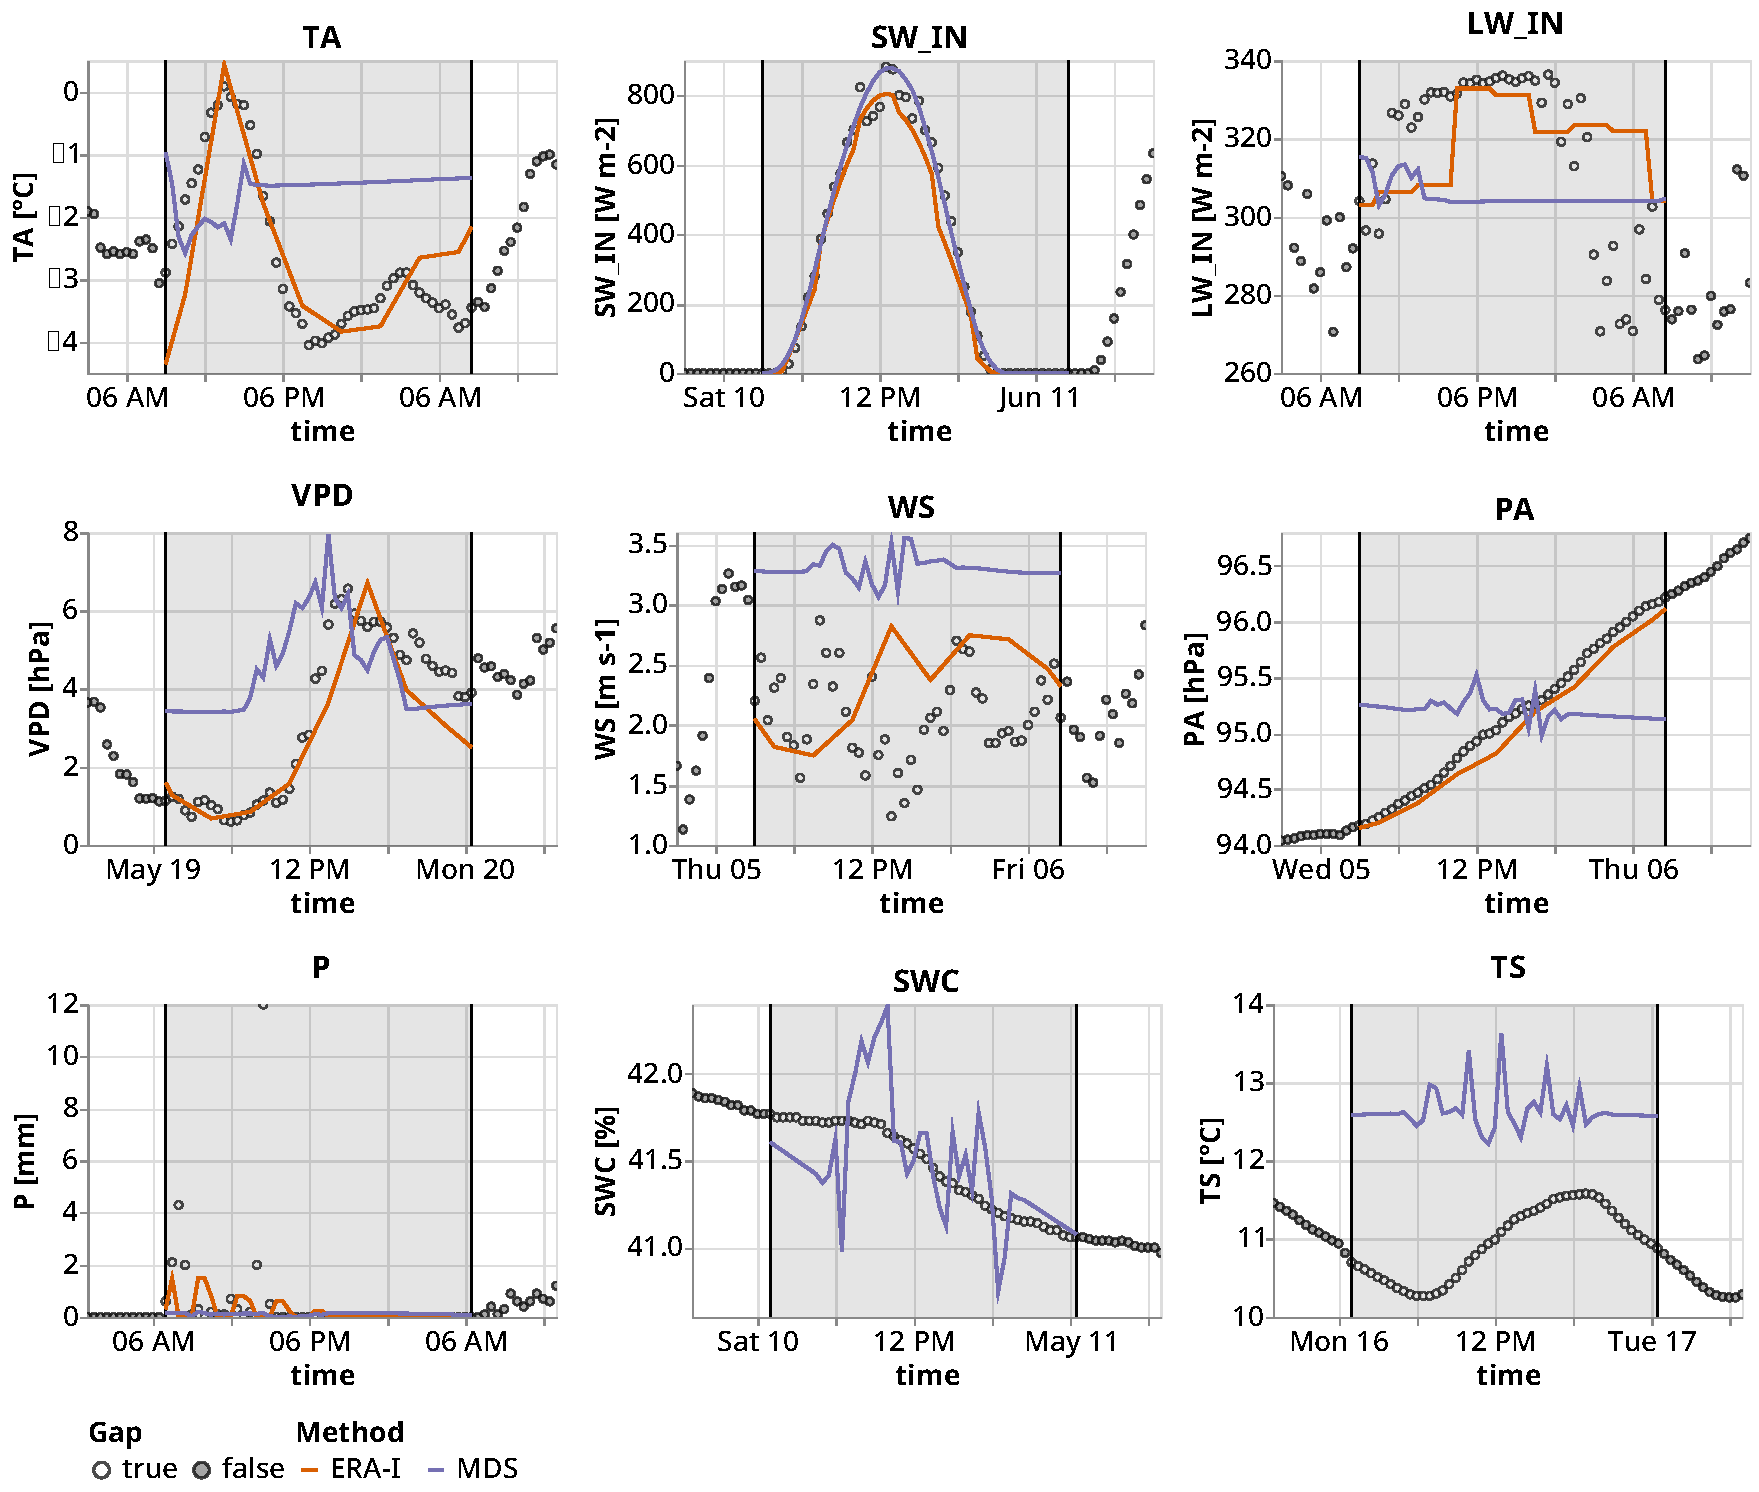
\includegraphics[width=\imgwidth]{timeseries_sota}}
\caption{Time series to visualize imputation using state-of-the-art methods: ERA-Interim (ERA-I in orange) and Marginal Distribution Sampling (MDS in purple). For each variable, one gap 24 hours long was created, with only one variable missing. The gray shaded area and the vertical black lines delimit the artificial gaps, where the observations are not available to the model but are used to assess the imputation performance.}
\label{fig:ts_sota}
\end{figure}

The imputation quality of the current methods is sometimes limited (Figure \ref{fig:ts_sota}). In particular, the imputation using MDS often results in relatively high error and unrealistic patterns. There are two possible directions to improve the accuracy of the imputation:  make a better use of the variables temporal autocorrelation; combine the information from ERA-I data and analysis of the local time serie for every prediction, instead of using the two approaches independently. Moreover, the current methods do not provide a measure of the uncertainty of the predictions.

\paragraph{Temporal autocorrelation} MDS uses the temporal autocorrelation only in a limited way, as it takes the average of the missing variable across the whole time window and does not weight the data depending on the proximity to the gap.  Similarly, the bias correction in ERA-I uses the entire dataset from a site, thus more importance is not assigned to the conditions around the gap.  This is a suboptimal use of available data, as the observations close to the gap have the highest correlation with the data in the gap and the meteorological variables have an overall high temporal autocorrelation (Figure \ref{fig:temp_autocorr}). This is particularly relevant for short and medium gaps (shorter than 1 week), which are the majority in the EC context.
In FLUXNET 2015 \cite{pastorello_fluxnet2015_2020}, the most extensive EC dataset with over 200 sites, almost 99 \% of gaps of meteorological variables are shorter than a week (appendix Figure \ref{fig:gap_len_dist}).

\paragraph{Combination of imputation approaches} \textsf{ONEFlux} employs both ERA-I and MDS, but the two methods are used independently, not combined for each prediction. The criteria to select the method to use is only the MDS quality control flags. The information on the missing data from temporal autocorrelation, dependency with other variables and other source of measurements (e.g. ERA-I) can be combined to make a more accurate prediction.

\paragraph{Uncertainty} A limitation of the current methods is the lack of a robust assessment of the uncertainty of the imputed values. MDS has a quality flag, but it is limited to only three possible values and it derives from constant thresholds. Moreover, in the final \textsf{ONEFlux} product, the quality flag indicates only which gap filling method was used. Ideally, each predicted data point has an associated uncertainty, which varies continuously and is interpretable, with the same physical unit of the variable.  In this way, the level of confidence of the model in each prediction is available to the data user. The uncertainty can be either used to discard the data when it is above a custom threshold, which can change depending on the application, or directly included in the downstream calculations.

\subsection{Contribution of this work}
In this work, I focused on a method that combines all three imputation approaches and includes interpretable quantification of uncertainty. Probabilistic machine learning algorithms are particularly suited, as they directly provide uncertainty for the predictions.
Gaussian Processes (GP) are one of the most important probabilistic algorithms \cite{2020_hennig_pml}. GP can model interactions between all data points, for example they can consider both a yearly and a daily pattern in the data. This, however, is connected to their main drawback: the computation cost scales cubically with the number of observations, making the use of GP computationally prohibitive. To overcome this limitation, several approximations, such as sparse GP, have been developed.
The Kalman Filter (KF) can be viewed as a special kind of GP, which models the time at discrete steps and where all the information about past and future observations is stored in a latent state. This drastically improves the computation efficiency, which scales linearly in the number of observations, but limits the ability to model processes with long time scales. However, in the context of EC meteorological imputation, this is an acceptable tradeoff as the majority of gaps are not long. Another advantage of the KF is the ability to include the ERA-I data in the predictions.

The aim of this work is to develop and test an imputation method for meteorological time series in the context of EC that employs a KF, as it promises more accurate predictions through a more efficient use of temporal autocorrelation in combination with the ERA-I data. Moreover, the KF provides a quantification of the predictions' uncertainty.
The imputation performance of the KF is evaluated by comparing it with the state-of-the-art methods (i.e. ERA-I and MDS). Then the aspects that affect the performance of the KF are assessed: the impact of the length of the gap, the advantage of including ERA-I data, the importance of inter-variable correlation and different training scenarios. The data from the EC site of Hainich, Germany, is used to train and evaluate the model.


\section{Methods}

\subsection{Kalman Filter theory}

Kalman Filter (KF) models over time a latent variable $x$, that represents the state of the system. The state cannot be directly observed, but it is possible to observe meteorological variables $y$ that reflect the state of the system.
KF is a probabilistic machine learning algorithm, so it keeps track of the entire distribution of the latent variable \cite{bishop_pattern_2006}.
The KF can update the state also when there are missing observations, hence the state is available for all time steps, which can in turn be used to predict the missing data points.

In order to model the state over time, assumptions on the behavior of the system are made. The first element is to model the time as a discrete variable.  Then there are three key assumptions: 1) the states are connected by a Markov chain, which means that the state at time $t$ depends only on the state at time $t-1$ and not on the states at previous times: $p(x_t|x_{t-1}) = p(x_t|x_{t-1}, x_{t-2}, \hdots, x_0)$; 2) the value of the observed variables depends on the latent state; 3) all the relationships are linear and all distributions are Gaussian. Additionally, the mean of the state at time $t$ may also depend on an external control variable $c_t$. This control variable does not depend on the state of the models, but provides information on the change of the state mean.
Equations \ref{eq:system_state} and \ref{eq:system_obs} describe the assumptions on the behavior of the system:

\begin{align}
p(x_t | x_{t-1}) &= \norm{x_t}{Ax_{t-1} + d + Bc_t}{Q} \label{eq:system_state}\\
p(y_t | x_t) &= \norm{y_t}{Hx_t + b}{R} \label{eq:system_obs}
\end{align}

The probability distributions of the state are computed using Bayesian inference. The computational cost of probabilistic inference is drastically reduced in this context, as can be performed using only linear algebra operations since all the relations are linear and all distributions are Gaussian.

The aim of the KF is to compute for every data point the probability distribution of the missing observations, $y^g_t$, given all the other observations, $Y^{ng}$, and the control variable, $C$: $p(\hat{y}^g_t \mid Y^{ng}, C$). To achieve this, the KF recursively computes intermediate distributions (Figure \ref{fig:kalman_filter}) with the same set of operations repeated for every time $t$.

The first step is to compute the \textit{predicted state}, $x^-_t$, that is obtained from the previous state, $x_{t-1}$, and the \textit{control variable}, $c_t$. This represents the conditional distribution of the state, given all observations until time $t-1$, $Y^{ng}_{0:t-1}$, and the control variable until time $t$: $C_{0:t}$, $p(x_t \mid Y^{ng}_{0:t-1}, C_{0:t})$.
The second step is to update the predicted state using the \textit{observations} at time $t$, $y_t$, to obtain the \textit{filtered state}, $x^f_t$. Observations can be partially or totally missing. This is the conditional distribution of the state given all the observation until time $t$: $p(x_t \mid Y^{ng}_{0:t}, C_{0:t})$.
These two steps make the filtering pass of the KF and are iteratively repeated for every time step in the observed dataset, starting from time $0$.
The last operation is to compute the smoothed state $x^s_t$, which is obtained by updating the filtered state using the information from the observations after time $t$. This computes the conditional distribution of the state given all the observations and control variables: $p(x_t \mid Y^{ng}, C)$.
Finally, the distribution of the missing observations, $p(y^g_t \mid Y^{ng}, C)$, can be computed directly from the smoothed state for each time step.

The model always considers the entire probability distribution for the state, which is a Gaussian distribution,  $p(x_t) = \norm{x_t}{m_t}{P_t}$, so stores for each state at each time step the mean, $m_t$, and the covariance, $P_t$. Similarly, the model predictions are a multivariate Gaussian distribution $p(y_t \mid Y^{ng}, C) =  \norm{y_t}{\mu_{y_t}}{\Sigma_{y_t}}$.

\begin{figure}
\centerline{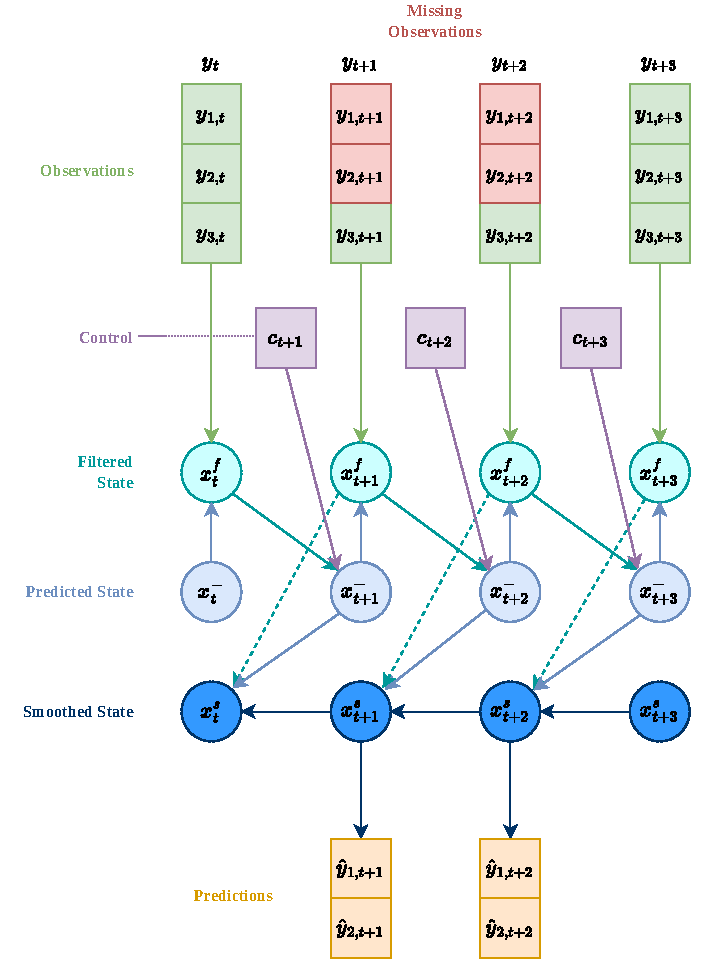
\includegraphics[width=4.5in]{Kalman Filter figure}}
\caption{Schematic representation of an example Kalman Filter. The green squares represent the observations of a single variable at a specific time, the observations may be missing (red squares). The blue circles represent the latent state, specifically the three versions of the state modelled by the KF: filtered state (cyan), predicted state (light blue) and smoother state (dark blue). The control variables are shown in purple.
All the arrows show a direct dependency for the computation of each element.}
\label{fig:kalman_filter}
\end{figure}

\paragraph{Time update}

The first step in a KF is computing the probability distribution of the predicted state $x^-_t$, from the filtered state at the previous time step $x^f_{t-1}$ and the control variable $c_t$.
The value of the control variable at time $t$ affects the value of state mean, but does not influence the state covariance.
The initial state of the system has the following distribution: $p(x_0) = \norm{x_0}{m_0}{P_0}$. Using Equation \ref{eq:system_state} and the properties of a linear map of Gaussian distributions the following equation can be derived \cite{bishop_pattern_2006, 2020_hennig_pml}:

\begin{equation}
\begin{aligned}\label{eq:time_update}
    p(x_t \mid Y^{ng}_{0:t-1}, C_{0:t}) &= \norm{x_t}{m_t^-}{ P_t^-}\\
    m_t^- &= Am_{t-1} + B c_t + d \\
    P_t^- &= AP_{t-1}A^\top + Q
\end{aligned}
\end{equation}

\paragraph{Measurement update}

The predicted state is updated to obtain the distribution of the filtered state, using the current observation $y_t$. Equation \ref{eq:system_obs} describes the distribution of $y_t$ given $x_t$. Using Bayes' theorem, it is possible to compute the distribution of $x_t$ given an observation, $y_t$ \cite{bishop_pattern_2006, 2020_hennig_pml}:

\begin{equation}
\begin{aligned}
     p(x_t \mid Y^{ng}_{0:t}, C_{0:t}) &= \mathcal{N}(x_t; m_t, P_t) \label{eq:meas_update}\\
     z_t &= Hm_t^- + d \\
     S_t &= HP_t^-H^\top + R \\
     K_t &= P_t^-H^\top S_t^{-1} \\
     m_t &= m_t^- + K_t(y_t - z_t) \\
     P_t &= (I-K_tH)P_t^-
\end{aligned}
\end{equation}

\subparagraph{Missing observations}

The KF is able do deal with missing observations and can update the state even in that case.
If all the observations at time $t$ are missing, the measurement update step is skipped and the filtered, $x^f_t$, is the same of the predicted state, $x_t^-$. If only some observations in $y_t$ are missing, then a partial measurement step is performed.
The vector containing the observations that are not missing at time $t$, $y^{ng}_t$, can be expressed as a linear transformation of $y_t$:
\begin{equation}\label{eq:miss_obs}
    y^{ng}_t = M^{ng}_ty_t
\end{equation}
where $M^{ng}_t$ is a mask matrix that is used to select the subset of $y_t$ that is observed. $M_t^{ng} \in \mathbb{R}^{n^{ng} \times n}$, $y_t \in \mathbb{R}^n$, and $y_t^{ng} \in \mathbb{R}^{n_{ng}}$. The mask is made of rows which are all zeros, but for an entry 1 at the column corresponding to the of the index of the non-missing observation.

For example, if $y_t = [y_{0,t}, y_{1,t}, y_{2,t}]^\top$ and $y_{0,t}$ is the missing observation, then:
\begin{equation*}
 M^{ng}_t = \left[\begin{array}{ccc}
    0 & 1 & 0 \\
    0 & 0 & 1
\end{array}\right]
\end{equation*}

Using the properties of linear projections of a Gaussian distribution, it is possible to derive the distribution $p(y^{ng}_t \mid x_t)$ from $p(y_t \mid x_t)$:
 \begin{align*}
   p(y^{ng}_t|x_t) = p(M^{ng}_ty_t|x_t) &=   \norm{y^{ng}_t}{M^{ng}_tHx_t + M^{ng}_tb}{M^{ng}_tR(M^{ng}_t)^\top}%\label{eq:partial_obs_state}
\end{align*}
Therefore, it is possible to perform the measurement update step when some observations are missing using a variation of Equation \ref{eq:meas_update}, where $H$ is replaced by $M^{ng}H$, $b$ by $M^{ng}b$ and $R$ by $M^{ng}R(M^{ng})^\top$. In this way, $H$ varies between each time step depending on which variables are missing.

\paragraph{Smoothing}

In the smoothing step, the filtered state at time $t$ is updated using the observations after time $t$. A widely applied set of equations for the smoothing pass is the Rauch-Tung-Striebel Smoother \cite{rauch_maximum_1965}. They calculate the smoothed state, $x_t^s$, from the filtered state and time $t$, and the smoothed and filtered and at time $t+1$:
\begin{equation}
\begin{aligned}\label{eq:smoother}
    p(x_t \mid Y^{ng}, C) &= \norm{x_t}{m_t^s}{P_t^s} \\
    G_t &= P_tA^\top(P_{t+1}^-)^{-1}\\
    m_t^s &= m_t + G_t(m_{t+1}^s - m_{t+1}^-) \\
    P_t^s &= P_t + G_t(P_{t+1}^s - P_{t+1}^-)G_t^\top
\end{aligned}
\end{equation}
For the last time step, the smoothed state is set to be equal to the filtered state.

\paragraph{Predictions} The predicted distribution of the observed variables in a gap, $\hat{y}^g_t$, can be obtained directly by the distribution of the smoothed state, $p(x_t | Y^{ng}, C)$.
The missing observed variables a time $t$ are $y^g_t = M^g_ty_t$, where $M^{g}$ has a similar definition as $M^{ng}_t$ in Equation \ref{eq:miss_obs}, but selects the missing observations instead of non-missing data.
The following equation can see derived (appendix Equation \ref{eq:deriv_predictions}):

\begin{equation}
\begin{aligned}\label{eq:filter_predictions}
    p(\hat{y}^g_t \mid Y^{ng}, C) &= \norm{\hat{y}^g_t}{\mu_{y_t}}{\Sigma_{y_t}} \\
    \mu_{y_t} &= M^g_tHm_t + M^g_tb \\
    \Sigma_{y_t} &= M^g_tR(M^g_t)^\top + M^g_tHP^s_tH^\top (M^g_t)^\top
\end{aligned}
\end{equation}

The output of the KF model is the distributions of $p(y^g_t)$ for all gaps in the observed variables.

\subsection{Kalman Filter implementation}

% \paragraph{Requirements}

KF is a widely used algorithm and there are several python libraries that implement it (e.g. \textsf{statsmodels}, \textsf{pykalman}, \textsf{filterpy}). However, no  KF library was identified which meets all the requirements for this work. It is necessary to support gaps, partial measurements updates, control variables and be a numerically stable implementation.
Therefore, a custom library for KF was developed using the \textsf{PyTorch} library, which has the advantage of automatic differentiation, possibility to use GPUs and better integration with other Machine Learning methods.

\subsubsection{Numerical stability}

% \paragraph{Background}
The naive implementation of the KF equations suffers from numerically stability issues \cite{mohinder_s_grewal_kalman_2001, dan_simon_optimal_2006}. %, hence several techniques have been developed to mitigat
Numerical instability arises from the fact that digital computers store numbers with only limited precision, which also varies depending on the value of the number. This results in a loss of information, so that some operations may be incorrectly performed by a  computer (e.g. summing a big number and a small number).

For KF the components that are most affect by numerical instability are the covariance matrices. To analyze the stability of the operations on these matrices it is relevant to consider the condition number for inversion \cite{mohinder_s_grewal_kalman_2001, kaminski_discrete_1971}, which provides an indication if the matrix is going to be singular on the numerical representation in the computer. The condition number $k(A)$ is the ratio between the biggest singular value and the smallest. The singular value is $\sigma^2(A) = \lambda(AA^\top)$, with  $\lambda(A)$ being the eigenvalue of $A$:
\begin{equation*}%\label{condition_number}
    k(A) = \frac{\sigma_{max}(A)}{\sigma_{min}(A)}
\end{equation*}
The condition number is 1 for well-conditioned matrices, and tends to infinite for ill-conditioned matrices. As a general rule,  a matrix cannot be inverted when the reciprocal of the condition number for inversion is close to the machine precision $ 1/k(A) < \varepsilon$ \cite{mohinder_s_grewal_kalman_2001}.

\paragraph{Mitigation strategies}
% \subparagraph{Machine precision}
The simplest approach to improve the numerical stability is to use higher accuracy in the representation of numbers \cite{dan_simon_optimal_2006}. Practically, this means to use 64 bit floats instead of 32 bit floats, which is the default in \textsf{PyTorch}.

% \subparagraph{Matrix decomposition}
Another way to improve the numerical stability is to reduce the condition number of the state covariance, $P$. A positive definite matrix has a square root factor, $P^{1/2}$, such as that $P = P^{1/2}(P^{1/2})^\top=P^{1/2}P^{\top/2}$.
The Cholesky decomposition is an algorithm to find a square root of a matrix, however the Cholesky decomposition calculates only one of possibly many square roots of the matrix.

Utilizing $P^{1/2}$ instead of $P$ doubles the effective numerical resolution of the KF \cite{kaminski_discrete_1971,dan_simon_optimal_2006,rutten_square-root_2013}. This is due to the fact that the eigenvalues of $P^{1/2}$ are the square root of the eigenvalues of $P$, $\lambda(P) = \lambda^2(P^{1/2})$, thus the conditioning number of $P$ is the square of the conditioning number of $P^{1/2}$. Therefore, if in the KF implementation $P$ is never explicitly computed, the numerical stability of the KF is significantly improved.
There are several implementations of a KF that follow this approach \cite{potter_statistical_1963,carlson_fast_1973,bierman_numerical_1977} and are generally called ``square root'' filter.

\paragraph{Implementation in PyTorch}
There are different approaches to square root filtering. According to \textcite{mohinder_s_grewal_kalman_2001} the best approach is the UD-Filter \cite{bierman_numerical_1977}, since it has the smallest computational cost. However, the filter is based on the $UD$ factorization and a custom matrix factorization \cite{mohinder_s_grewal_kalman_2001} and both of those algorithms cannot be efficiently implemented in \textsf{PyTorch}. The \textsf{PyTorch} function \verb|torch.linalg.ldl_factor| performs a $UD$ factorization, but it is an experimental function and is not differentiable. Moreover, the custom matrix factorization would need to be implemented using scalar operations, which are not efficient with \textsf{PyTorch} eager execution.

For this reason, a square root filter that propagates square roots of the covariance matrices is implemented. In this way, all the required computations can be expressed in QR factorization, which is a numerically stable routine and is implemented in \textsf{PyTorch}.

\paragraph{Time update Square Root Filter}

From the equations of the time update step (Equation \ref{eq:time_update}), it is possible to derive an algorithm to obtain $P_t^{1/2}$ given $P_{t-1}^{1/2}$ \cite[eq. 6.60]{mohinder_s_grewal_kalman_2001}. Defining:
\begin{equation*}
    W = \begin{bmatrix}AP_{t-1}^{1/2} & Q^{1/2}\end{bmatrix}
\end{equation*}
from Equation \ref{eq:time_update} the following is true:
% \begin{equation*}\label{time_update_SR_mult}


\begin{align*}
    % WW^\top &= P_t \\
  WW^\top &=  \begin{bmatrix}AP_{t-1}^{1/2} & Q^{1/2}\end{bmatrix}\begin{bmatrix}P_{t-1}^{\top/2}A^\top \\ Q^{\top/2}\end{bmatrix}
  \\ &= AP_{t-1}^{1/2}P_{t-1}^{\top/2}A^\top + Q^{1/2}Q^{\top/2} = AP_{t-1}A^\top + Q\\ &= P_t
\end{align*}

The next step is to factorize  $W=LU$, where $L$ is a lower triangular matrix and $U$ is an orthogonal matrix, such as that $UU^\top = I$. Then $WW^\top = LU(LU)^\top = LUU^\top L^\top = LL^\top=P_t$. Hence, $L$ is a square root of $P_t$.
This procedure never explicitly computes $P_t$ and requires only the factorization of a matrix, which is implemented efficiently and in a numerical stable way in the \textsf{PyTorch} \verb|torch.linalg.qr| function.
PyTorch does not support natively a $LU$ decomposition, but it implements the QR factorization: $W=QR$, where $Q$ is an orthogonal matrix and $R$ an upper triangular matrix. This can be used to compute the $LU$ factorization by performing a $QR$ factorization of $W^\top$ and defining $L = R^\top$, as $W=(W^\top)^\top=(QR)^\top=R^\top Q^\top=LU$.
The steps of the Square Root time update are:

\begin{enumerate}
    \item let  $W = \begin{bmatrix}AP_{t-1}^{1/2} & Q^{1/2}\end{bmatrix}$
    \item do the $LU$ factorization $W=LU$
    \item set $P_t^{1/2} = L$
\end{enumerate}

\paragraph{Measurement update Square Root Filter} A similar procedure can be followed for the measurement update step of the filter \cite{dan_simon_optimal_2006}. The starting point is Equation \ref{eq:meas_update}, for simplicity the time subscripts are omitted in the following equations. Defining:
\begin{alignat*}{3}
    M &= \begin{bmatrix} R^{1/2} & H(P^-)^{1/2} \\ 0 & (P^-)^{1/2} \end{bmatrix} \quad &
    V &= \begin{bmatrix} S^{1/2} & 0 \\ \bar{K} & P^{1/2} \end{bmatrix} \quad&
    \bar{K} &= KS^{1/2}
\end{alignat*}

then $MM^\top = VV^\top$ (appendix Equation \ref{eq:deriv_meas_update_sr}). Therefore, by decomposing $M=LU$, then $MM^\top=LL^\top=VV^\top$ and the bottom right block of size $k \times k$ of $L$ is a square root of $P$, where $k$ is the number of dimensions of the state, $x_t \in \mathbb{R}^k$.
The steps of the Square Root measurement update are:
\begin{enumerate}
 \item let $M = \begin{bmatrix} R^{1/2} & H(P^-)^{1/2} \\ 0 & (P^-)^{1/2} \end{bmatrix}$
 \item do the $LU$ factorization of $M=LU$
 \item $P^{1/2}$ is the bottom right $k \times k$ block of $L$
\end{enumerate}

\paragraph{Predictions Square Root Filter} The prediction equations for the square root filter are similar to the equations for the time update. Defining:
\begin{equation*}
    W = \begin{bmatrix}HP_{t}^{1/2} & R^{1/2}\end{bmatrix}
\end{equation*}

from Equation \ref{eq:filter_predictions} the following is true:
\begin{align*}
  WW^\top &=
  \begin{bmatrix}HP_{t}^{1/2} & R^{1/2}\end{bmatrix}\begin{bmatrix}P_{t}^{T/2}H^\top & R^{\top/2}\end{bmatrix} \\
  &= HP_{t}^{1/2}P_{t}^{\top/2}H^\top + R^{1/2}R^{\top/2} = HP_{t}H^\top + R \\ &= \Sigma_{y_t}
\end{align*}

The steps of the Square Root predictions are:
\begin{enumerate}
    \item let  $W = \begin{bmatrix}HP_t^{1/2} & R^{1/2}\end{bmatrix}$
    \item do the LU factorization of $W=LU$
    \item set $\Sigma_{y_t}^{1/2} = L^\top$
\end{enumerate}

\paragraph{Smoothing Square Root Filter} The available literature for implementing a square root smoother is scarce compared to a square root filter. Therefore no solution has been identified to implement a square root smoother and a standard smoother is employed.
Nonetheless, steps were taken to improve the numerical stability of the smoother.
The computation in the smoother that is most numerically unstable is the inversion of $P^-_{t+1}$ in Equation \ref{eq:smoother} \cite{mohinder_s_grewal_kalman_2001}. The matrix inversion is avoided by using the \verb|torch.cholesky_solve| function. It solves for $X$ the linear system $P^-_{t+1}X=P_tA$, which is equivalent of computing $X = (P_tA^\top(P^-_{t+1})^{-1})^\top$. This uses directly the square root $(P^-_{t+1})^{1/2}$ to avoid the computation of $P^-_{t+1}$. A further step to improve the numerical stability is forcing the covariance matrix to be symmetric, by averaging to upper and lower part at after every time step, $P^s_{t, sym} = (P^s_t + (P^s_t)^\top)/2$, as suggested in \textcite{dan_simon_optimal_2006}.
This approach to numerical stability in the smoother is the same as applied by the \textsf{statsmodels} library \cite{noauthor_statsmodelstsastatespacekalman_filterkalmanfilter_nodate}.

\subsection{Kalman Filter model}

\paragraph{Parameters}

\begin{table}[H]
\caption{Parameters of the Kalman Filter Model. $n$ is the number of dimension of the observations, $k = 2n$ the number of dimensions of the state, $n_{ctr}$ the number of dimensions of the control variable.}
\label{table:parameters}
\vspace{5pt}
\centering
\begin{tabular}{l c c c}
\toprule
    \bfseries Parameter name & \bfseries Notation & \bfseries Shape & \bfseries Initial value\\
    \hline
    \noalign{\vspace{4pt}}
    State transition matrix & $A$ & $k \times k$ & $\begin{bmatrix}I & I \\ 0 & I\end{bmatrix}$ \\
    \noalign{\vspace{4pt}}
    Observation matrix & $H$ & $n \times k$ & $\begin{bmatrix}I & 0 \end{bmatrix}$ \\
    \noalign{\vspace{4pt}}
    State transition covariance & $Q$ & $k \times k$ & $\text{diag}(0.1)$ \\
    \noalign{\vspace{4pt}}
    Observation covariance & $R$ & $n \times n$ & $\text{diag}(0.01)$\\
    \noalign{\vspace{4pt}}
    State transition offset & $d$ & $k$ & 0 \\
    \noalign{\vspace{4pt}}
    Observation offset & $b$ & $n$ & 0 \\
    \noalign{\vspace{4pt}}
    Control matrix & $B$ & $k \times n_{ctr}$ & $\begin{bmatrix} -I & I \\ 0 & 0 \end{bmatrix}$ \\
    \noalign{\vspace{4pt}}
    Initial state mean & $m_0$ & $k$ & $0$ \\
    \noalign{\vspace{4pt}}
    Initial state covariance & $P_0$ & $k \times k$ & $\text{diag}(3)$ \\
\bottomrule
\end{tabular}
\end{table}

The KF is implemented as \textsf{PyTorch} module, whose parameters are described in Table \ref{table:parameters}.
There is no change over time of the parameters, and the state of the KF is initialized always at the same value from the parameters $m_0$ and $P_0$.

% \paragraph{Constraint}

An important aspect for implementing a KF in \textsf{PyTorch} is constraining the parameters that represent covariance ($Q$, $R$ and $P_0$) to be positive definite \cite{bishop_pattern_2006}. To achieve this goal, the optimizer works on a raw parameter, which is then transformed into a positive definite matrix.
The transformation into a positive definite matrix is done by transforming the raw parameter into a lower triangular matrix with a positive diagonal. The diagonal is enforced to be positive by transforming the diagonal of the raw parameter with the softplus function, $x = \log (1 + e^{x})$, which is a positive function. In addition, a small positive offset, $\num{1e-5}$, is added to the diagonal in order to avoid that the diagonal is close to zero, which may result in a positive semi-definite matrix. This implementation of the positive definite constraint makes it straightforward to obtain the Cholesky factor of the parameters, which are needed by the Square Root Filter, and at the same time the full parameters, which are needed by the smoother.

\subparagraph{Parameters initialization}

The model parameters could be initialized using random values, however this would increase numerical stability issues and increase the training time. Moreover, if the initial parameters are very distant from the optimal ones, it is more likely for the optimization algorithm to find only a local minimum.  The simplicity of the KF and the interpretability of its parameters allows to manually initialize the parameters with realistic values.

The parameters are initialized using a local linear trend model \cite{durbin_time_2012-1}. It assumes that the state of the system, $x_t$, is made by two components, the level $x_{l_t}$ and the slope, $x_{s_t}$: $x_t = [x_{l_t}, x_{s_t}]^\top$ . The observed variable, $y_t$, is equal to the state level with an addition of Gaussian white noise, $\varepsilon_t$; the state level is the sum of the previous state levels, $x_{l_{t-1}}$. The previous state slope, $x_{l_{t-1}}$, and a Gaussian white noise component, $\nu_{t-1}$. The state slope is equal to the previous slope, $x_{s_{t-1}}$, and another Gaussian white noise component, $\xi_{t-1}$:
\begin{equation*}
   \begin{alignedat}{2}
    y_t &= x_{l_t} + \varepsilon_t & p(\varepsilon_t) \quad &= \norm{\varepsilon}{0}{R}\\
    x_{l_t} &= x_{l_{t-1}} + x_{s_{t-1}} + \nu_{t-1} \quad \quad & p(\nu_{t-1}) &= \norm{\nu}{0}{Q_\nu}\\
    x_{s_t} &= x_{s_{t-1}} + \xi_{t-1} \quad & p(\xi_{t-1}) &= \norm{\xi}{0}{Q_\xi} \\
    % x_t &= \begin{bmatrix} x_{l_t} \\ x_{s_t} \end{bmatrix} &&
    \end{alignedat}
\end{equation*}

A KF can be used to model a system described above by selecting suitable parameters:

\begin{equation*}\label{eq:local_slope}
\begin{alignedat}{3}
    A &= \begin{bmatrix}I & I \\ 0 & I\end{bmatrix} \quad & Q &= \begin{bmatrix}Q_\varepsilon & 0 \\ 0 & Q_\nu \end{bmatrix}  \quad & H &= \begin{bmatrix}I & 0 \end{bmatrix}
\end{alignedat}
\end{equation*}

The use of the slope component allows the KF to retain information about several previous and following observations, while a KF with only a level compotent would be limited to use only the obsevation one time step before or after the gap.

The local slope model can be extended by adding the state and observations offsets $d$ and $b$ and a control variable similarly to Equations \ref{eq:system_obs} and \ref{eq:system_state}.
In the context of this work, the ERA-I dataset is used for the control variable. The control variable should quantify the change between consecutive states levels, so the difference between consecutive ERA-I observations is used. This can be achieved by setting the control variables to $c_t = [\text{ERA-I}_t, \text{ERA-I}_{t-1}]^\top$ and uses the control matrix to compute the difference between the ERA-I observations. Moreover, the control variable should have no effect on the state slope. An issue with this approach arises from the fact that some variables are not present in the ERA-I (i.e. $n_{ctr} < n$), thus there is not a one to one correspondence between the control variable and the observed variable, and hence the state level. This is solved by sorting the variables in a way that there is correspondence between the first $n_{ctr}$ observed variables and the ERA-I variables. For those reason, the control matrix is initialized in such a way that the control variable influences only the level of the first $n_{ctr}$ dimensions of the state level:
\[
B = \begin{bmatrix}-I & I \\ 0 & 0\end{bmatrix} \quad B \in \mathbb{R}^{k \times n_{ctr}} \quad I \in \mathbb{R}^{n_{ctr} \times n_{ctr}}
\]
The state transition covariance $Q$ and then observation covariance $R$ are initialized as diagonal matrix with values of $0.1$ and $0.01$ respectively. These numbers have been chosen to represent an uncertainty in the state transition that is compatible with the standard deviation of the variables (i.e $\sigma = 1$ after standarization) and a low uncertainty in the observations.

The observation and state transition offsets are initialized to zero. The initial state is set to have as mean zero and as covariance $\text{diag}(3)$. The number 3 is an arbitrary number bigger than the state transition covariance, which represents an high level of uncertainty for the initial state.

\paragraph{Loss Function}

The loss function used to train the model is the negative log likelihood, computed for each data point. At each time step, the model predicts a multivariate normal distribution $p(\hat{y}^g_t \mid Y^{ng}, C)$, which is used to compute the negative log likelihood given the actual observations $y_t^g$. The negative log likelihoods between different time steps in the same gap are summed, while the negative log likelihood is averaged between batches.
The actual loss function of the model should be the log likelihood of the joint distribution $p(Y^g|Y^{ng}, C)$. However, the analytical form of the joint distribution cannot be easily derived from the KF equations. The log likelihood of marginal distributions is instead used, as it is a lower bound to the log likelihood of the joint distribution. Defining: $q(x)$ the predicted joint distribution, $p(x)$ the real joint distribution and $q_i(x)$ the marginal distribution at the \textit{i}th time step:
\begin{equation*}
    q_i(x) = \int q(x_1, ..., x_k)dx_{\neg i}
\end{equation*}

If the family of distribution of $q(x \mid \theta)$,  is the same of $\prod_i q_i(x \mid \theta)$, where $\theta$ are the model parameters; then:

\begin{equation}\label{eq:log_joint_geq}
    \max_\theta \E{\log q(x\mid \theta)}_{x \sim p(x)} \geq \max_\theta \E{\log \prod_i q_i(x\mid \theta)}_{x \sim p(x)}
\end{equation}

because $\prod_i q_i(x)$ is more restricted. This means that $q(x)$ fits at least as good as $\prod_i q_i(x)$.
For the KF $q_i(x)$ is a Gaussian distribution, so $\prod_i q_i(x)$ is also a Gaussian distribution and Equation \ref{eq:log_joint_geq} holds.

\paragraph{Metrics} The main metric used to assess the model performance is the \emph{Root Mean Square Error} (RMSE):
\begin{equation*}
    \text{RMSE} = \sqrt{\frac{\sum_i^n (y^g_i - \hat{y}^g_i)^2}{n}}
\end{equation*}

The advantage of the RMSE is that it can also be used for non-probabilistic methods (e.g. MDS) and that its value has the same physical dimension as the observed variable. The main drawback is that it cannot be used for comparison between variables. For that, the \emph{Standardized} RMSE is used, which is the RMSE computed on the standardized variables (Equation \ref{eq:standardized}). It can be computed by transforming the RMSE (appendix Equation \ref{eq:deriv_stand_rmse}):
\begin{equation*}
    \text{RMSE}_{\text{stand}} = \frac{\text{RMSE}}{\sigma_Y}
\end{equation*}

Other metrics, like the $R^2$ score and the Mean Absolute Percentage Error (MAPE) were evaluated, however none of them are suitable for this application. The $R^2$ is defined as $R^2 = 1 - (\sum_{i}^{n} (y_i - \hat{y}_i)^2)/(\sum_{i}^{n} (y_i - \bar{y})^2)$, if the denominator is close to zero, then value of $R^2$ tends to $- \infty$. Since the gaps are often short and several variables are constant over short periods (e.g. \vv{SW\_IN}, \vv{SWC}) the denominator of the $R^2$ would be close to zero and the metrics cannot be effectively used. The mean absolute percentage error is defined as $\text{MAPE} = \frac{1}{n} \sum_{i=0}^{n_-1} (\left| y_i - \hat{y}_i \right|)/(\left| y_i \right|)$, which tends to $\infty$ when $y_i$ tends to 0, as zero is a possible value of several variables (e.g. \vv{SW\_IN}, \vv{TA}) this metric cannot be employed.
It would be possible to use $R^2$ or MAPE for a subset of variables and gap lengths, but this limits the ability to perform comparisons across different settings.

\paragraph{Performance considerations}

The iterative nature of the KF, where the current state depends on the previous state, makes it impossible to use \textsf{PyTorch} vectorization across different time steps. This can significantly limit the performance of the KF, especially when executed on GPUs. In order to  mitigate this issue, all functions in the KF library support batches, so at every time step different data is processed in parallel.


\subsection{Data}

\paragraph{Data source} The data used to evaluate the performance of the KF is from the Hainich (Germany) site. The EC site in Hainich (DE-Hai) is on a deciduous beech forest and it is managed by the bioclimatology department at the  University of Göttingen. The source of the data is  the FLUXNET 2015 Dataset \cite{pastorello_fluxnet2015_2020}, which for Hainich includes measurements with a 30 minutes frequency between 2000 and 2012. In total 227952 observations are available. For simplicity, the entire dataset was used for the model training, which includes also gap-filled observations.
All the meteorological variables that are gap-filled in the FLUXNET 2015 dataset were selected for the analysis (Table \ref{table:variables}).

The FLUXNET 2015 dataset also includes the ERA-I dataset for each site. The data is bias corrected and temporally downscaled.
The ERA-I data is used as the control variable for the KF. All the variables of interest are present in ERA-I, except for \vv{TS} and \vv{SWC}.

\begin{table}[H]
\caption{Meteorological variables used to evaluate the Kalman Filter imputation. ERA-I column indicates whether the variable is available in the ERA-Interim dataset.}
\label{table:variables}
\vspace{5pt}
\centering
\begin{tabular}{l>{\bfseries}llc}
\toprule
    \bfseries Variable mame & \bfseries Abbreviation & \bfseries Unit & \bfseries ERA-I \\
    \hline
    Air Temperature & \lstinline|TA| & \si{^{\circ}C} & \ding{51}\\
    Incoming Shortwave Radiation & \lstinline|SW_IN| & \si{W/m^2} & \ding{51}\\
    Incoming Longwave Radiation & \lstinline|LW_IN| & \si{W/m^2} & \ding{51}\\
    Vapour Pressure Deficit & \lstinline|VPD| & \si{hPa} & \ding{51}\\
    Wind Speed & \lstinline|WS| & \si{m/s} & \ding{51}\\
    Air Pressure & \lstinline|PA| & \si{hPa} & \ding{51}\\
    Precipitation & \lstinline|P| & \si{mm} & \ding{51}\\
    Soil Temperature & \lstinline|TS| & \si{^{\circ}C} & \ding{56} \\
    Soil Water Content & \lstinline|SWC| & \si{\percent} & \ding{56}\\

\bottomrule
\end{tabular}
\end{table}


\paragraph{Data preparation pipeline}

The dataset needs to be pre-processed by dividing it into data blocks, adding an artificial gap and then standardize. The data preparation pipeline takes as input a list of items and outputs the data in a format suitable for training. Each item provides all the information about a gap with the following fields: a) \verb|i| the index of the block; b) \verb|shift|  the offset of the data block; c) \verb|var_sel| the variables missing in the gap; d) \verb|gap_len| the gap length. The pipeline performs the following steps: 1) splits the index of complete data frame from Hainich into blocks of a given length and selects the \texttt{i}\textsuperscript{th} element;  2) adds the shift to move the starting point of the data block and select the data from the data frame. For ERA-I it also adds the observations with a lag 1, so that at the time $t$ the model has access to the ERA-I observations both at time $t$ and $t-1$; 3) creates one continuous artificial gap in the middle of the block for the variables specified in \verb|var_sel| and with a length of \verb|gap_len| 4) converts from \textsf{Pandas} data frame to a \textsf{PyTorch} tensor 5) standardizes each variable, using the mean, $\mu_Y$, and standard deviation, $\sigma_Y$, of the whole dataset:
\begin{equation}\label{eq:standardized}
    y^z_t = \frac{y_t - \mu_Y}{\sigma_Y}
\end{equation}
After this, the tensors are collated into a batch and potentially moved to the GPU.

\paragraph{Prediction pipeline} The model predicts the mean and the covariance for each time steps for the standardized variables. This needs to be converted back to be scale of the variable to be used for imputation. This operation should scale the whole distributions and not only the mean of the prediction. The standardized prediction $\hat{y}^z_t$ is distributed $p(\hat{y}^z_t) = \norm{\hat{y_t}^z}{\mu^z_{\hat{y_t}}}{\Sigma^z_{\hat{y_t}}}$, the prediction in the original scale $\hat{y}_t$ is distributed $p(\hat{y}_t) =  \norm{\hat{y_t}}{\mu_{\hat{y_t}}}{\Sigma_{\hat{y_t}}}$. From the inverse of Equation \ref{eq:standardized}:

\begin{equation*}
    \hat{y}_t = \Sigma_Y\hat{y}^z_t + \mu_Y
\end{equation*}

where $\Sigma_Y = \text{diag}(\sigma_Y)$. Then, using the properties of the linear projections of Gaussian distributions:

\begin{equation*}
    p(\hat{y}_t) = \norm{\hat{y}_t}{\Sigma_Y\mu^z_{\hat{y_t}} + \mu_Y}{\Sigma_Y\Sigma^z_{\hat{y_t}}\Sigma_Y^\top}
\end{equation*}

\subsection{Model training}

The available data is split between training and validation set, the first 80\% of the data points are used for training, the remaining 20\% for validation. The split is not random, so the validation set does not contain periods of time close to the ones used for training.

The KF is initialized with 9 dimensions for the observations (one for each variable). For the state 18 dimensions, the first 9 dimensions are the state level while the other 9 are for the state slope of the local trend model. The control has 14 dimensions, with 7 for the control at time $t$ and the other 7 for the control at time $t-1$.

The model is trained using gradient descend, by minimizing the loss function. It employs the ADAM optimizer \cite{kingma_adam_2017}. The learning was manually stopped when the training loss started being constant or the validation loss started to increase.

Several versions of the KF are trained using data with different patterns in the gaps. Figure \ref{fig:training} shows the different combinations. Each model version is named in a way to reflect to training conditions and it uses this pattern: \textit{KF-\textlangle var missing\textrangle-\textlangle n var missing\textrangle-\textlangle range gap lengths\textrangle[-\textlangle modifier\textrangle]}.

\paragraph{Generic model} The first model to be trained is a generic model (\textbf{KF-Gen-Sin-6\_336}), where each data block had a gap in one variable with the length sampled from a uniform distribution between \num{6} (3 hours) and \num{336} (1 week). For each gap, only one variable was missing, which was sampled with equal probability from the list of all variables. The shift was sampled from a normal distribution with mean 0 and standard deviation 50. For each block of data in the original data frame, 10 different artificial gaps were created, resulting in a total of 4080 data blocks used for training and 520 for validation.
The length of the block of data was \num{446}, so that at least \num{50} observations were available to the model before and after the gap. The batch size was \num{20}.
The model was trained for \num{3} epochs with a learning rate of \num{1e-3}.

\paragraph{Variable fine-tuning} The generic model was fine tuned for each variable (\textbf{KF-\textlangle var\textrangle-Sin-6\_336}), resulting in 9 different models. The training settings were the same for the generic model, expect that the gaps were only in one variable and then number of repetitions for each was 5 (training 2040 blocks, validation 260 blocks). Each variable was fine-tuned with a different combination of epochs and learning rate (lr):
\begin{itemize}
    \item \vv{TA} 3 epochs with lr \num{1e-3} and 1 epoch with lr \num{1e-5}
    \item \vv{SW\_IN} \num{7} epochs with lr \num{1e-3}
    \item \vv{LW\_IN} \num{3} epochs with lr \num{1e-3}, \vv{VPD} \num{6} epochs with lr \num{1e-3}
    \item \vv{VPD} \num{5} epochs with lr \num{1e-3}
    \item \vv{WS} \num{3} epochs with lr \num{1e-3}
    \item \vv{PA} \num{3} epochs with lr \num{1e-3} and 1 epoch with lr \num{1e-5}
    \item \vv{P} no additional training
    \item  \vv{TS} \num{6} epochs with lr \num{1e-3}
    \item \vv{SWC} \num{8} epochs with lr \num{1e-3} and 1 epoch with lr \num{1e-5}
\end{itemize}

\paragraph{Short gaps} The numerical stability issue limits the gap length to 30 observations (15 hours) if all variables are missing. Therefore, an additional set of models was trained with for short gaps up to 15 hours, in order to have multiple variables missing.
A version of the model was trained only with gaps in all variables (\textbf{KF-Gen-All-6\_30}). The length of the gap ranged from 6 to 30 (3 to 15 hours). The training set contained 7000 unique data blocks and 1760 for validation. The training started from the generic model and lasted for 3 epochs, with a learning rate of \num{3e-4}.

The generic model was also fine-tuned for short gaps (\textbf{KF-Gen-Sin-6\_30}). The training was for 3 epochs with a learning rate of \num{3e-4}.

Another version of the model was trained with gaps in any number of variable (\textbf{KF-Gen-Multi-6\_30}). The number of variables missing was drawn from a uniform distribution  from 1 to $n$, and the variables missing sampled with equal probability. The total gap length ranged from 6 to 30 (3 to 15 hours). For each original data block, 20 different artificial gaps were generated for a total of 28000 blocks in the training set and 7020 in validation. The model was trained starting from \textit{KF-Gen-Sin-6\_336} for 3 epochs with a learning rate of \num{5e-4} and then 1 epoch with a learning rate of \num{1e-5}.

\paragraph{Additional version} Two more model have been trained, with the difference being in the model characteristics instead of the data.

A model has been initialized with random parameters (\textbf{KF-Gen-Multi-6\_30-Rand}), drawn from a uniform distribution between 0 and 1. The data used for training was the same of  \textit{KF-Gen-Multi-6\_30}. The model was trained for 3 epochs with a lr of \num{1e-3} and 3 epochs with a lr of \num{1e-4}.

For the last version of the model the use of the control variables was disabled (\textbf{KF-Gen-Sin-6\_336-No\_Contr}). The data was the same of \textit{KF-Gen-Sin-6\_336} and the training was from scratch for \num{3} epochs with a learning rate of \num{1e-3}.

\begin{figure}
\centerline{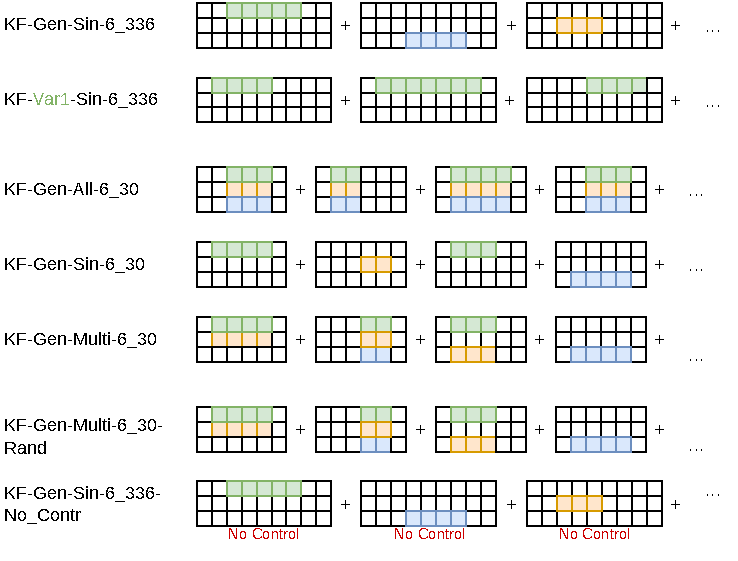
\includegraphics[width=\textwidth]{training scenarios}}
\caption{Schematic representation of gap pattern for training scenarios. Each rectangle is a data block used for training, where each row is a different variable and each column a different time. The highlighted areas represent artificial gaps. In the figure, only three variables and a small number of data points are shown. The name of the training scenarios follows this pattern: \textit{KF-\textlangle var missing\textrangle-\textlangle n var missing\textrangle-\textlangle range gap lengths\textrangle[-\textlangle modifier\textrangle]}.}
\label{fig:training}
\end{figure}

\subsection{Other methods}

The implementation of the MDS used in the results comparison is from \textsf{REddyProc} \cite{wutzler_basic_2018}. This package has been used because it provides an R interface, that can be easily integrated with Python. Conversely, \textsf{ONEFlux} implements only a C interface, whose integration in Python is significantly more challenging.  The MDS algorithm in \textsf{REddyProc} and \textsf{ONEFlux} are fully equivalent. In detail, the function \verb|REddyProc::sEddyProc_sMDSGapFill| was used, with the default settings of using \vv{SW\_IN}, \vv{TA} and \vv{VPD} as drivers with a tolerance of 2.5 \si{^\circ C}, 50 \si{W/m^s} and 5 \si{hPa} respectively as described in \textcite{reichstein_separation_2005-3}.
The data provided to MDS had a context of at least 90 days around the gap, as required by \textsf{REddyProc}.

The imputation using ERA-Interim was performed by using the ERA-I variables available in the FLUXNET 2015 dataset without further correction.

\subsection{Code Details and Availability}

The code for this project has been developed in Python. The main libraries used are: \textsf{PyTorch} \cite{NEURIPS2019_9015} for the model,  \textsf{FastAI} \cite{howard_fastai_2020} for model training and data preparation, \textsf{Altair} \cite{VanderPlas2018,Satyanarayan2017} for plotting and \textsf{Pandas} and \textsf{Polars} for data analysis. The source code and the trained model are available at \url{https://github.com/mone27/meteo_imp}, and the documentation of the library at \url{https://mone27.github.io/meteo_imp/lib}.
% \pagebreak

\section{Results}

\subsection{Correlation characteristics of meteorological variables}

\begin{figure}
\centering
\begin{subfigure}{\textwidth}
    \centering
    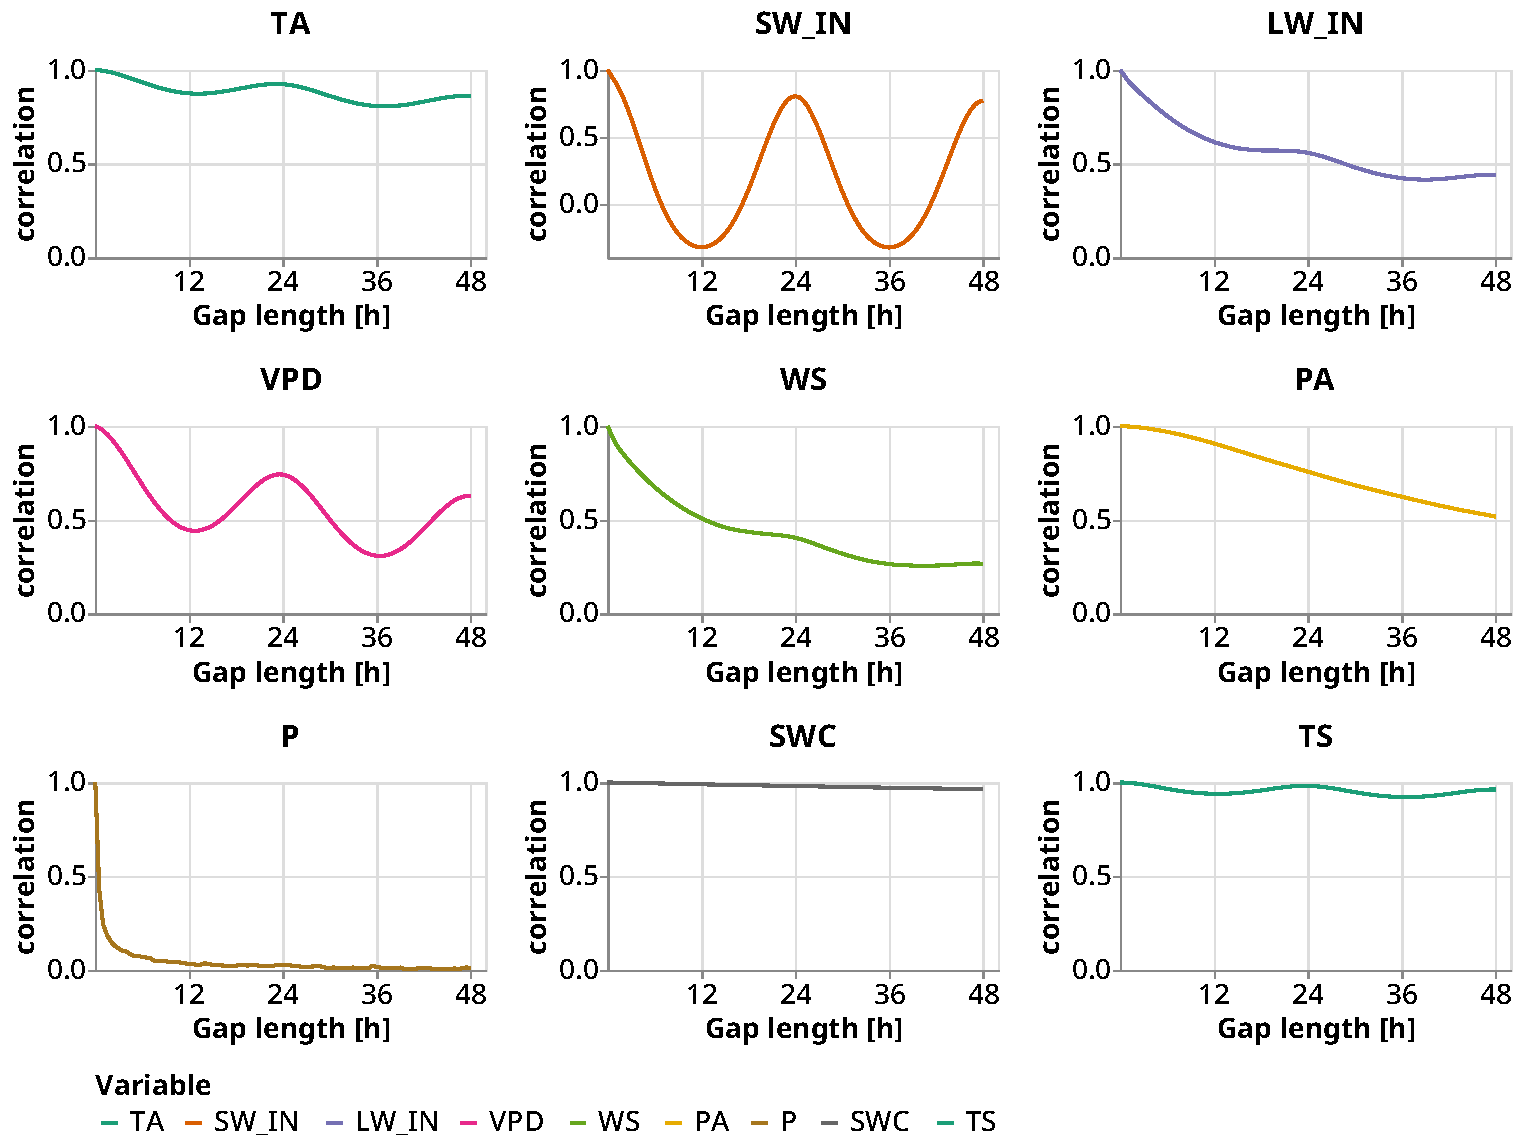
\includegraphics[width=4.5in]{temporal_autocorrelation}
    \caption{Temporal autocorrelation}%
    \label{fig:temp_autocorr}
\end{subfigure}
\begin{subfigure}{\textwidth}
        \centering%
        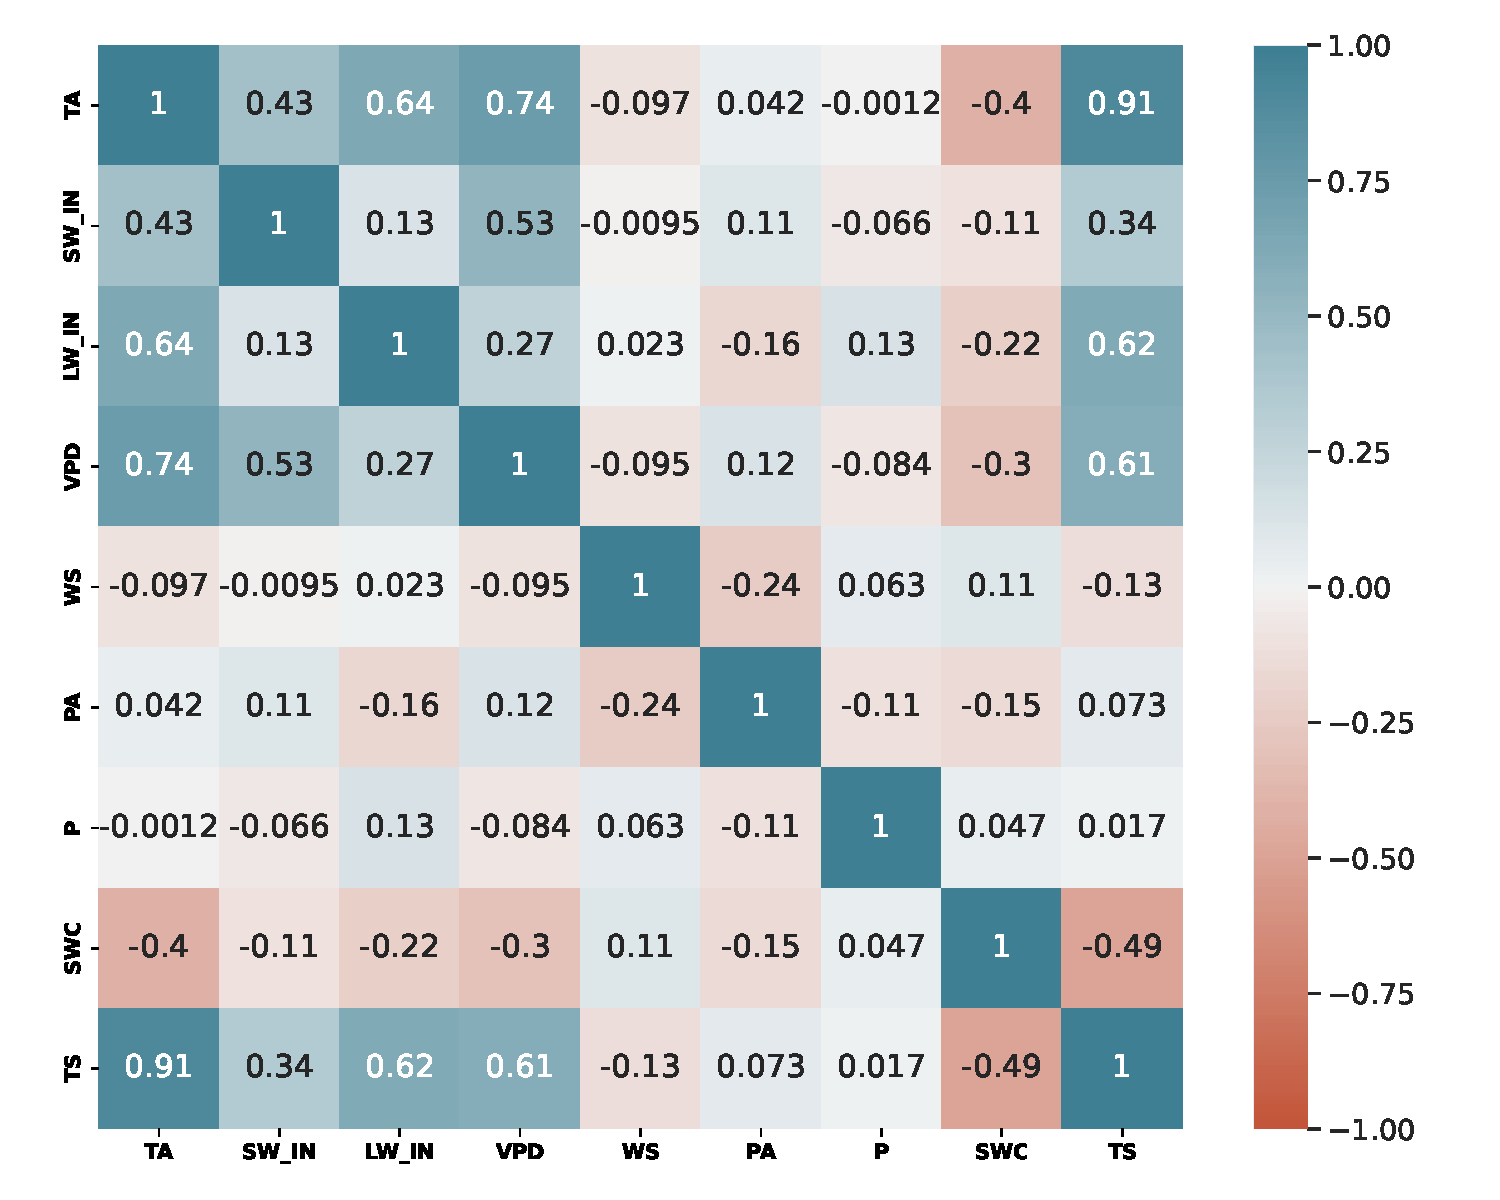
\includegraphics[width=4in]{correlation}%
        \caption{Inter-variable correlation}%
        \label{fig:corr}%
\end{subfigure}
\caption{Temporal autocorrelation (a) and inter-variable correlation (b) of meteorological variables.  Abbreviations: Air Temperature \texttt{TA}, Incoming Shortwave Radiation \texttt{SW\_IN}, Incoming Longwave Radiation \texttt{LW\_IN}, Vapor Pressure Deficit \texttt{VPD}, Wind Speed \texttt{WS}, Air Pressure \texttt{PA}, Precipitation \texttt{P}, Soil Temperature \texttt{TS}, Soil Water Content \texttt{SWC}.}
    \label{fig:correlation}
\end{figure}

The analysis of the patterns in the variable temporal autocorrelation and inter-variable correlation supports the interpretation of the results on the performance of imputation methods, as it highlights which mechanisms are available to the models to impute each variable.

The temporal autocorrelation, for a lag up to 48 hours, is shown in Figure \ref{fig:temp_autocorr}. Overall, the meteorological variables have a high temporal autocorrelation, that decreases with the lag. The only exception is the Precipitation (\vv{P}), which has a very low temporal autocorrelation. Moreover, several variables (i.e. Air Temperature \texttt{TA}, Incoming Shortwave Radiation \texttt{SW\_IN},  Vapor Pressure Deficit \texttt{VPD}, Soil Temperature \texttt{TS}) have a daily pattern with the highest temporal autocorrelation for lags that are multiple of 24 hours and the lowest for lags that are multiple of 12 hours. This is particularly evident in \vv{SW\_IN}, that has a negative correlation for a lag of 12 hours.

The variable with the highest correlation with other variable is \vv{TA} (Figure \ref{fig:corr}), which is correlated with five other variables (correlation coefficient bigger than 0.4).
\vv{TS} is highly correlated with the air temperature, thus follows a similar pattern.
Four variables: \texttt{SW\_IN} \texttt{LW\_IN}, \texttt{VPD}, \vv{SWC} have the correlation ranging between 0.4 and 0.6 with at least two other variables,
while the remaining three variables: Wind Speed (\vv{WS}), Air Pressure (\vv{PA}) and Precipitation (\vv{P}), have a low correlation with other variables.


\subsection{Comparison to other imputation methods}

The Kalman Filter (KF) has an overall better imputation performance than the state-of-the-art imputation methods: ERA-I and MDS.
In general, across all tested scenario it exhibits the same pattern: KF is the method with the smallest imputation error,
ERA-I is the second-best method while MDS is the approach with the highest imputation error (Figure \ref{fig:the_plot} and Table \ref{tbl:the_table}). The only exception is precipitation, for which the three methods are equivalent.

I compared the models by creating artificial gaps in a single variable with four different gap lengths (i.e. 6 hours, 12 hours, 1 day, 1 week).
For each combination of variable and gap length, 500 artificial gaps were generated and imputed using the three methods. The performance was measured using the RMSE (Figure \ref{fig:the_plot} and Table \ref{tbl:the_table}) and the standardized RMSE (appendix Figure \ref{fig:the_plot_stand} and Table \ref{tbl:the_table_stand}). In addition, the imputation performance was compared visually using three different example time series for all the combinations of each variable and three gap lengths: 6 hours, 12 hours and 1 week (Figures \ref{fig:ts_1-1}, \ref{fig:ts_1-2} and appendix Figures \ref{fig:ts_2-1} \ref{fig:ts_2-2}, \ref{fig:ts_3-1}, \ref{fig:ts_3-2}). For each variable, the fine-tuned KF model has been used (\textit{KF-\textlangle var\textrangle-Sin-6\_336}).

The average error reduction across all variables and gap lengths is 33\% compared to ERA-I and 57\% compared to MDS, if precipitation is excluded.
The improvement of the KF compared to ERA-I (i.e. the best performing state-of-the-art model) strongly depends on the variable analyzed and the gap length, ranging from an average of 54\% for \vv{TA} to 5\% for \vv{LW\_IN}.

Furthermore, by analyzing multiple artificial gaps for the same conditions (i.e. missing variable and gap length) the maximum value and the standard deviation of the gaps' RMSE is computed.
For virtually every scenario, the KF is the method with the smallest maximum and standard deviation of the RMSE (Figure \ref{fig:the_plot} and Table \ref{tbl:the_table}).

The imputation performance between different variable can be compared by analyzing the standardized RMSE, which measure the imputation error relative to the variable's standard deviation.
There is a wide range in imputation performance, with the standardized RMSE of the worst variable being one order of magnitude bigger of the one of the best variable.
The variables with the best imputation quality are:
Air Pressure (\vv{PA}, $\text{RMSE}_{\text{stand}} = 0.06$),
Air Temperature (\vv{TA}, $\text{RMSE}_{\text{stand}} = 0.08$) and
Soil Water Content (\vv{SWC}, $\text{RMSE}_{\text{stand}} = 0.09$).
Soil Temperature (\vv{TS} , $\text{RMSE}_{\text{stand}} = 0.14$),
Vapor Pressure Deficit (\vv{VPD}, $\text{RMSE}_{\text{stand}} = 0.17$),
Incoming Shortwave Radiation (\vv{SW\_IN}, $\text{RMSE}_{\text{stand}} = 0.25$) and
Incoming Longwave Radiation (\vv{LW\_IN}, $\text{RMSE}_{\text{stand}} = 0.33$)
have an intermediate imputation quality.
The variables with the highest imputation error are: Wind Speed (\vv{WS}, $\text{RMSE}_{\text{stand}} = 0.47$) and  Precipitation (\vv{P}, $\text{RMSE}_{\text{stand}} = 0.67$).


\begin{figure}
    \centerline{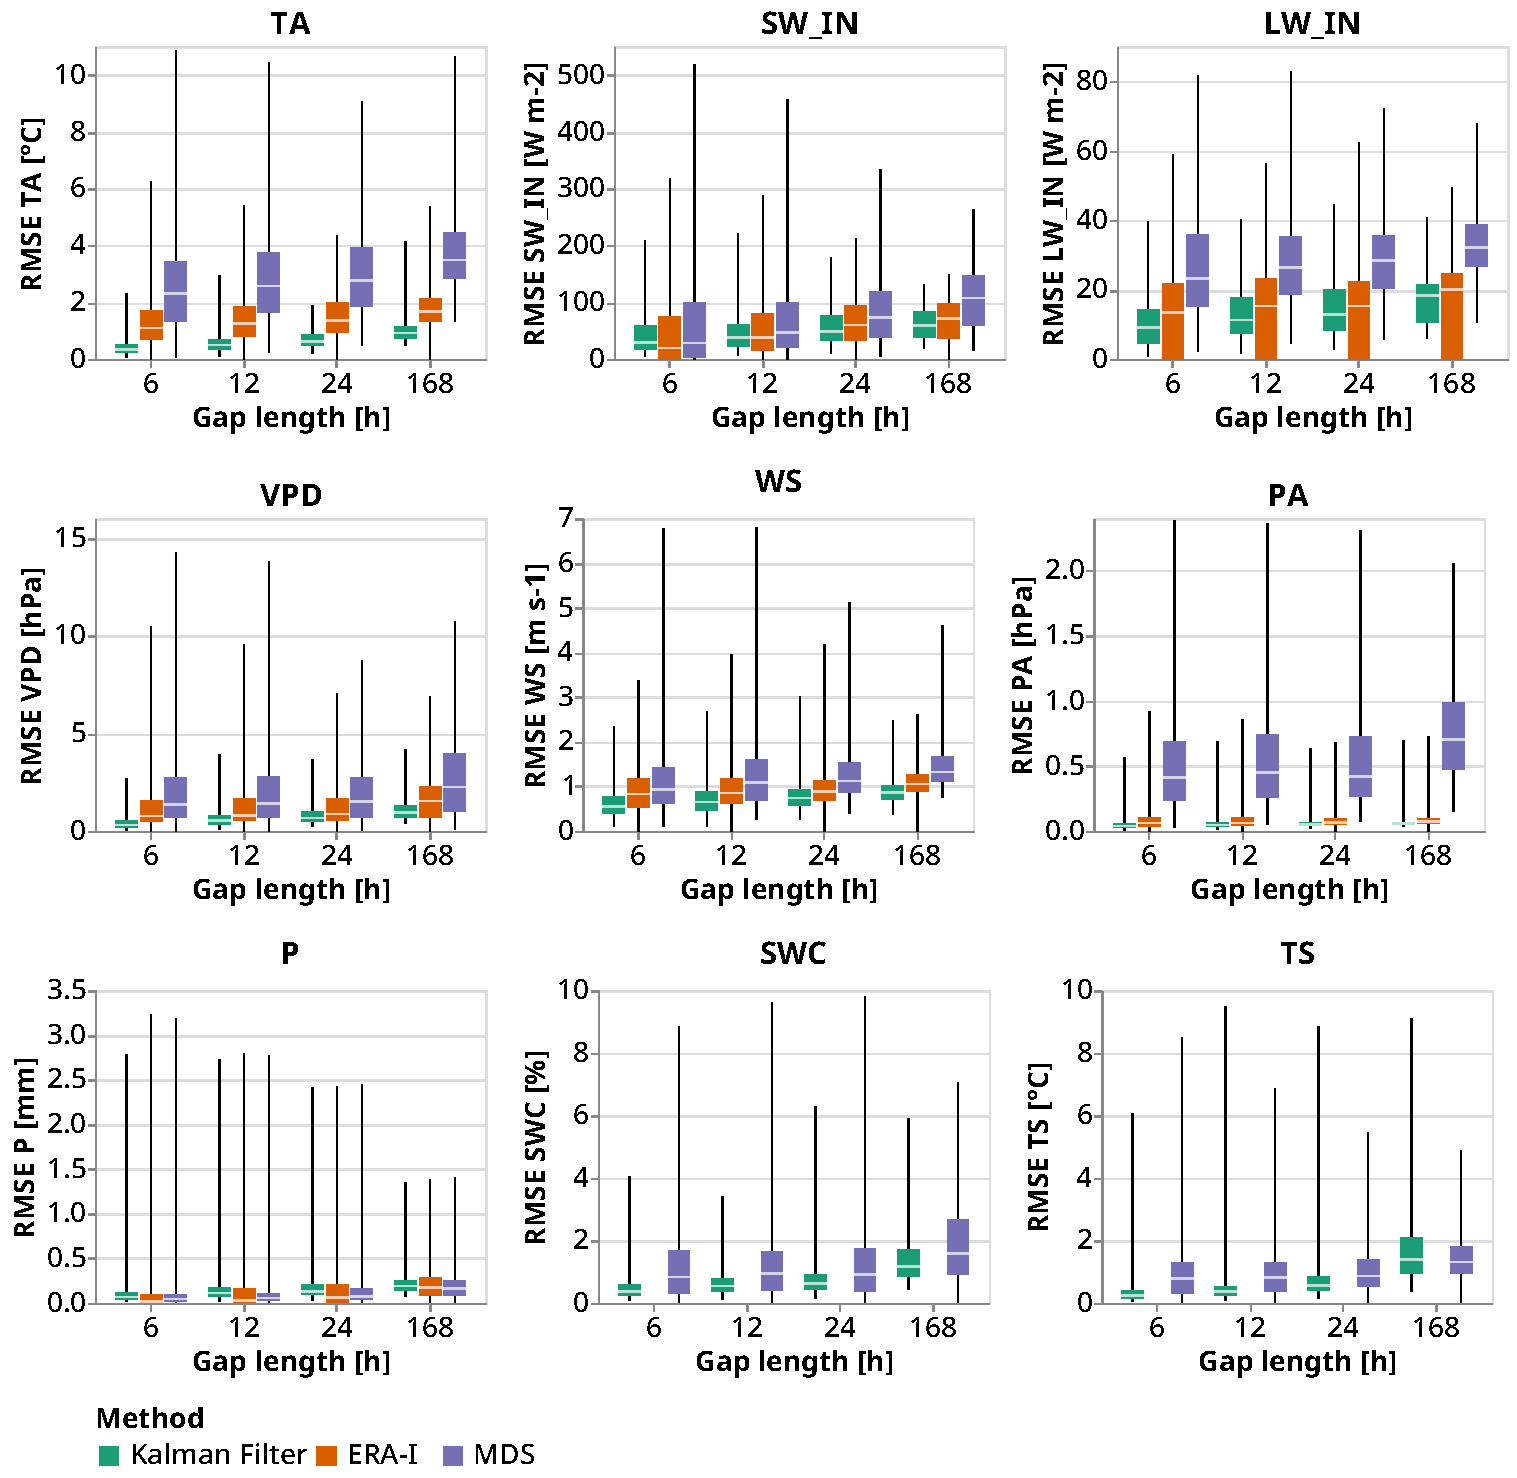
\includegraphics[width=\imgwidth]{the_plot}}
\caption{ Imputation performance of the Kalman Filter (in green) in comparison to the state-of-the-art methods: ERA-Interim (ERA-I, in orange) and Marginal Distribution Sampling (MDS, in purple). The performance was assessed by calculating for each method the \textit{Root Mean Square Error} (RMSE) for an artificial gap, with a single variable missing. For each combination of variable and gap length a sample of 500 random gaps was used (total of 18000 artificial gaps).
The KF model was fine-tuned to each variable (\textit{KF-\textlangle var\textrangle-Sin-6\_336}). ERA-I dataset does not contain \texttt{TS} and \texttt{SWC}, so it cannot be used for their imputation. The extent of the box plot vertical lines represent the maximum and minimum value of a gap RMSE.}
\label{fig:the_plot}
\end{figure}

% the tables are generated from pandas and the caption in included there, but by defining a custom command is easy to customized the caption also after
\newcommand{\CapTheTable}{Imputation performance of the Kalman filter in comparison to the state-of-the-art
methods: ERA-Interim (ERA-I) and Marginal Distribution Sampling (MDS), using mean and standard deviation of the \textit{Root Mean Square Error} (RMSE). The best method for each gap length is highlighted in bold. For each combination of gap length and variable, 500 artificial gaps were created.}
\begin{table}
\centering
\caption{RMSE Comparison imputation methods. The best method for each gap length is highligthed in bold}
\label{the_table}
\begin{tabular}{p{2.1cm}c|rr|rr|rr}
\toprule
 &  & \multicolumn{2}{r}{KalmanFilter} & \multicolumn{2}{r}{ERA} & \multicolumn{2}{r}{MDS} \\
 & RMSE & mean & std & mean & std & mean & std \\
Variable & Gap [$h$] &  &  &  &  &  &  \\
\midrule
\multirow[c]{4}{*}{\parbox{2.1cm}{\textbf{TA} [\si{°C}]}} & 6 & \bfseries 0.510 & 0.335 & 1.443 & 1.030 & 2.624 & 1.677 \\
 & 12 & \bfseries 0.685 & 0.412 & 1.347 & 0.788 & 2.665 & 1.546 \\
 & 24 & \bfseries 0.898 & 0.549 & 1.460 & 0.730 & 3.024 & 1.717 \\
 & 168 & \bfseries 1.078 & 0.561 & 1.765 & 0.714 & 3.803 & 1.232 \\
\cline{1-8}
\multirow[c]{4}{*}{\parbox{2.1cm}{\textbf{SW\_IN} [\si{W/m^2}]}} & 6 & 42.053 & 36.503 & \bfseries 41.878 & 57.449 & 56.796 & 79.190 \\
 & 12 & \bfseries 49.334 & 33.321 & 51.587 & 48.850 & 63.173 & 63.886 \\
 & 24 & \bfseries 54.067 & 26.651 & 61.879 & 38.392 & 86.693 & 63.036 \\
 & 168 & \bfseries 59.130 & 24.263 & 66.392 & 33.962 & 99.610 & 53.139 \\
\cline{1-8}
\multirow[c]{4}{*}{\parbox{2.1cm}{\textbf{LW\_IN} [\si{W/m^2}]}} & 6 & \bfseries 11.647 & 8.194 & 14.299 & 13.000 & 27.309 & 15.357 \\
 & 12 & \bfseries 14.098 & 8.483 & 15.719 & 12.606 & 29.660 & 14.269 \\
 & 24 & \bfseries 13.846 & 7.289 & 13.970 & 11.779 & 29.612 & 13.066 \\
 & 168 & 16.756 & 6.761 & \bfseries 15.921 & 11.370 & 32.895 & 8.250 \\
\cline{1-8}
\multirow[c]{4}{*}{\parbox{2.1cm}{\textbf{VPD} [\si{hPa}]}} & 6 & \bfseries 0.575 & 0.496 & 1.356 & 1.546 & 2.200 & 2.280 \\
 & 12 & \bfseries 0.897 & 0.749 & 1.352 & 1.497 & 2.027 & 2.192 \\
 & 24 & \bfseries 1.014 & 0.632 & 1.359 & 1.172 & 2.168 & 1.915 \\
 & 168 & \bfseries 1.285 & 0.799 & 1.625 & 1.111 & 2.400 & 1.898 \\
\cline{1-8}
\multirow[c]{4}{*}{\parbox{2.1cm}{\textbf{WS} [\si{m/s}]}} & 6 & \bfseries 0.585 & 0.303 & 0.894 & 0.491 & 1.194 & 0.667 \\
 & 12 & \bfseries 0.702 & 0.343 & 0.956 & 0.595 & 1.279 & 0.808 \\
 & 24 & \bfseries 0.857 & 0.385 & 1.049 & 0.510 & 1.369 & 0.794 \\
 & 168 & \bfseries 0.912 & 0.278 & 1.063 & 0.322 & 1.454 & 0.508 \\
\cline{1-8}
\multirow[c]{4}{*}{\parbox{2.1cm}{\textbf{PA} [\si{hPa}]}} & 6 & \bfseries 0.052 & 0.068 & 0.077 & 0.095 & 0.520 & 0.387 \\
 & 12 & \bfseries 0.055 & 0.056 & 0.080 & 0.072 & 0.573 & 0.434 \\
 & 24 & \bfseries 0.057 & 0.029 & 0.078 & 0.043 & 0.550 & 0.406 \\
 & 168 & \bfseries 0.065 & 0.026 & 0.083 & 0.030 & 0.770 & 0.338 \\
\cline{1-8}
\multirow[c]{4}{*}{\parbox{2.1cm}{\textbf{P} [\si{mm}]}} & 6 & \bfseries 0.100 & 0.120 & 0.105 & 0.170 & 0.101 & 0.150 \\
 & 12 & 0.125 & 0.161 & 0.131 & 0.229 & \bfseries 0.119 & 0.193 \\
 & 24 & 0.139 & 0.177 & 0.138 & 0.220 & \bfseries 0.138 & 0.217 \\
 & 168 & \bfseries 0.197 & 0.171 & 0.223 & 0.197 & 0.215 & 0.188 \\
\cline{1-8}
\multirow[c]{4}{*}{\parbox{2.1cm}{\textbf{SWC} [\si{\%}]}} & 6 & \bfseries 0.481 & 0.360 & nan & nan & 1.150 & 1.287 \\
 & 12 & \bfseries 0.605 & 0.395 & nan & nan & 1.380 & 1.629 \\
 & 24 & \bfseries 0.764 & 0.760 & nan & nan & 1.665 & 1.714 \\
 & 168 & \bfseries 1.508 & 0.982 & nan & nan & 2.023 & 1.493 \\
\cline{1-8}
\multirow[c]{4}{*}{\parbox{2.1cm}{\textbf{TS} [\si{°C}]}} & 6 & \bfseries 0.403 & 0.457 & nan & nan & 0.983 & 1.113 \\
 & 12 & \bfseries 0.613 & 0.764 & nan & nan & 0.975 & 0.844 \\
 & 24 & \bfseries 0.853 & 0.767 & nan & nan & 0.977 & 0.817 \\
 & 168 & \bfseries 1.358 & 0.697 & nan & nan & 1.507 & 0.829 \\
\cline{1-8}
\bottomrule
\end{tabular}
\end{table}


% The performance of the KF for each variable is here analyzed in detail and compared with the other methods.

\paragraph{Air Temperature} Air temperature is the variable where there is the biggest improvement in performance when using KF. It outperforms ERA-I for all gap lengths, with an average reduction in the RMSE of 54\%, while compared to MDS the reduction in RMSE is of 77\%. Comparing KF with ERA-I, the relative improvement in RMSE decrease with the gap length (69 \% for 6 hours gaps, 41\% for 1 week long gaps), while the average difference in RMSE increases with the gap length (0.29 °C  for 6 hours gaps, 0.34 °C for 1 week long gaps).
The visual inspection of the time series indicate an overall very good reconstruction of the missing data by the KF.

\paragraph{Incoming Shortwave Radiation} The KF is the method with the smaller average RMSE, but the relative improvement is small, only 12\% compared to ERA-I. The highest error is at night, where \vv{SW\_IN} is by definition always 0, but the KF often predicts sudden changes and negative values with errors in the order of 50 \si{W/m^2}. However, during the day, which is the most important condition in \vv{SW\_IN} imputation, the KF is better than other methods. This is also confirmed by visual inspections of the time series.

\paragraph{Incoming Longwave Radiation} The imputation performance of the KF is comparable with the one of ERA-I. However, KF is the best method for short gaps (20 \% improvement for 6 hours long gaps). For instance, this can be visualized in the 12 hours gap in Figure \ref{fig:ts_3-1}. The imputation performance of MDS is poor, especially for long gaps.

\paragraph{Vapor Pressure Deficit} KF is the best model for all gap lengths. The relative performance is higher for short gaps (66 \% compared to ERA-I for 6 hours long gaps) and progressively smaller for longer gaps (32 \% compared to ERA-I for 1 week long gaps). The analysis of the time series suggest that the KF is overall good at reconstructing the higher frequency changes of \vv{VPD}, but in some scenarios KF incorrectly predicts short term variation (e.g. 1 week long gap in Figure \ref{fig:ts_2-1}).

\paragraph{Wind Speed} The KF is the best imputation method for all gap lengths, with an average error reduction of 21\% compared to ERA-I. The \vv{WS} is the variable with the second highest standardized RMSE (appendix Figure \ref{fig:the_plot_stand}), which indicates that the RMSE is high compared to the \vv{WS} standard deviation. The visual inspection of the time series (Figures \ref{fig:ts_1-1} and \ref{fig:ts_2-1}), indicates that the \vv{WS} has often a high variability on short time scales, which is not captured neither by ERA-I nor by the KF.

\paragraph{Air Pressure} The imputation error of \vv{PA} is low for KF and ERA-I. The KF outperforms ERA-I with an improvement ranging from 36\% for 6 hours long gaps to 20\% for 1 week long gaps. The visual analysis of the time series suggests that the KF slightly overestimates the short term variability for \vv{PA}. MDS is significantly worse, with the imputation error one order of magnitude bigger than the one of the other methods.

\paragraph{Precipitation} The Precipitation is a variable where no method performs well, with models in some case predicting precipitation event that do not exist and in other missing the real precipitation. The RMSE of the three methods is comparable. However, the RMSE is not an accurate metric for \vv{P} imputation, due to the very high number of data points with no precipitation (over 90\% in Hainich). For reference, the RMSE of a null model (i.e. always predicts 0) is 0.28 \si{mm}, which is comparable with the errors of all imputation methods.
The visual analysis of the time series shows that ERA-I predictions are the only one that are physically realistic, even though the precipitation amount is often incorrect, while the KF often predicts negative values for \vv{P}, which is physically impossible, and MDS in a tested scenario (appendix Figure \ref{fig:ts_2-2}) predicts an unlikely constant low amount of \vv{P} for a long period.

\paragraph{Soil Water Content} The KF is the best imputation method, for short gaps there is an error reduction of 61\% compared to MDS, while for long gaps (1 week) the absolute error of the KF roughly doubles and the improvement in performance is limited to 23\%. \vv{SWC} is a variable that is not available in ERA-I, so KF and MDS are the only available methods and the KF does not have access to a control variable for \vv{SWC}.
The analysis of the time series shows that the mean of KF prediction is overall accurate, and notably it manages also to correctly predict sudden changes in \vv{SWC} (Figre \ref{fig:ts_1-2}). However, the KF constantly predicts small variations in the soil water content, which are not reflected in the observations.

\paragraph{Soil Temperature} The KF is the best imputation method for short gaps (less than 24 hours), but the MDS is better for 1 week long gaps (Figure \ref{fig:the_plot}). For short gaps there is a big difference in the methods' error (up to 60\%), but is reduced for long gaps (KF is 15\% worse than MDS for 1 week long gaps).
\vv{TS} is not available in the ERA-I dataset.
In two of the long time series analyzed the \vv{TS} is almost constant (1 week long gaps in Figure \ref{fig:ts_1-2} and \ref{fig:ts_3-2}), but the KF incorrectly predicts important variations, while the MDS is overall constant. In another scenario (appendix Figure \ref{fig:ts_2-2}), where there is a diurnal pattern in \vv{TS}, the KF predictions have an overall correct shape, even though there is roughly 1 °C error.


\newcommand{\CapTs}[2]{#1 to visualize the imputation of #2 using different methods: Kalman Filter (KF), ERA-Interim (ERA-I) and Marginal Distribution Sampling (MDS). For each variable, three random artificial gap (length 6 hours, 12 hours, 1 week) are imputed using the three methods: Kalman Filter (green), ERA-I (orange), MDS (purple).  For the KF the shaded area shows the uncertainty of the prediction $\pm 2 \sigma$ (standard deviation). The grey shaded area and the vertical black lines delimit the artificial gaps, where the observations are not available to the model but are used to assess the imputation performance. The ERA-I prediction is the control variable of the KF. The KF model has been fine-tuned to each variable (\textit{KF-\textlangle var\textrangle-Sin-6\_336}).}

\newgeometry{top=.2in}
\begin{figure}
\centerline{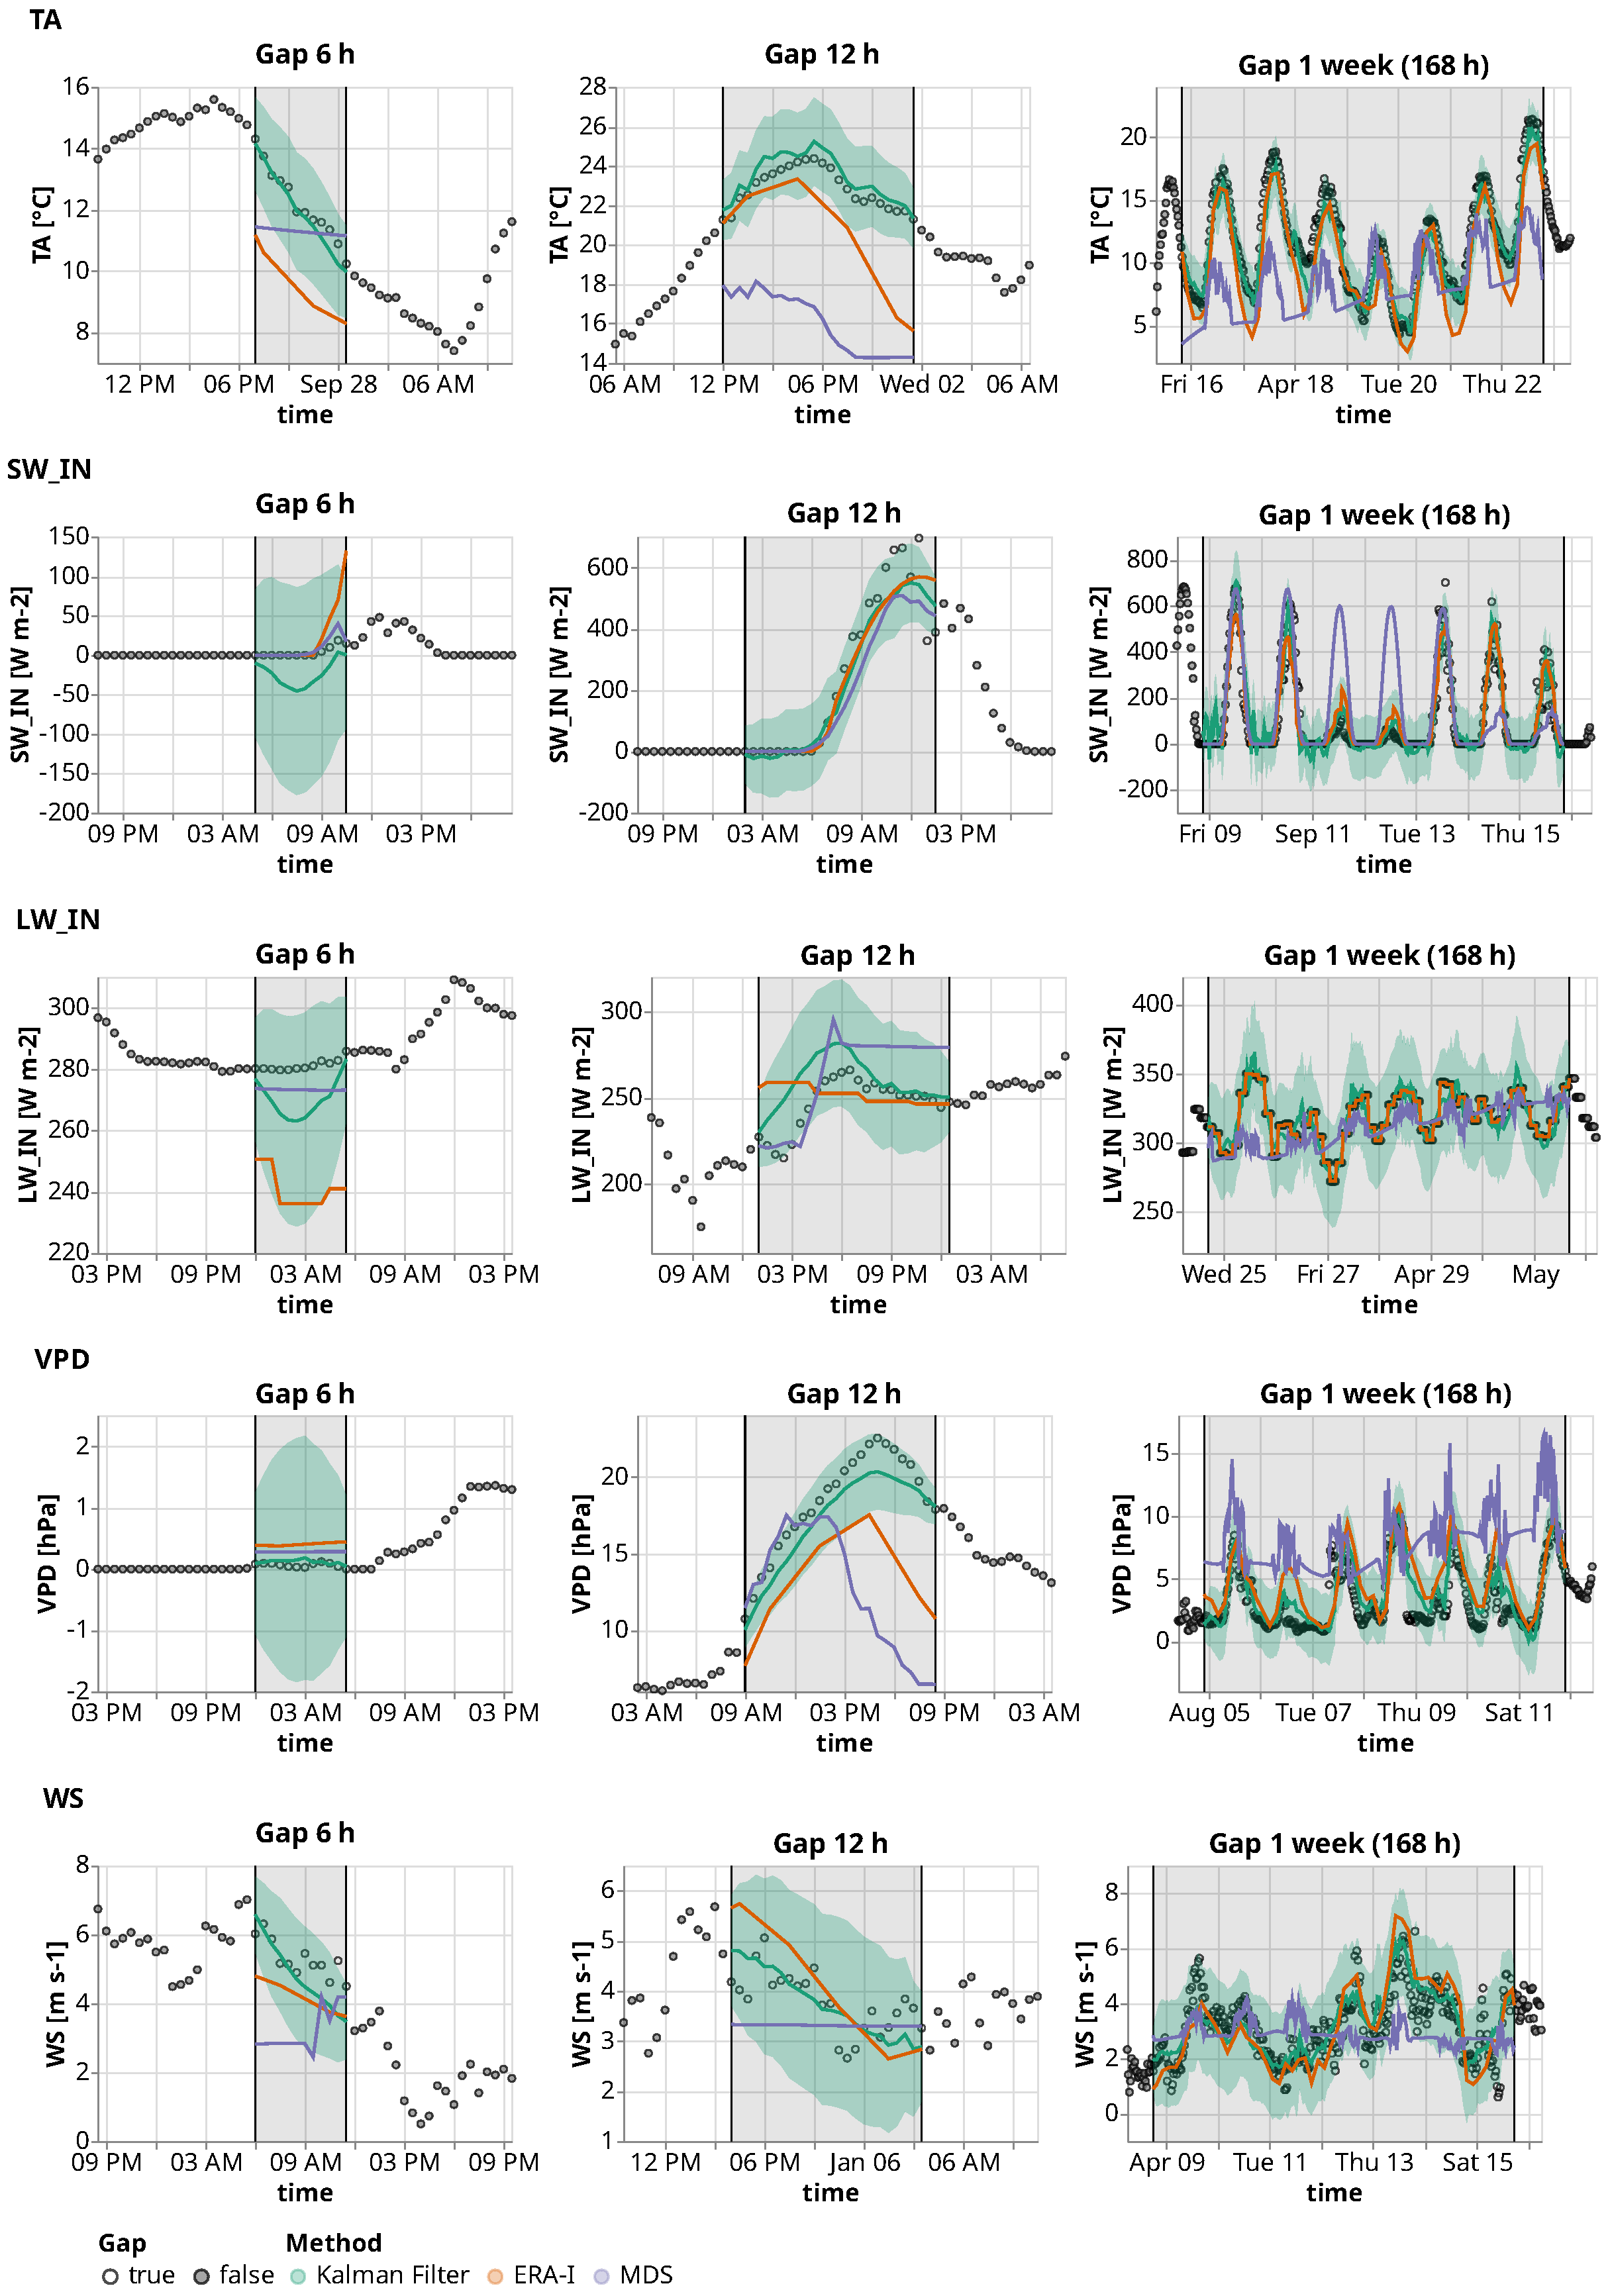
\includegraphics[width=5.7in]{timeseries_1}}
\caption{\CapTs{Time series}{\texttt{TA}, \vv{SW\_IN}, \vv{LW\_IN}, \vv{VPD}, \vv{WS}}}
\label{fig:ts_1-1}
\end{figure}
\restoregeometry

\newgeometry{top=.7in}
\begin{figure}
\centerline{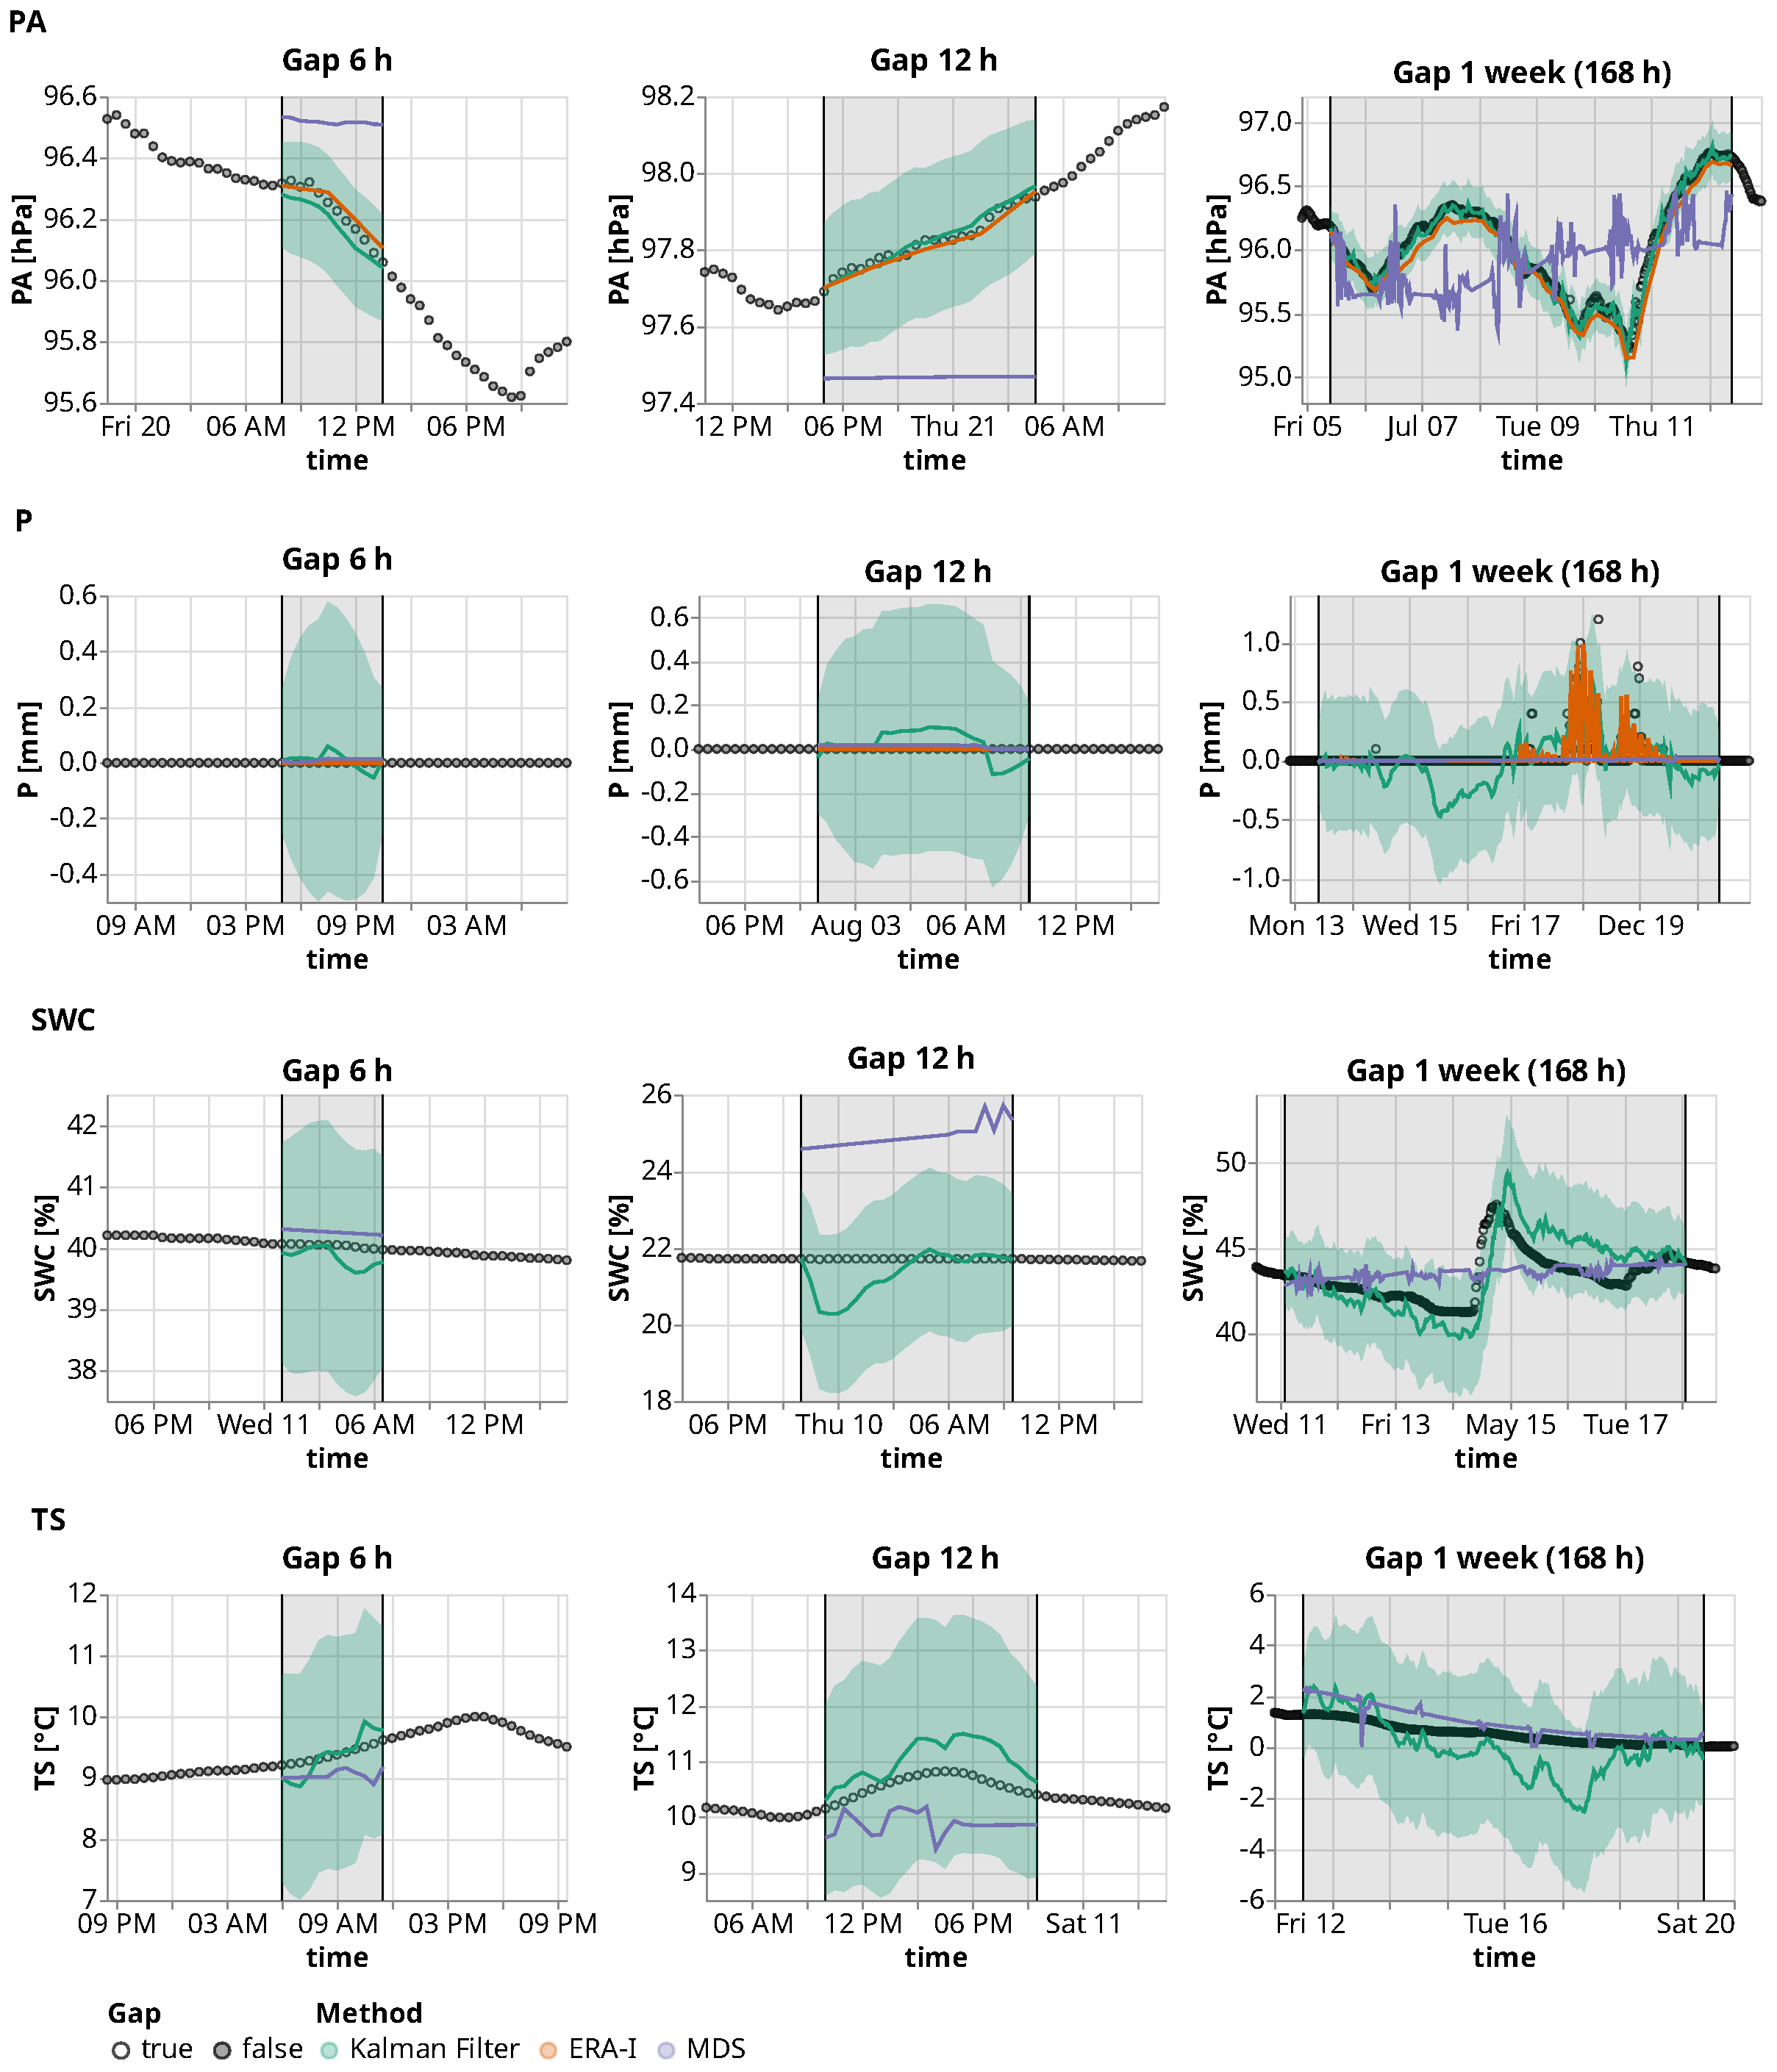
\includegraphics[width=5.7in]{timeseries_2}}
\caption{\CapTs{Time series}{\texttt{PA}, \vv{P}, \vv{SWC}, \vv{TS}}}
\label{fig:ts_1-2}
\end{figure}
\restoregeometry


\subsection{Aspects affect Kalman Filter performance}

\paragraph{Gap Length} The effect of the gap length on the KF imputation performance was analyzed by measuring the RMSE on gaps of a single variable for lengths ranging from 1 hour to 1 week (Figure \ref{fig:gap_len} and appendix Table \ref{gap_len}). For the majority of the variables the error increases with the gap length only up to 24 hours and then is almost constant. For three variables (\vv{P}, \vv{SWC} and \vv{TS}) the imputation error keeps increasing after 24 hours, but the rate decreases with the gap length. The highest rate of change of the imputation error is between 1 hour long gaps and 12 hours long gaps.
For all variables, there is a significant difference in the error of very short gaps (1 hour) and long gaps (1 week), on average the error for gaps 1 hour long is 31\% of the one for 1 week long gaps.
The variability in the RMSE between gaps (i.e. std in appendix Table \ref{gap_len}) increases with the gap length of the majority of the variables (i.e. \vv{TA}, \vv{VPD}, \vv{PA}, \vv{SWC}, \vv{TS}). For the other variables (i.e. \vv{SW\_IN}, \vv{LW\_IN}, \vv{WS}, \vv{P}), there is a decrease in RMSE variability with increases in gap length.

\begin{figure}
\centerline{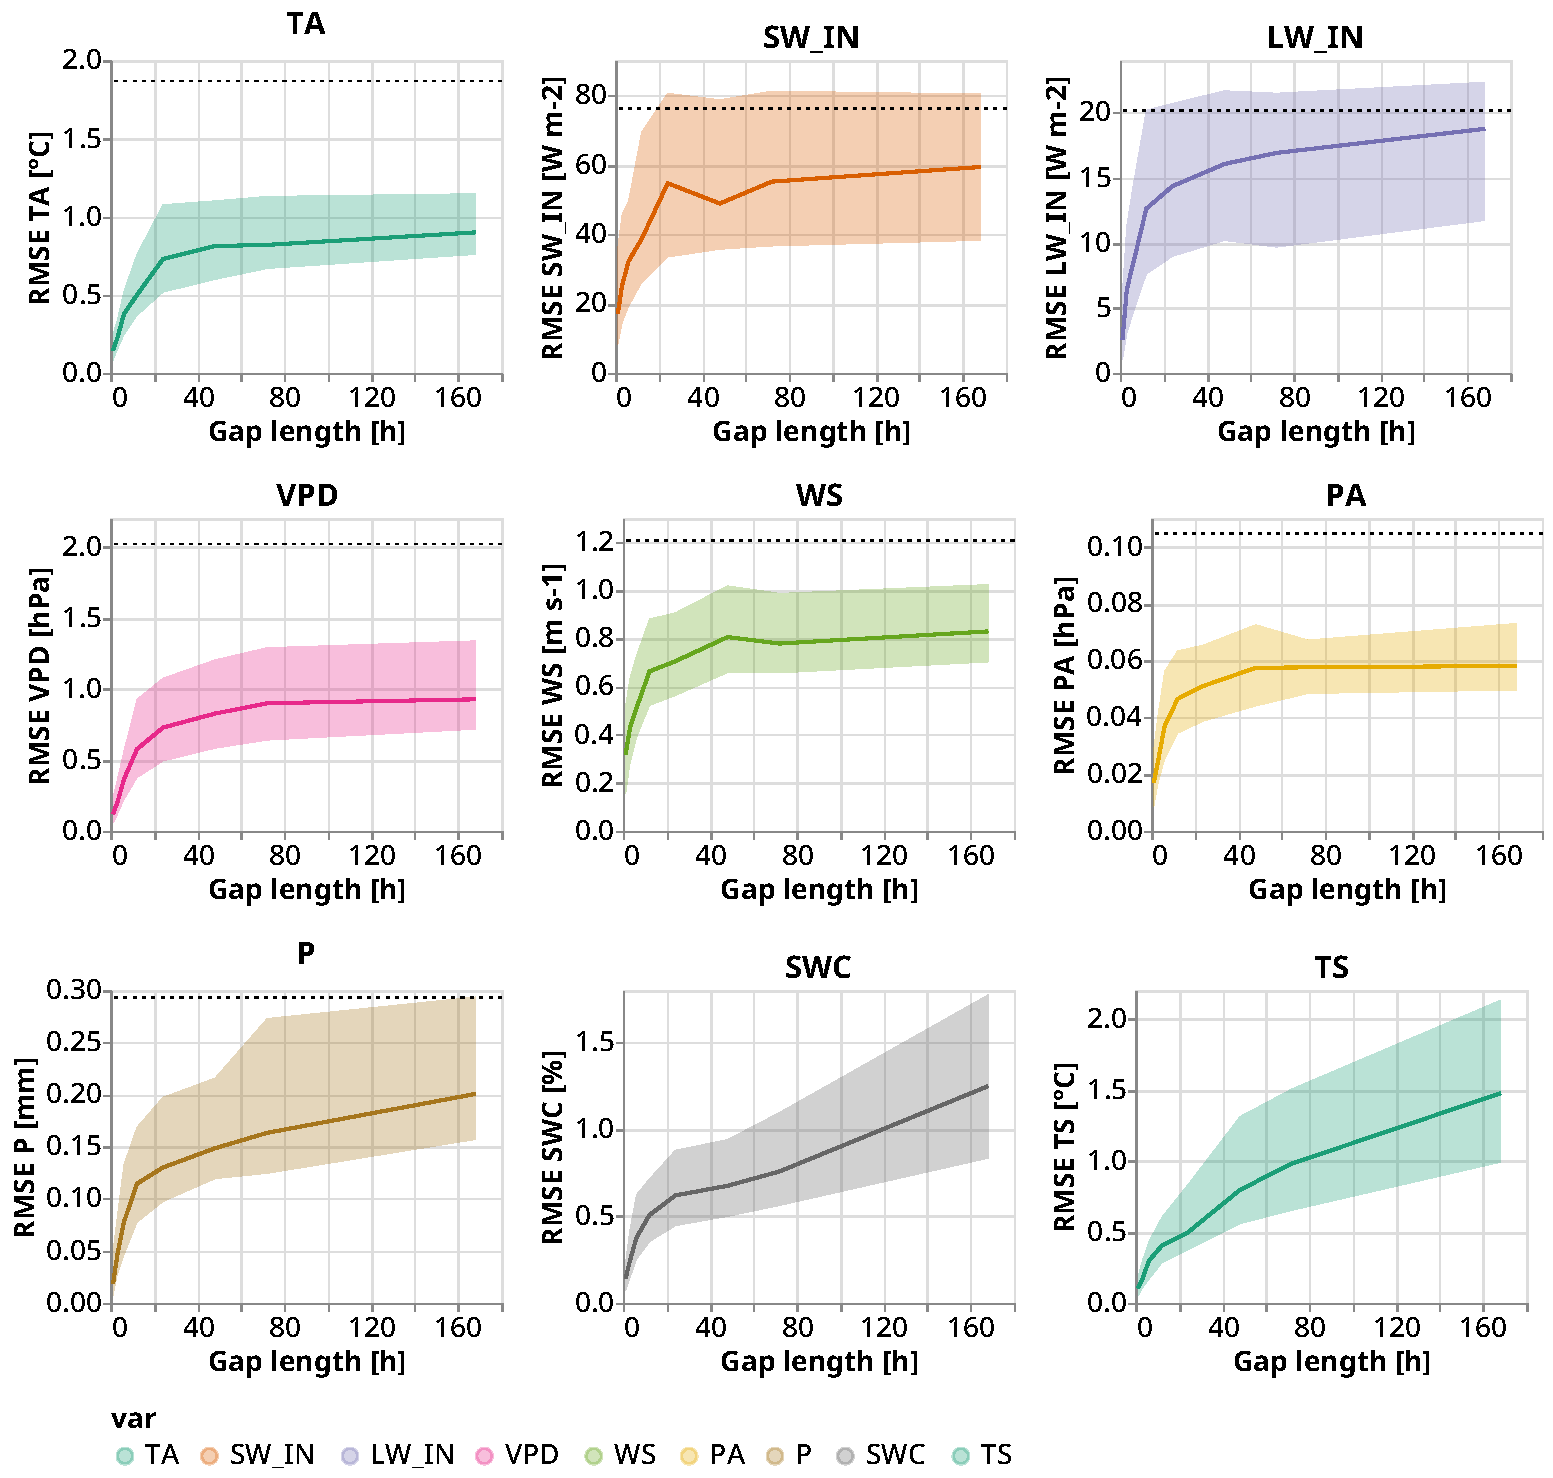
\includegraphics[width=\imgwidth]{gap_len}}
\caption{Effect of gap length on the KF performance. The solid line shows the median RMSE, while the shaded area is delimited by the first and third quartile. The dotted black line is the mean ERA-I error for the entire dataset (ERA-I data is not available for \vv{SWC} and \vv{TS}). Seven different gaps lengths were tested (1 hour, 3 hours, 6 hours, 12 hours, 1 day, 2 days, 3 days, 1 week), for each of them 500 artificial gaps were generated for every variable (total 31500 gaps). For each variable, the fine-tuned KF model has been used (\textit{KF-\textlangle var\textrangle-Sin-6\_336}).}
\label{fig:gap_len}
\end{figure}

\paragraph{Control variables}

The importance of the control variables has been assessed by comparing the imputation error of a KF model that used the control variables (\textit{KF-Gen-Sin-6\_336}) with a KF model that did not have access to the control variables (\textit{KF-Gen-Sin-6\_336-No\_Contr}). Both models were not fine-tuned for each variable.

In general, the use of control variables improves the imputation performance for all variables for all gap lengths. The exceptions are \vv{P} and \vv{TS}, where the two models are equivalent, and for short gaps (6 hours) in \vv{SWC} and \vv{WS}, where the model with the control performs worse than the one without control (Figure \ref{fig:control}).
For all variables, the longer the gap, the bigger the performance improvement of the model with the control variables (appendix Table \ref{tbl:control}).
The variable that benefits the most from the control is \vv{PA}, where for gaps 1 week long, the model without the control has an error almost 6 times bigger than the one with the control.


\begin{figure}
\centerline{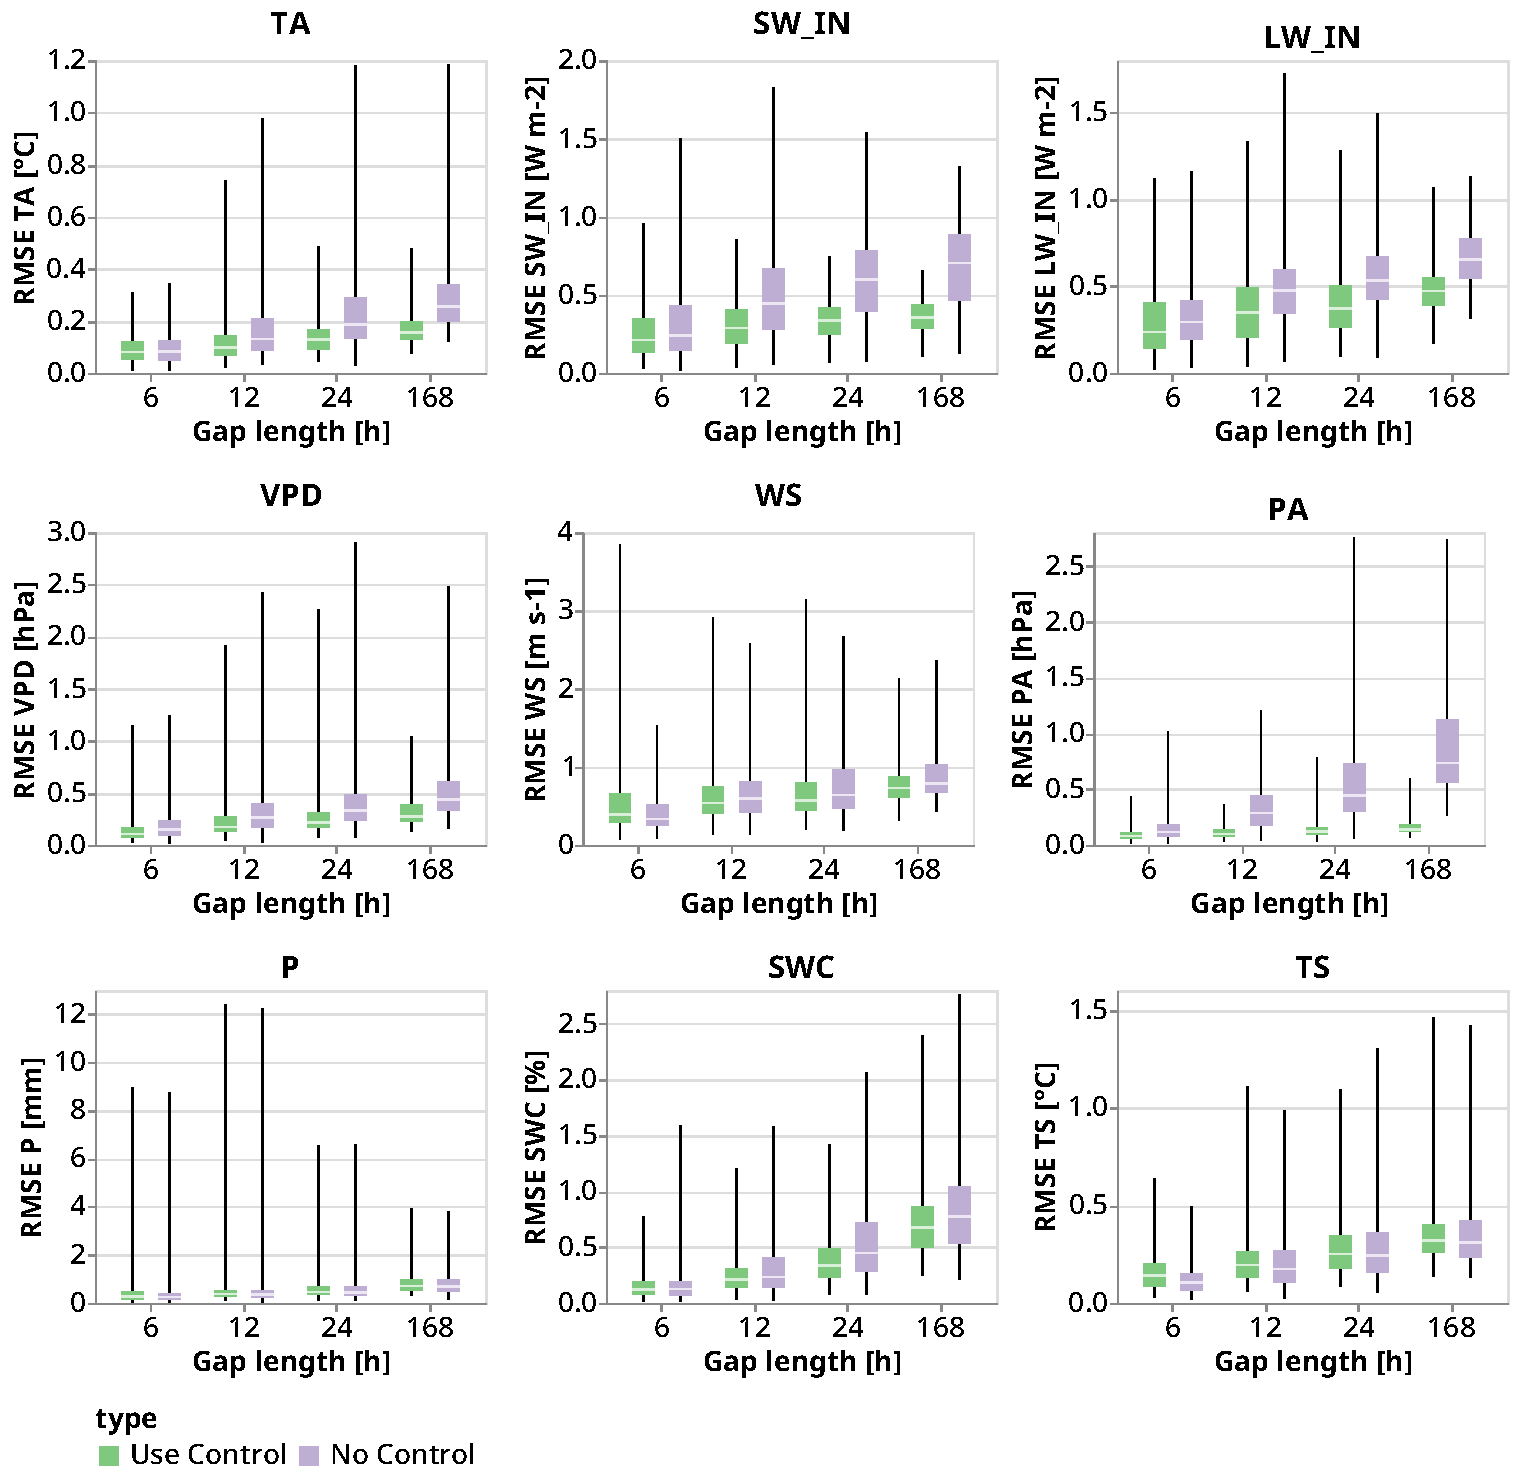
\includegraphics[width=\imgwidth]{use_control}}
\caption{Comparison of imputation performance between KF with control variables (in green, \textit{KF-Gen-Sin-6\_336}) and KF without control variables (in purple, \textit{KF-Gen-Sin-6\_336-No\_Contr}). For each combination of variable and gap length, 500 artificial gaps were created. The extent of the box plot vertical lines represent the maximum and minimum value of a gap RMSE.}
\label{fig:control}
\end{figure}

\paragraph{Gaps in multiple variables} The importance of the inter-variable correlation for the KF predictions was assessed by comparing the imputation for a gap with only one variable missing and then for the same gap with all variables missing. All the gaps were imputed using the same model (\textit{KF-Gen-Multi-6\_30}). The gap length was limited to 15 hours due to numerical stability issues.

The presence of other variables in the gap is overall improving the model predictions (Figure \ref{fig:gap_single_var} and appendix Table \ref{tbl:gap_single_var}), for some variables there is a significant error reduction (e.g. around 40 \% for \vv{TA}) but for others the improvement is minimal (e.g. less than 2\% for \vv{WS}).
Across the different variables, there is an increase in the absolute values of the difference in RMSE with an increase in gap length.

\begin{figure}
\centerline{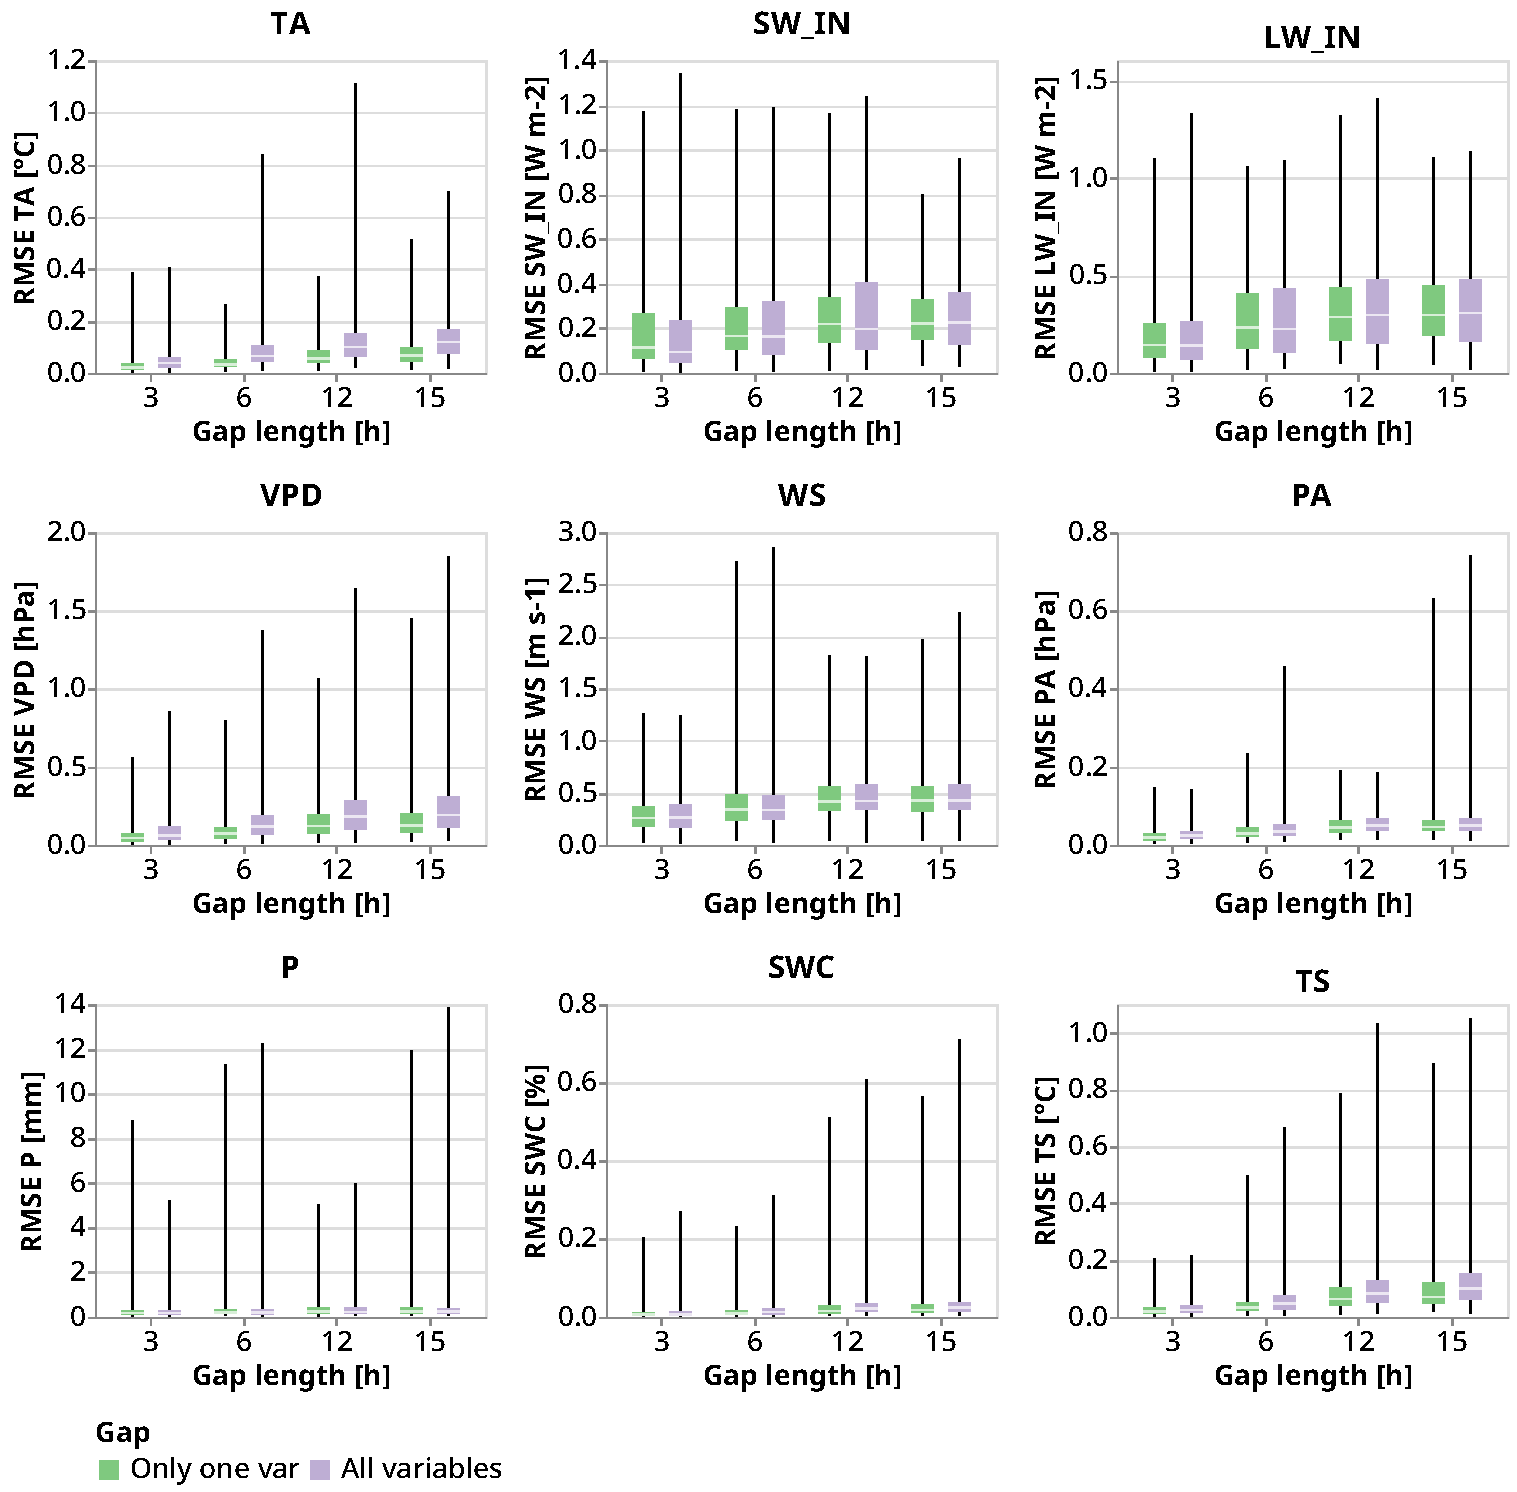
\includegraphics[width=\imgwidth]{gap_single_var}}
\caption{Comparison of imputation performance between a gap in only the variable of interest (green) and the same gap with all other variables missing (purple). The model used for imputation is always \textit{KF-Gen-Multi-6\_336}. For each combination of variable and gap length, 500 artificial gaps were created. The extent of the box plot vertical lines represent the maximum and minimum value of a gap RMSE.}
\label{fig:gap_single_var}
\end{figure}

\subsection{Kalman Filter training}

\paragraph{Variable fine-tuning} The performance of the KF is improved if the model is fine-tuned on gaps only for one variable (e.g. only for \vv{TA}).
For each variable a different model was used (\textit{KF-\textlangle var\textrangle-Sin-6\_336}) and the performance was compared to a generic model that was trained with gaps in any variable (\textit{KF-Gen-Sin-6\_336}).
% For each combination of gap length and variable, 500 artificial gaps were created.

The fine-tuning is reducing the error for all the variables (Figure \ref{fig:generic} and appendix Table \ref{tbl:generic}). The entity of the error reduction changes depending on the variable, ranging from 75\% for \vv{SWC} to 12\% for \vv{LW\_IN}.
The precipitation is the only variable that was not fine-tuned, as additional training did not improve the performance.
For the majority of variables, the variability of the RMSE between gaps of the fine-tuned model and the maximum RMSE is smaller for the fine-tuned model.

\begin{figure}
\centerline{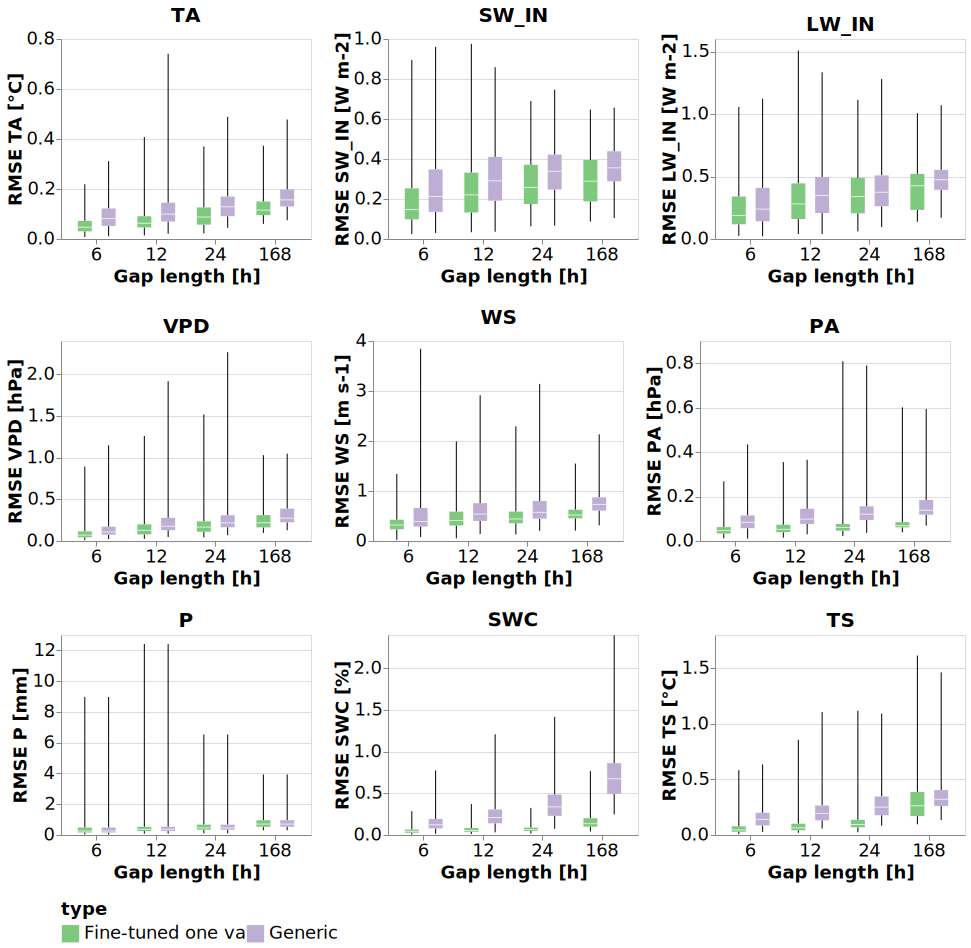
\includegraphics[width=\imgwidth]{generic}}
\caption{Comparison between KF models fine-tuned to each variable (in green, \textit{KF-\textlangle var\textrangle-Sin-6\_336}) and generic model trained for gaps in any variable (in purple, \textit{KF-Gen-Sin-6\_336}). For each combination of variable and gap length, 500 artificial gaps were created. The extent of the box plot vertical lines represent the maximum and minimum value of a gap RMSE.}
\label{fig:generic}
\end{figure}

\paragraph{Training limitations} During the training of different KF versions, I experienced limitations in the ability of the KF to learn the optimal parameters. For instance, if the KF was initialized with random parameters, it did not achieve the same performance as a KF initialized with the local trend model. The training conditions were the same, so the model that started with random parameters should have been able to learn the same parameters, but this was not the case.

The difficulties to train the KF model are shown in Figure \ref{fig:train_compare}.
Three models were compared: a model trained with gaps in multiple variables (\textit{KF-Gen-Multi-6\_336}), a model trained with gaps of only one variable (\textit{KF-Gen-Sin-6\_336}) and a model trained with gaps in multiple variables but initialized with random parameters (\textit{KF-Gen-Multi-6\_336-Rand}).
All models were trained until there was no improvement in the validation loss. The three models were used to impute a gap with only one variable was missing.
The expectation is that they should have comparable performance, but this is not the case (Figure \ref{fig:train_compare} and appendix Table \ref{tbl:train_compare}). The training conditions between \textit{KF-Gen-Multi-6\_336} and \textit{KF-Gen-Multi-6\_336-Rand} were exactly the same, so they should be able to achieve the same performance. The other model, \textit{KF-Gen-Sin-6\_336}, was trained on the same conditions that were used for testing, so it should not perform worse than \textit{KF-Multi-Sin-6\_336}.

The best model is always \textit{KF-Gen-Multi-6\_336}, while depending on variables, the second-best model is either \textit{KF-Gen-Sin-6\_336} or \textit{KF-Gen-Multi-6\_336-Rand}.

\begin{figure}
\centerline{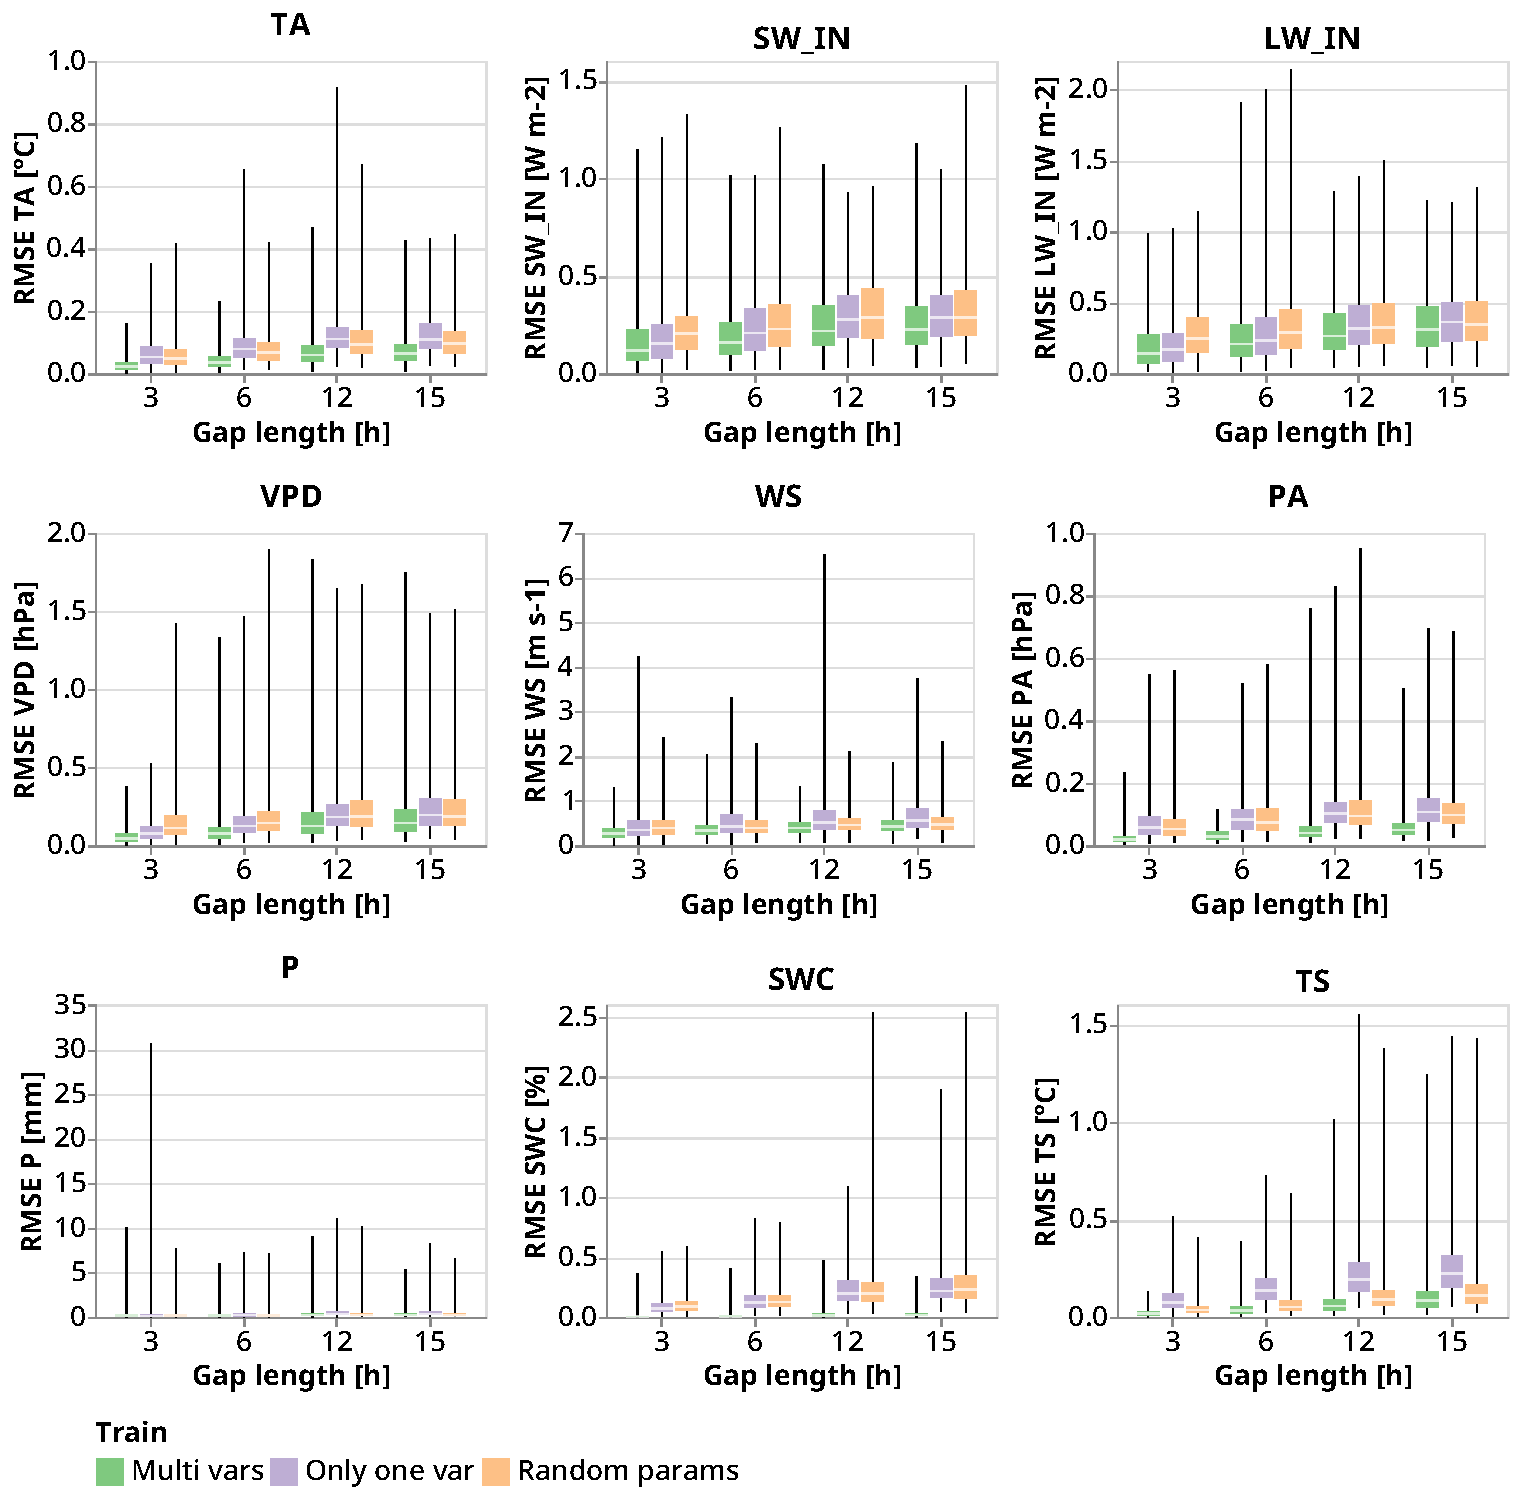
\includegraphics[width=\imgwidth]{train_compare}}
\caption{Visualization of KF training difficulties. For a gap in one variable, three models are compared: a model trained with gaps in multiple variables (in green, \textit{KF-Gen-Multi-6\_336}), a model trained with gaps of only one variable (in purple, \textit{KF-Gen-Sin-6\_336}) and a model trained with gaps in multiple variables but initialized with random parameters (in orange, \textit{KF-Gen-Multi-6\_336-Rand}). The models are expected to have comparable performances. For each combination of variable and gap length, 500 artificial gaps were created. The extent of the box plot vertical lines represent the maximum and minimum value of a gap RMSE.}
\label{fig:train_compare}
\end{figure}

\paragraph{Numerical Stability} The numerical instability of the current KF implementation limits the gap length to 15 hours long, if all the observations are missing. When only one variable is missing in a gap, I successfully tested models with a gap length of 2 weeks.
The numerical instability produces covariance matrices that are not positive definite, which in turns makes the log likelihood computation fail. The numerical stability of the filter is influenced by the values of the parameters, the observed data, the length of the gap and the total number of observations.
The Square Root KF effectively mitigates the numerical stability (appendix Figure \ref{fig:num_stab}), but results in a decrease in the runtime performance. When comparing the performance of the filtering pass, the Square Root KF is 37\% slower than the Standard KF (appendix Figure \ref{fig:num_stab_perf}), with a setting similar to the ones used in the rest of this work. The higher the number of dimensions or the batch size, the lower the relative performance of the Square Root KF.

\section{Discussion}

\subsection{Kalman Filter performance}

The KF model outperforms the state-of-the-art methods in almost every scenario tested. This result confirms the starting hypothesis that the imputation of EC meteorological time series could be improved by making a more effective use of temporal autocorrelation and by combining the imputation approaches.

The KF models the evolution of the state between consecutive time steps, thus the variable temporal autocorrelation is key for obtaining accurate predictions. The results are consistent with this: the relative performance of the KF is higher for short gaps, and the imputation error of the KF has a strong dependence on the gap length only for gaps shorter than 24 hours.  The shorter the gap, the higher the correlation between the observations close to the gap and the missing data and therefore the greater the possibility of an accurate imputation. Moreover, the relative performance of the KF is higher for variables that have a higher temporal correlation (e.g. \vv{TA}, \vv{PA} and \vv{VPD}).

When the control variables are included, the KF performance improves across all variables, confirming the hypothesis that the combination of the imputation approaches can produce better predictions. In line with the expectations, the use of the ERA-I data has an important impact on the imputation of long gaps, though it has limited influence on short gaps. Notably, the use of the control variables improve the predictions also for \vv{SWC}, even if it is not present in the ERA-I dataset.

The KF model is able to exploit the inter-variable correlation to improve the predictions. Overall, the imputation of variables with the highest correlation benefits the most from the presence of the other variables in the gaps, which matches the expectation. However, this relationship is not true for every variable. For instance, \vv{TS} has a high correlation with other variables, but I observed only a relatively small increase in performance when all the other variables were available in the gap, compared to gaps where other variables were missing.
Further, this analysis was limited to short gaps, but it is reasonable to expect that for longer gaps inter-variable correlation plays a bigger role in the KF predictions.

\subparagraph{Shortwave radiation} The low performance of the \vv{SW\_IN} at night highlights a limitation of the KF.  At its core, the KF considers only changes in the state between consecutive time steps, hence it cannot directly model the daily pattern of \vv{SW\_IN}. The KF can predict this daily change by either using other variables or the control variables. The former is not possible for \vv{SW\_IN} as it is the only variable with a very pronounced daily pattern, therefore the latter approach is the main way the KF can maintain a good imputation performance for longer gaps (see Figure \ref{fig:control}).

The limited performance of the \vv{SW\_IN} at night can also be explained by the big difference in the rate of change of \vv{SW\_IN} between the day and the night, as the KF uses constant parameters, and thus it does not consider the variability in the \vv{SW\_IN} conditions.

\subparagraph{Precipitation} The precipitation has a low temporal autocorrelation and a low correlation with other variables. Moreover, it has high temporal and spatial variability \cite{mital_sequential_2020}, especially on short time scales. In fact, ERA-I predictions have a high error for \vv{P}, which is further worsened by the temporal downscaling. The authors of the paper that introduced ERA-I for EC meteorological imputation \cite{vuichard_filling_2015}, considered the timing of the precipitation in ERA-I not accurate enough for a direct comparison of the time series.
Therefore, the poor performance of the KF is expected as none of the mechanisms used for imputations (i.e. temporal autocorrelation, inter-variable correlation and control variables) can be effectively applied to gaps in \vv{P}. 
% Furthermore, the peculiar distribution of \vv{P}, where zero is by far the most common value, further limits the potential of using the KF.

Precipitation has unique characteristics, compared to the other meteorological variables, which make it necessary to employ tailored imputation approaches. For instance, \textcite{chivers_imputation_2020} developed a method specialized in the of imputation \vv{P}, where the prediction is performed in two steps: a first model predicts whether there is going to be precipitation and a second model predicts the amount of precipitation.

\subparagraph{Wind Speed} The KF does not model accurately the high frequency variation of the wind speed. This is consistent with the limitations of ERA-I \cite{vuichard_filling_2015}. The KF cannot extract the information about the high frequency variation from other observations of the wind sped, KF is able to model higher frequency variations only if the information is present in either the control variable or in other variables. For \vv{WS}, this is not the case, as ERA-I has the same limitation and no other variable has a high correlation with the wind speed. This limitation of ERA-I is also the likely reason behind the increased error in \vv{WS} when using the control for short gap length, where the low variability in ERA-I negatively affects the model prediction.
This scenario shows one limitation arising from the simplicity of the KF compared to a Gaussian Process, which should be able to model the high frequency variation in \vv{WS}. Nonetheless, the KF has a better performance than the current imputation methods.

\paragraph{Model Training} The KF achieves the best imputation performance only when the model is fine-tuned to each variable.
Moreover, I expect that by tuning the model further to more granular conditions the performance would improve.
For instance, the rate of change of \vv{TS} is significantly  higher in a dry summer day compared to a winter day, when the ground is covered in snow. Therefore, the optimal KF parameters would be different between those conditions.
Furthermore, the optimal parameters are likely different between short gaps and long gaps, as in the first case more importance should be given to the temporal autocorrelation, while in the second case inter-variable correlation and control variables should have a bigger weight. Therefore, I expect improvements in the KF performance if the model is trained only on gaps with a similar length.
Finally, if the KF is applied to other EC sites, then it will likely require further fine-tuning, as there are different climatic conditions and the error in ERA-I data (i.e. the control variables) is a very different between EC sites \cite{vuichard_filling_2015}.

An important outcome of this work is that the KF is able to achieve good performance, but it may be difficult to learn the model parameters. The initialization of the parameters with a local trend model helped to mitigate this issue, however it is probable that the KF parameters trained in this work are still not the optimal ones. For instance, the KF performance for \vv{TS} is relatively poor for long gaps, even though it is a variable with high temporal autocorrelation and correlation with other variables, which suggest that that limiting factor is the ability to learn and not the formulation of the KF. Moreover, for short gaps, the model trained on gaps of multiple variables (i.e. in each gap a different number of variables is missing) outperforms the model trained on gaps with only one variable missing. The numerical stability issue did not allow testing this training condition on longer gaps, but it is likely that a similar pattern would be observed.


\subsection{Kalman Filter application}

The results of this study indicate that a KF can be employed to improve the imputation of meteorological variables for EC applications.
The highest error reduction is for short gaps (less than 1 day), making the KF particular suitable in this scenario. The significant improvement in the imputation of \vv{TA} is likely relevant to reduce error in Land Surface Models. Temperature is a key driver of core ecosystem processes, like photosynthesis or respiration. Those processes have a strong non-linear dependency on temperature \cite{bonan_climate_2019-2}, hence inaccuracies in the temperature estimation can have substantial impact on the Land Surface Models output.

For medium gaps (1 week) the relative performance of the KF is reduced, but it remains the best imputation approach. The \vv{TS} is the only variables where the KF has a worse performance than state-of-the-art methods.
Gaps longer than a week were not tested, but the results suggest that the predictions of the KF is going to get progressively closer to the ERA-I ones with an increase in gap length. However, for the variables not available in ERA-I the performance would probably constantly decrease with gap length.

The KF always provides an interpretable estimate of uncertainty of the predictions. The knowledge of imputation quality of each data point allows data users to make informed decisions regarding if and how to utilize the imputed data depending on each application scenario requirements.
This is a significant improvement over the use of a flag system (used in state-of-the-art methods), which is not limited to a fixed set of values.

The current KF implementation has three limitations that would prevent the application in a production scenario: numerical instability, when all variables are missing for more than 15 hours; poor performance for precipitation; physically impossible predictions of \vv{SW\_IN} at night. However, I believe that the first and third limitations are relatively straightforward to overcome, as suggested in the following section. Instead, the KF should not be used for precipitation, as it is not suited to its unique characteristics. Moreover, there is no indication that the KF can be improved to effectively predict missing precipitation.

Another aspect that needs to be considered when utilizing a KF is the necessity to fine tune the parameters.
A generic KF model, trained on a wide range of conditions, is able to impute gaps, however the best performance is achieved only when the KF parameters are fine-tuned to specific conditions.
The need to fine-tune the parameters increases the deployment complexity and potentially the computational cost.
There are different approaches to deploying a KF, ranging from using only a generic model, which is the simplest method at the cost of limited performance, to fine-tuning the model to the condition of each individual gap, which would result in the best performance while having the highest computational cost and complexity.

A promising approach is to pre-train models for different conditions (e.g. variable missing, site, time of the year), then for each gap select the KF model trained on the closest conditions. The advantages of this system are the simplicity and the computational efficiency. The  only computation overhead arises from the use of variable-specific models in gaps in multiple variables, which would require several iterations to complete the imputation when more than one variable is missing.
The main limitations of this approach are that the model parameters may be suboptimal and that it requires to train and deploy several models, one for every combination of conditions.
Moreover, if the conditions of the gap are not similar to any trained model (e.g. a different EC site), there can be a significant decrease in performance.

A variation of the approach above is to use the similarity between the training and inference condition to select a set of candidate models, instead of only one. Then each candidate model will be used to impute artificial gaps created with conditions similar to the missing data, and the model with the smallest error will be eventually employed to impute the gap. This method is better at finding the best parameters for new conditions, but it requires additional computational resources to test the different candidate models.

The last method is to fine tune the model to the conditions of each gap. This provides the best performance and flexibility at the cost of increased computational cost. Moreover, this requires the development of criteria to automatically stop the training. Furthermore, the training difficulties of the KF may prevent the parameter optimization.

The best KF deployment approach depends on the specific application (e.g. imputation of a single site or multiple sites).
% The necessity to fine-tune the KF to a specific conditions is a not critical limitation to the use of KG, but results in increased computation cost and the deployment complexity.

\subsection{Future outlook}

\paragraph{Kalman Filter improvements} This work builds the foundations for applying a KF based method for imputing meteorological variables, but further work is needed to develop this approach.
% However, further work is needed to develop a production ready model, explore potential improvements. 

As described in the previous section, there are two main issues that would prevent the use of the KF in a real world scenario.
The numerical instability of the current KF implementation limits the gaps to 15 hours, when all variables are missing.
% The current implementation is a hybrid between a square root filter and standard Kalman Filter. The use of the full covariance matrices in the smoothing pass and the in the log-likelihood computations is the source of the numerical instability.
More research is needed to develop a suitable formulation of a square root smoother, which the available literature suggests that it is possible to derive \cite{rutten_square-root_2013, park_new_1996}.
The negative predictions of \vv{SW\_IN} at night can be solved by using the KF to predict \vv{SW\_IN} during the day, and then replacing all the predictions with zero for the night. The exact time of the sunrise and sunset, and so nighttime, can be easily computed from the day of the year and the geographic coordinates.

The European Centre for Medium-Range Weather Forecasts recently released two new weather reanalysis datasets: ERA5 in 2020 \cite{hersbach_era5_2020} and ERA-5 Land  in 2021 \cite{munoz-sabater_era5-land_2021}, which supersede the ERA-Interim dataset. The ERA5-Land dataset covers only the continents, but has a much higher spatial resolution (9 km instead of 80 km) and higher temporal resolution (1 hour instead of 3 hours) compared to ERA-I. Therefore, the prediction of the KF can be improved by using ERA5-Land data instead of ERA-I as the control variable.

My analysis suggests that initial parameters have significant influence on the final parameters and thus the performance of the model. There are several approaches to initialize a KF \cite{durbin_time_2012}, and a robust comparison between the different methods may reveal a better initialization strategy than the linear trend model.

% \subparagraph{Non-linear relationships} 
The current KF implementation is limited to model only linear relationship between states and between the control and the state. There exist non-linear versions of the KF, such as the Extended Kalman Filter and the Unscented Kalman Filter \cite{dan_simon_optimal_2006}, that approximate non-linear relationship between successive states.
The relation between the ERA-I data and the observed variables is also non-linear \cite{vuichard_filling_2015}. The KF does not require linear relationship between the state and the control, so any arbitrary transformation could be applied. For instance, the use of Neural Network could be assessed. This would also integrate well with the implementation in \textsf{PyTorch} of the KF.

One parameter of the KF is the observation covariance ($R$). Currently, this parameter is estimated by the general optimization procedure, but the actual value of the observations' noise can be derived from the instrument accuracy, as the KF is a probabilistic model. This could prevent overly confident predictions.

One of the advantages of the iterative nature of the KF formulation is the ability to change the parameters between time steps.
This opens the possibility to utilize a model to predict the parameters of the KF depending on the meteorological conditions. This should overcome the necessity to fine-tune the KF parameters to each condition.
However, this may not be possible due to the difficulty of learning the parameters of the KF in the first place.

\paragraph{Model Evaluation} This study provides a first evaluation of the imputation performance of the KF, but a more in-depth analysis iss necessary to understand the real impact of applying the KF.

The first aspect to consider is that the meteorological data is not missing completely at random. Further research would be needed, but it is reasonable to assume that there is a correlation between the gaps of different variables and that the time of the year has an impact on data availability. For instance, one reason that can contribute to patterns in the missing data is that \vv{TA} and \vv{VPD} are often measured from the same sensor \cite{noauthor_associated_2020, noauthor_specification_nodate}, which increases the likelihood of both variables missing at the same time. Another scenario is a station that uses solar panels, which is more likely to have power failure during winter. A robust assessment of the imputation performance should have the pattern in artificial gaps reflecting real-world conditions.

Another aspect is to test the imputation performance using observations from different sites. EC sites are located all over the globe \cite{pastorello_fluxnet2015_2020} and the difference between climate conditions results in different patterns in the temporal autocorrelation and inter-variable correlation, which affects in turn the performance of the KF.

The metric used for the evaluation is also important. The RMSE measures the average distance between the predictions and the observations, but does not compare other characteristics of the time series such as the variance, the shape or the presence of a time-shift \cite{guen_shape_nodate}. In this study, the visual inspection of the time series was used to assess the imputation quality. This method is, however, time-consuming and is quantitative. Additional metrics, such as DILATE \cite{guen_shape_nodate}, that measure other aspect of the predictions can improve the understanding of the quality of the imputation.

Finally, the performance of the KF imputation can be evaluated by utilizing Land Surface Models (LSM). A time series with artificial gaps could be imputed using both the KF and state-of-the-art methods and then by measuring the difference in the error of the LSM compared to the original time series. This would allow to directly measure the actual impact of the improved imputation of meteorological variables.

% \pagebreak

\section{Conclusions}

The imputation of meteorological time series is necessary for EC applications. The Kalman Filter (KF) outperforms the state-of-the-art methods (ERA-I and MDS) for all variables but precipitation. The strengths of the KF are: the ability to combine different imputation approaches; the effective use of the variable temporal autocorrelation; the quantification of the predictions' uncertainty.

The imputation performance of the KF depends on the missing variable: the smallest error is for air temperature, air pressure, soil temperature and vapor pressure deficit. The air temperature is the variable with the biggest error reduction compared to state-of-the-art methods. The KF has an intermediate performance for the incoming shortwave, longwave radiation, and the wind speed. For the wind speed, the KF is limited in modelling the short term variability. The KF, like the other methods, has a poor imputation performance for the precipitation, whose unique characteristics do not make the KF a suitable method.

The current implementation of the KF is affected by numerical instability issues, which limits the model to  15 hours long gaps when all variables are missing, and at night predicts physically impossible values of the shortwave radiation. Nonetheless, both issues can be resolved by further research. However, I also identified limitations inherit in the Kalman Filter approach: the necessity to fine-tune the parameters and the difficulties to train the model. These issues do not prevent the use of the KF, but they may result in suboptimal predictions and in complex deployment setups.
% The KF requires fine-tuning to specific conditions in order to achieve the best performance, and the training may be limited by difficulties in learning the optimal model parameters.

This work shows the potential of applying the KF for EC meteorological time series imputation, however additional work is needed to further develop the imputation method and to better assess its performance. 
% \pagebreak

\printbibliography

\pagebreak

\appendix

% add separate numering for appendix
\renewcommand\thefigure{\thesection.\arabic{figure}}
\renewcommand\thetable{\thesection.\arabic{table}}
\renewcommand\theequation{\thesection.\arabic{equation}}

\FloatBarrier

\section{Additional Results}

\setcounter{figure}{0}
\setcounter{table}{0}

% \subsection{Comparison to other imputation methods}

\begin{figure}[H]
    \centerline{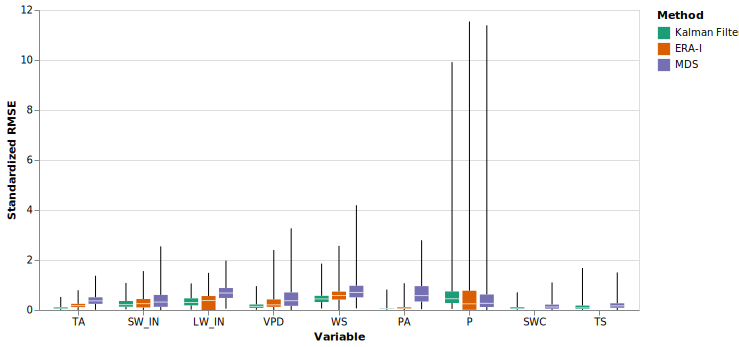
\includegraphics[width=\imgwidth]{the_plot_stand}}
\caption{Box plot to compare Standardized Root Mean Square Error(RMSE) for each variable between the different methods: Kalman Filter and the state-of-the-art methods ERA and MDS. The same data from Figure \ref{fig:the_plot} has been aggregated for all gap lengths. The extent of the box plot vertical lines represent the maximum and minimum value of a gap RMSE.}
\label{fig:the_plot_stand}
\end{figure}

\newcommand{\CapTheTableStand}{Imputation performance of the Kalman filter in comparison to the state-of-the-art
methods: ERA-Interim (ERA-I) and Marginal Distribution Sampling (MDS), using mean and standard deviation of the \textit{Root Mean Square Error} (RMSE). The best method for each gap length is highlighted in bold. For each combination of gap length and variable, 500 artificial gaps were created.}
\begin{table}
\centering
\caption{Comparison of imputation methods using Standardized RMSE. The best method for each gap length is highligthed in bold}
\label{the_table_stand}
\begin{tabular}{p{2.1cm}c|rr|rr|rr}
\toprule
 &  & \multicolumn{2}{r}{KalmanFilter} & \multicolumn{2}{r}{ERA} & \multicolumn{2}{r}{MDS} \\
 & RMSE & mean & std & mean & std & mean & std \\
Variable & Gap [$h$] &  &  &  &  &  &  \\
\midrule
\multirow[c]{4}{*}{\parbox{2.1cm}{\textbf{TA}}} & 6 & \bfseries 0.062 & 0.036 & 0.170 & 0.126 & 0.342 & 0.239 \\
 & 12 & \bfseries 0.091 & 0.057 & 0.186 & 0.114 & 0.371 & 0.221 \\
 & 24 & \bfseries 0.107 & 0.054 & 0.193 & 0.101 & 0.380 & 0.203 \\
 & 168 & \bfseries 0.136 & 0.059 & 0.221 & 0.081 & 0.477 & 0.166 \\
\cline{1-8}
\multirow[c]{4}{*}{\parbox{2.1cm}{\textbf{SW\_IN}}} & 6 & \bfseries 0.218 & 0.202 & 0.242 & 0.325 & 0.311 & 0.419 \\
 & 12 & \bfseries 0.242 & 0.170 & 0.266 & 0.244 & 0.340 & 0.338 \\
 & 24 & \bfseries 0.284 & 0.147 & 0.323 & 0.201 & 0.425 & 0.292 \\
 & 168 & \bfseries 0.308 & 0.124 & 0.344 & 0.171 & 0.526 & 0.263 \\
\cline{1-8}
\multirow[c]{4}{*}{\parbox{2.1cm}{\textbf{LW\_IN}}} & 6 & \bfseries 0.261 & 0.193 & 0.329 & 0.310 & 0.636 & 0.358 \\
 & 12 & \bfseries 0.309 & 0.201 & 0.352 & 0.300 & 0.669 & 0.321 \\
 & 24 & 0.341 & 0.198 & \bfseries 0.336 & 0.291 & 0.706 & 0.296 \\
 & 168 & 0.405 & 0.160 & \bfseries 0.390 & 0.265 & 0.785 & 0.211 \\
\cline{1-8}
\multirow[c]{4}{*}{\parbox{2.1cm}{\textbf{VPD}}} & 6 & \bfseries 0.133 & 0.104 & 0.297 & 0.354 & 0.477 & 0.492 \\
 & 12 & \bfseries 0.190 & 0.142 & 0.290 & 0.295 & 0.489 & 0.480 \\
 & 24 & \bfseries 0.219 & 0.141 & 0.286 & 0.236 & 0.438 & 0.367 \\
 & 168 & \bfseries 0.294 & 0.168 & 0.380 & 0.258 & 0.609 & 0.450 \\
\cline{1-8}
\multirow[c]{4}{*}{\parbox{2.1cm}{\textbf{WS}}} & 6 & \bfseries 0.372 & 0.191 & 0.561 & 0.313 & 0.699 & 0.482 \\
 & 12 & \bfseries 0.432 & 0.207 & 0.588 & 0.323 & 0.776 & 0.490 \\
 & 24 & \bfseries 0.484 & 0.205 & 0.584 & 0.275 & 0.785 & 0.374 \\
 & 168 & \bfseries 0.582 & 0.208 & 0.670 & 0.214 & 0.920 & 0.379 \\
\cline{1-8}
\multirow[c]{4}{*}{\parbox{2.1cm}{\textbf{PA}}} & 6 & \bfseries 0.056 & 0.046 & 0.088 & 0.072 & 0.621 & 0.516 \\
 & 12 & \bfseries 0.064 & 0.052 & 0.090 & 0.068 & 0.659 & 0.500 \\
 & 24 & \bfseries 0.072 & 0.047 & 0.092 & 0.060 & 0.651 & 0.473 \\
 & 168 & \bfseries 0.079 & 0.056 & 0.098 & 0.063 & 0.904 & 0.449 \\
\cline{1-8}
\multirow[c]{4}{*}{\parbox{2.1cm}{\textbf{P}}} & 6 & \bfseries 0.398 & 0.905 & 0.404 & 1.126 & 0.420 & 1.090 \\
 & 12 & 0.480 & 0.887 & 0.495 & 1.060 & \bfseries 0.465 & 1.004 \\
 & 24 & \bfseries 0.558 & 0.865 & 0.591 & 1.029 & 0.566 & 0.946 \\
 & 168 & \bfseries 0.697 & 0.625 & 0.795 & 0.720 & 0.767 & 0.705 \\
\cline{1-8}
\multirow[c]{4}{*}{\parbox{2.1cm}{\textbf{SWC}}} & 6 & \bfseries 0.057 & 0.041 & - & - & 0.147 & 0.175 \\
 & 12 & \bfseries 0.068 & 0.049 & - & - & 0.143 & 0.148 \\
 & 24 & \bfseries 0.085 & 0.065 & - & - & 0.152 & 0.165 \\
 & 168 & \bfseries 0.179 & 0.141 & - & - & 0.219 & 0.167 \\
\cline{1-8}
\multirow[c]{4}{*}{\parbox{2.1cm}{\textbf{TS}}} & 6 & \bfseries 0.066 & 0.059 & - & - & 0.169 & 0.157 \\
 & 12 & \bfseries 0.108 & 0.114 & - & - & 0.177 & 0.155 \\
 & 24 & \bfseries 0.162 & 0.130 & - & - & 0.191 & 0.151 \\
 & 168 & \bfseries 0.248 & 0.141 & - & - & 0.254 & 0.135 \\
\cline{1-8}
\bottomrule
\end{tabular}
\end{table}

% \subsection{Additional Time series}

\newgeometry{top=.2in}
\begin{figure}
\centerline{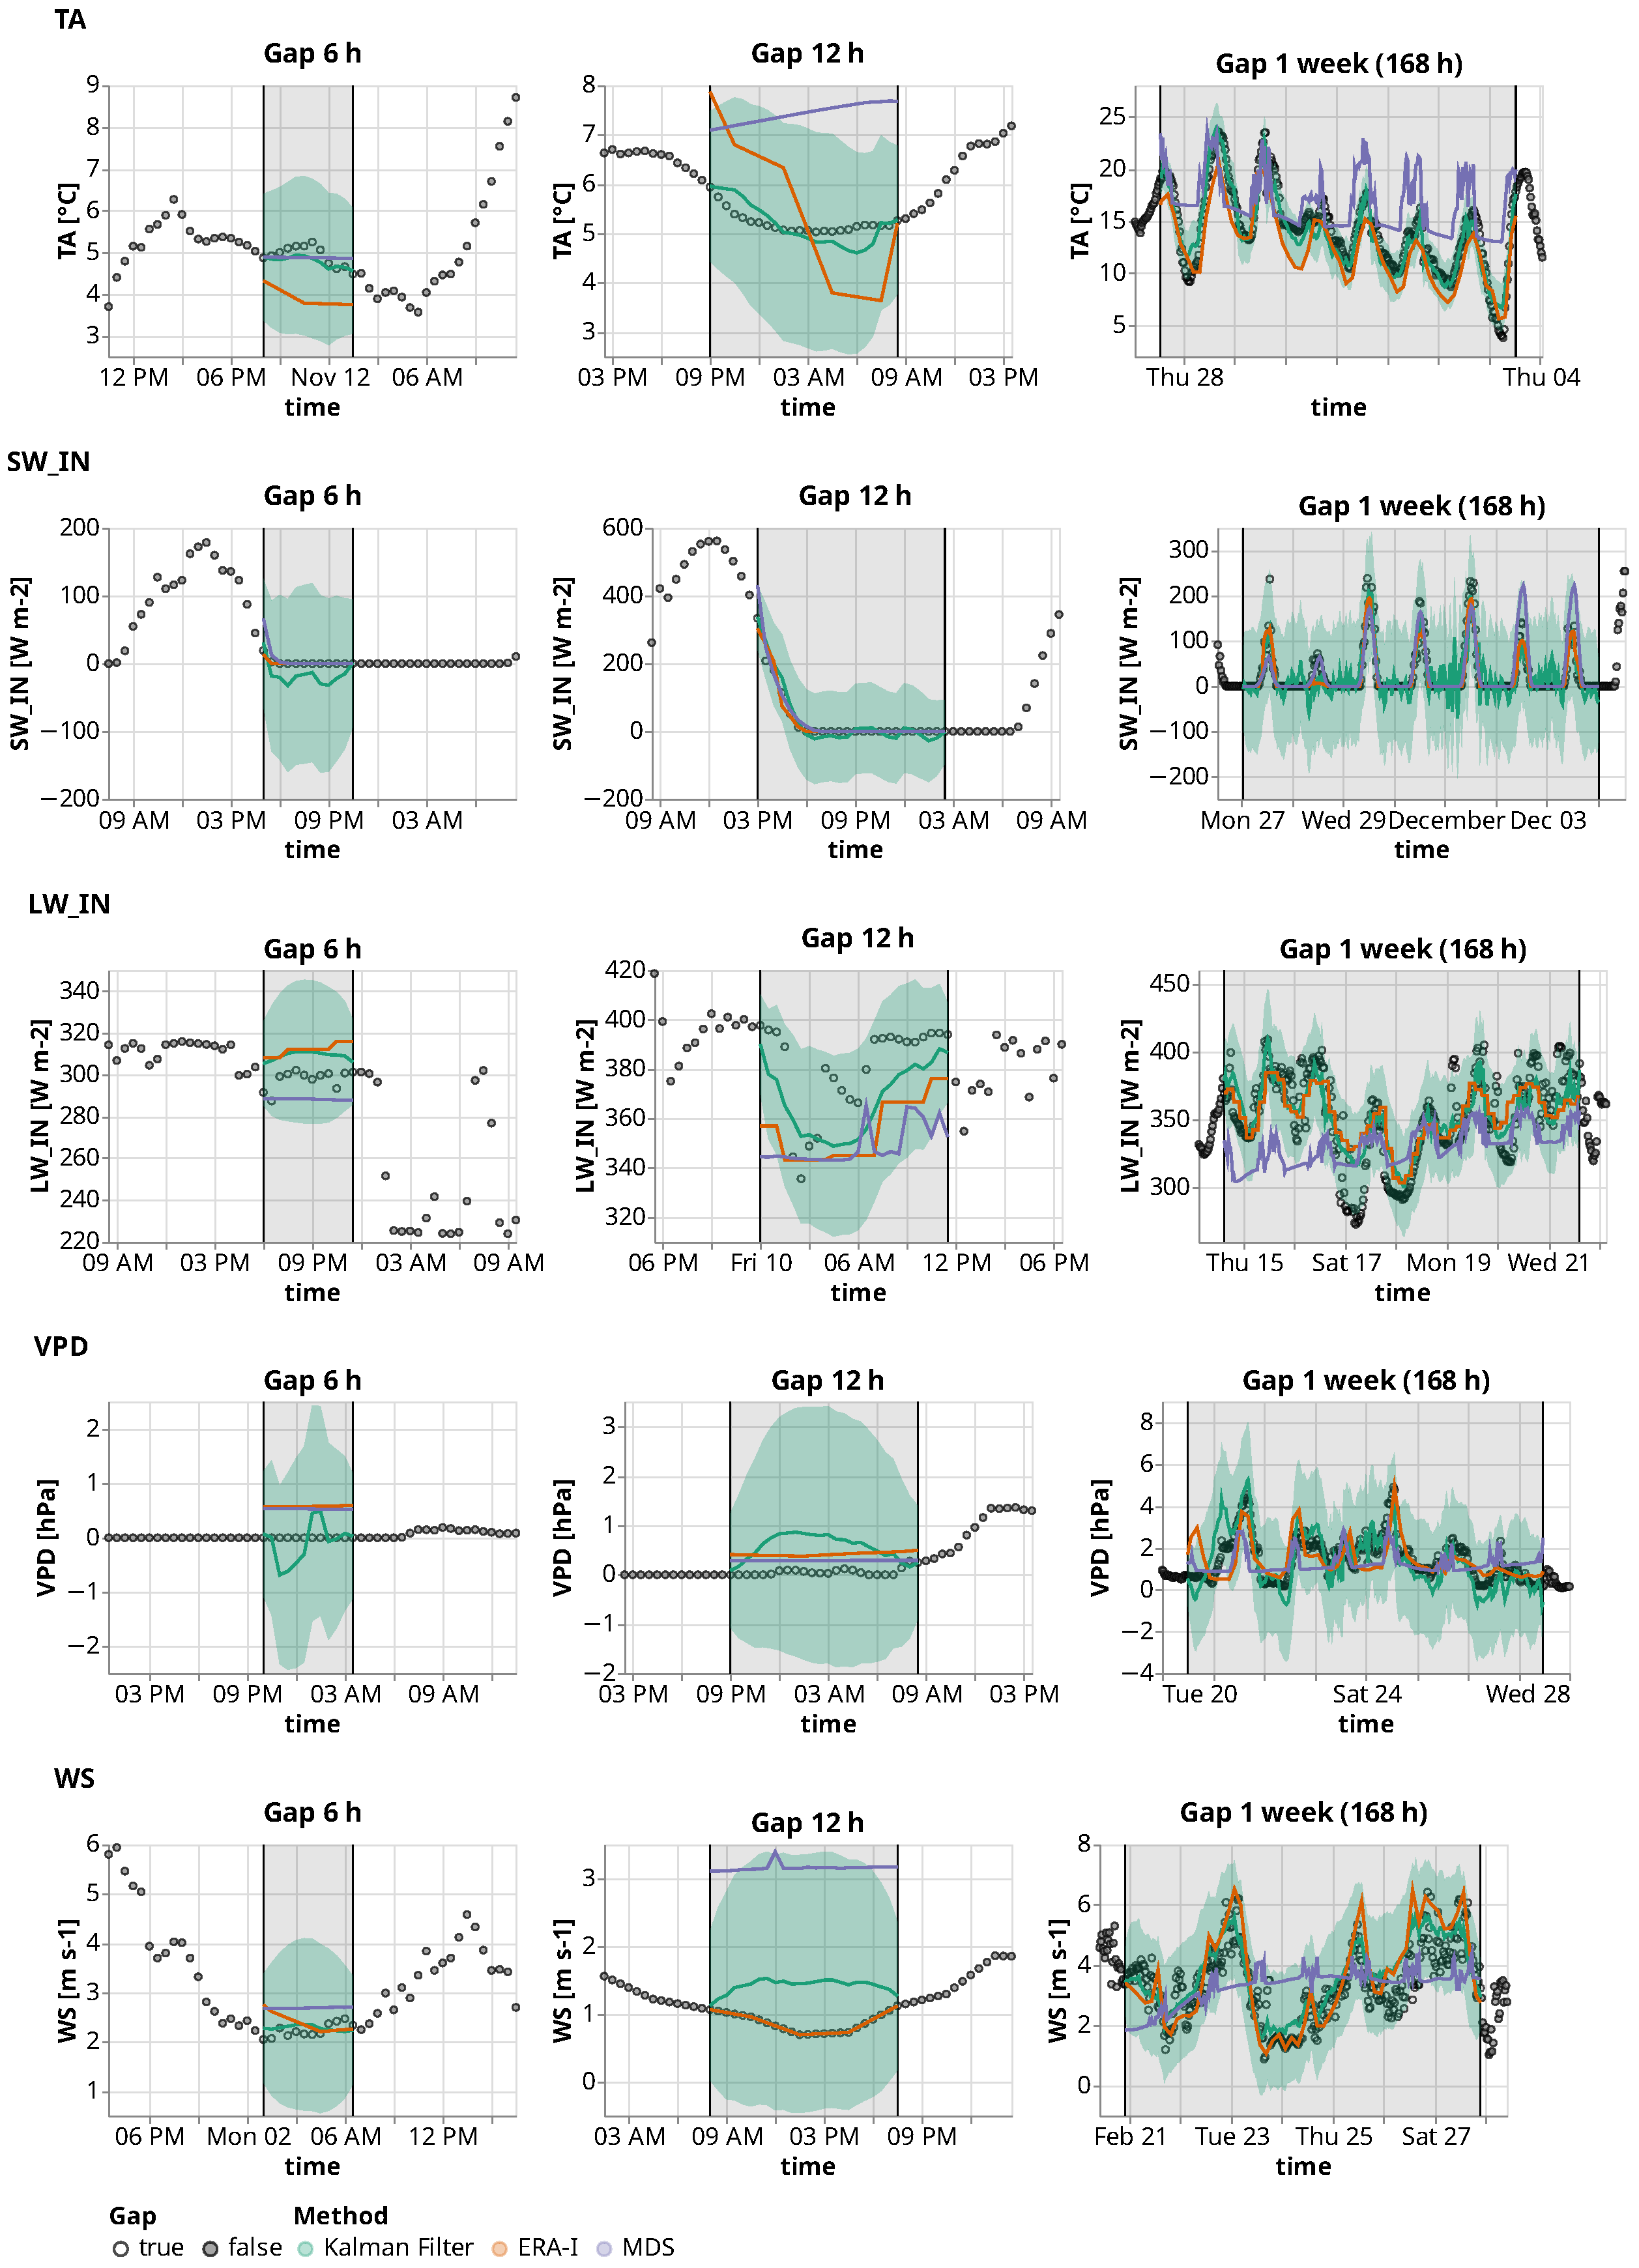
\includegraphics[width=5.7in]{timeseries_1_1}}
\caption{\CapTs{Second time series}{\texttt{TA}, \vv{SW\_IN}, \vv{LW\_IN}, \vv{VPD}, \vv{WS}}}
\label{fig:ts_2-1}
\end{figure}

\newgeometry{top=.7in}
\begin{figure}
\centerline{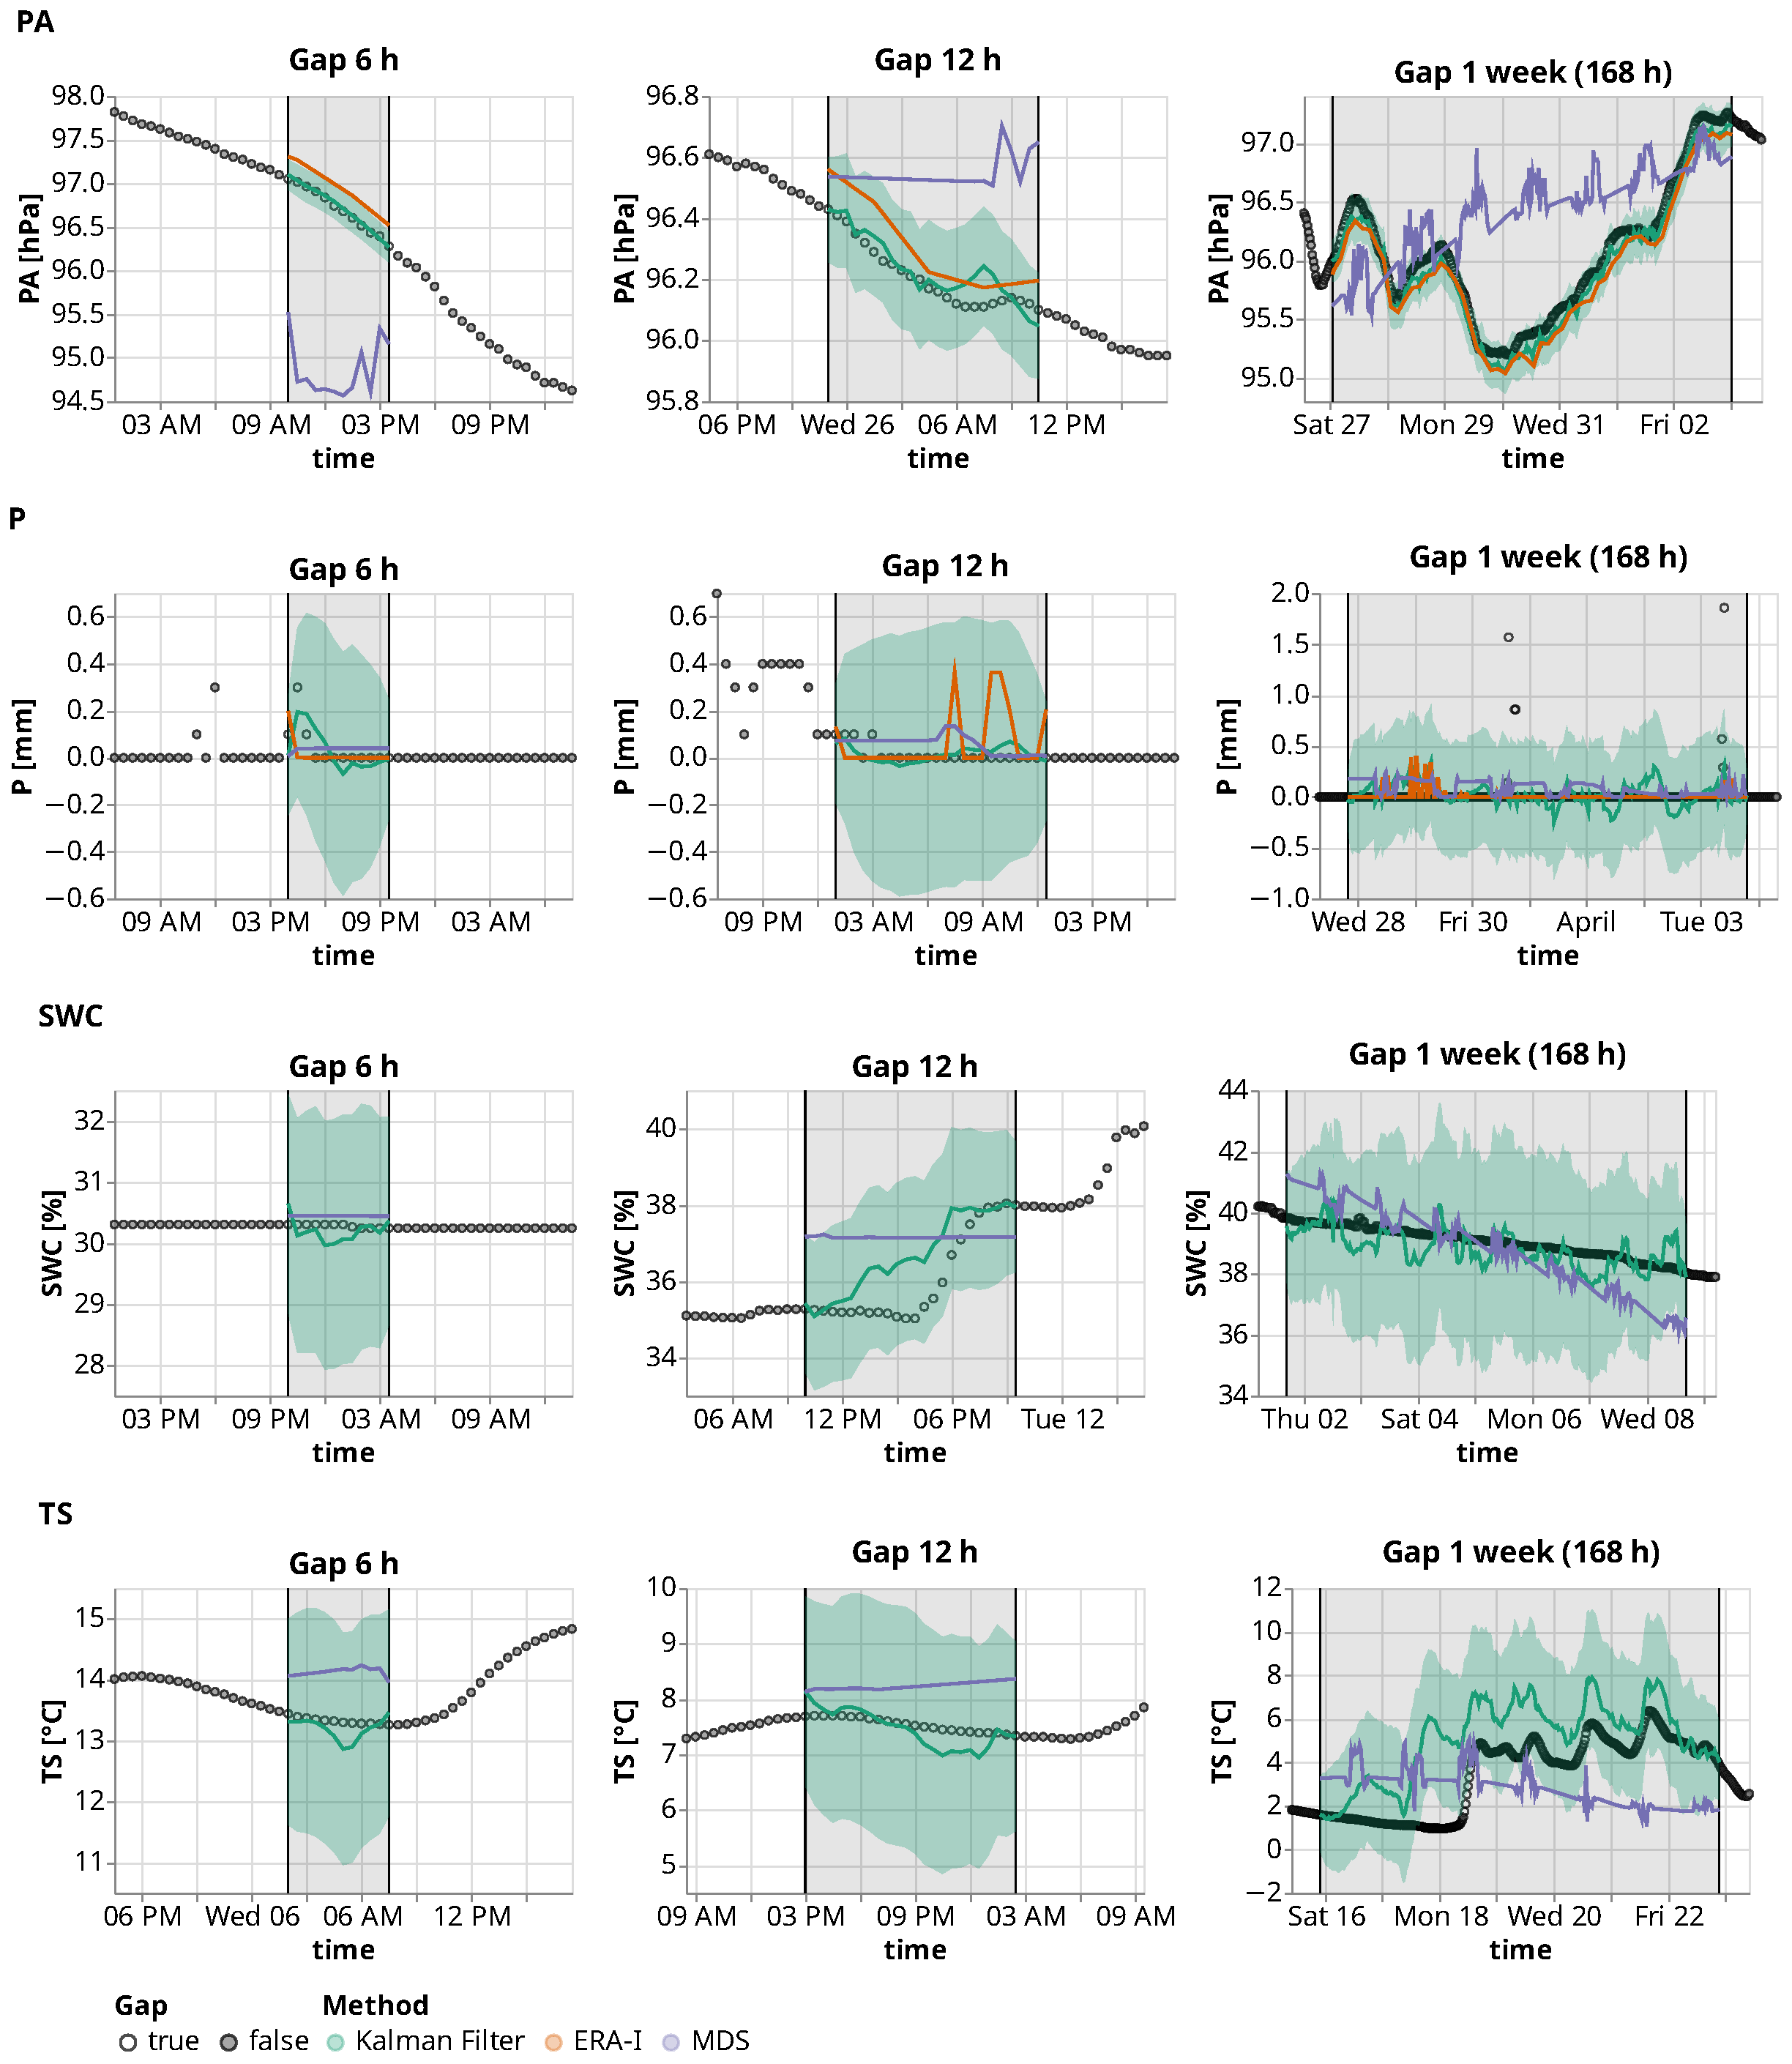
\includegraphics[width=\imgwidth]{timeseries_2_1}}
\caption{\CapTs{Second time series}{\texttt{PA}, \vv{P}, \vv{SWC}, \vv{TS}}}
\label{fig:ts_2-2}
\end{figure}

\newgeometry{top=.2in}
\begin{figure}
\centerline{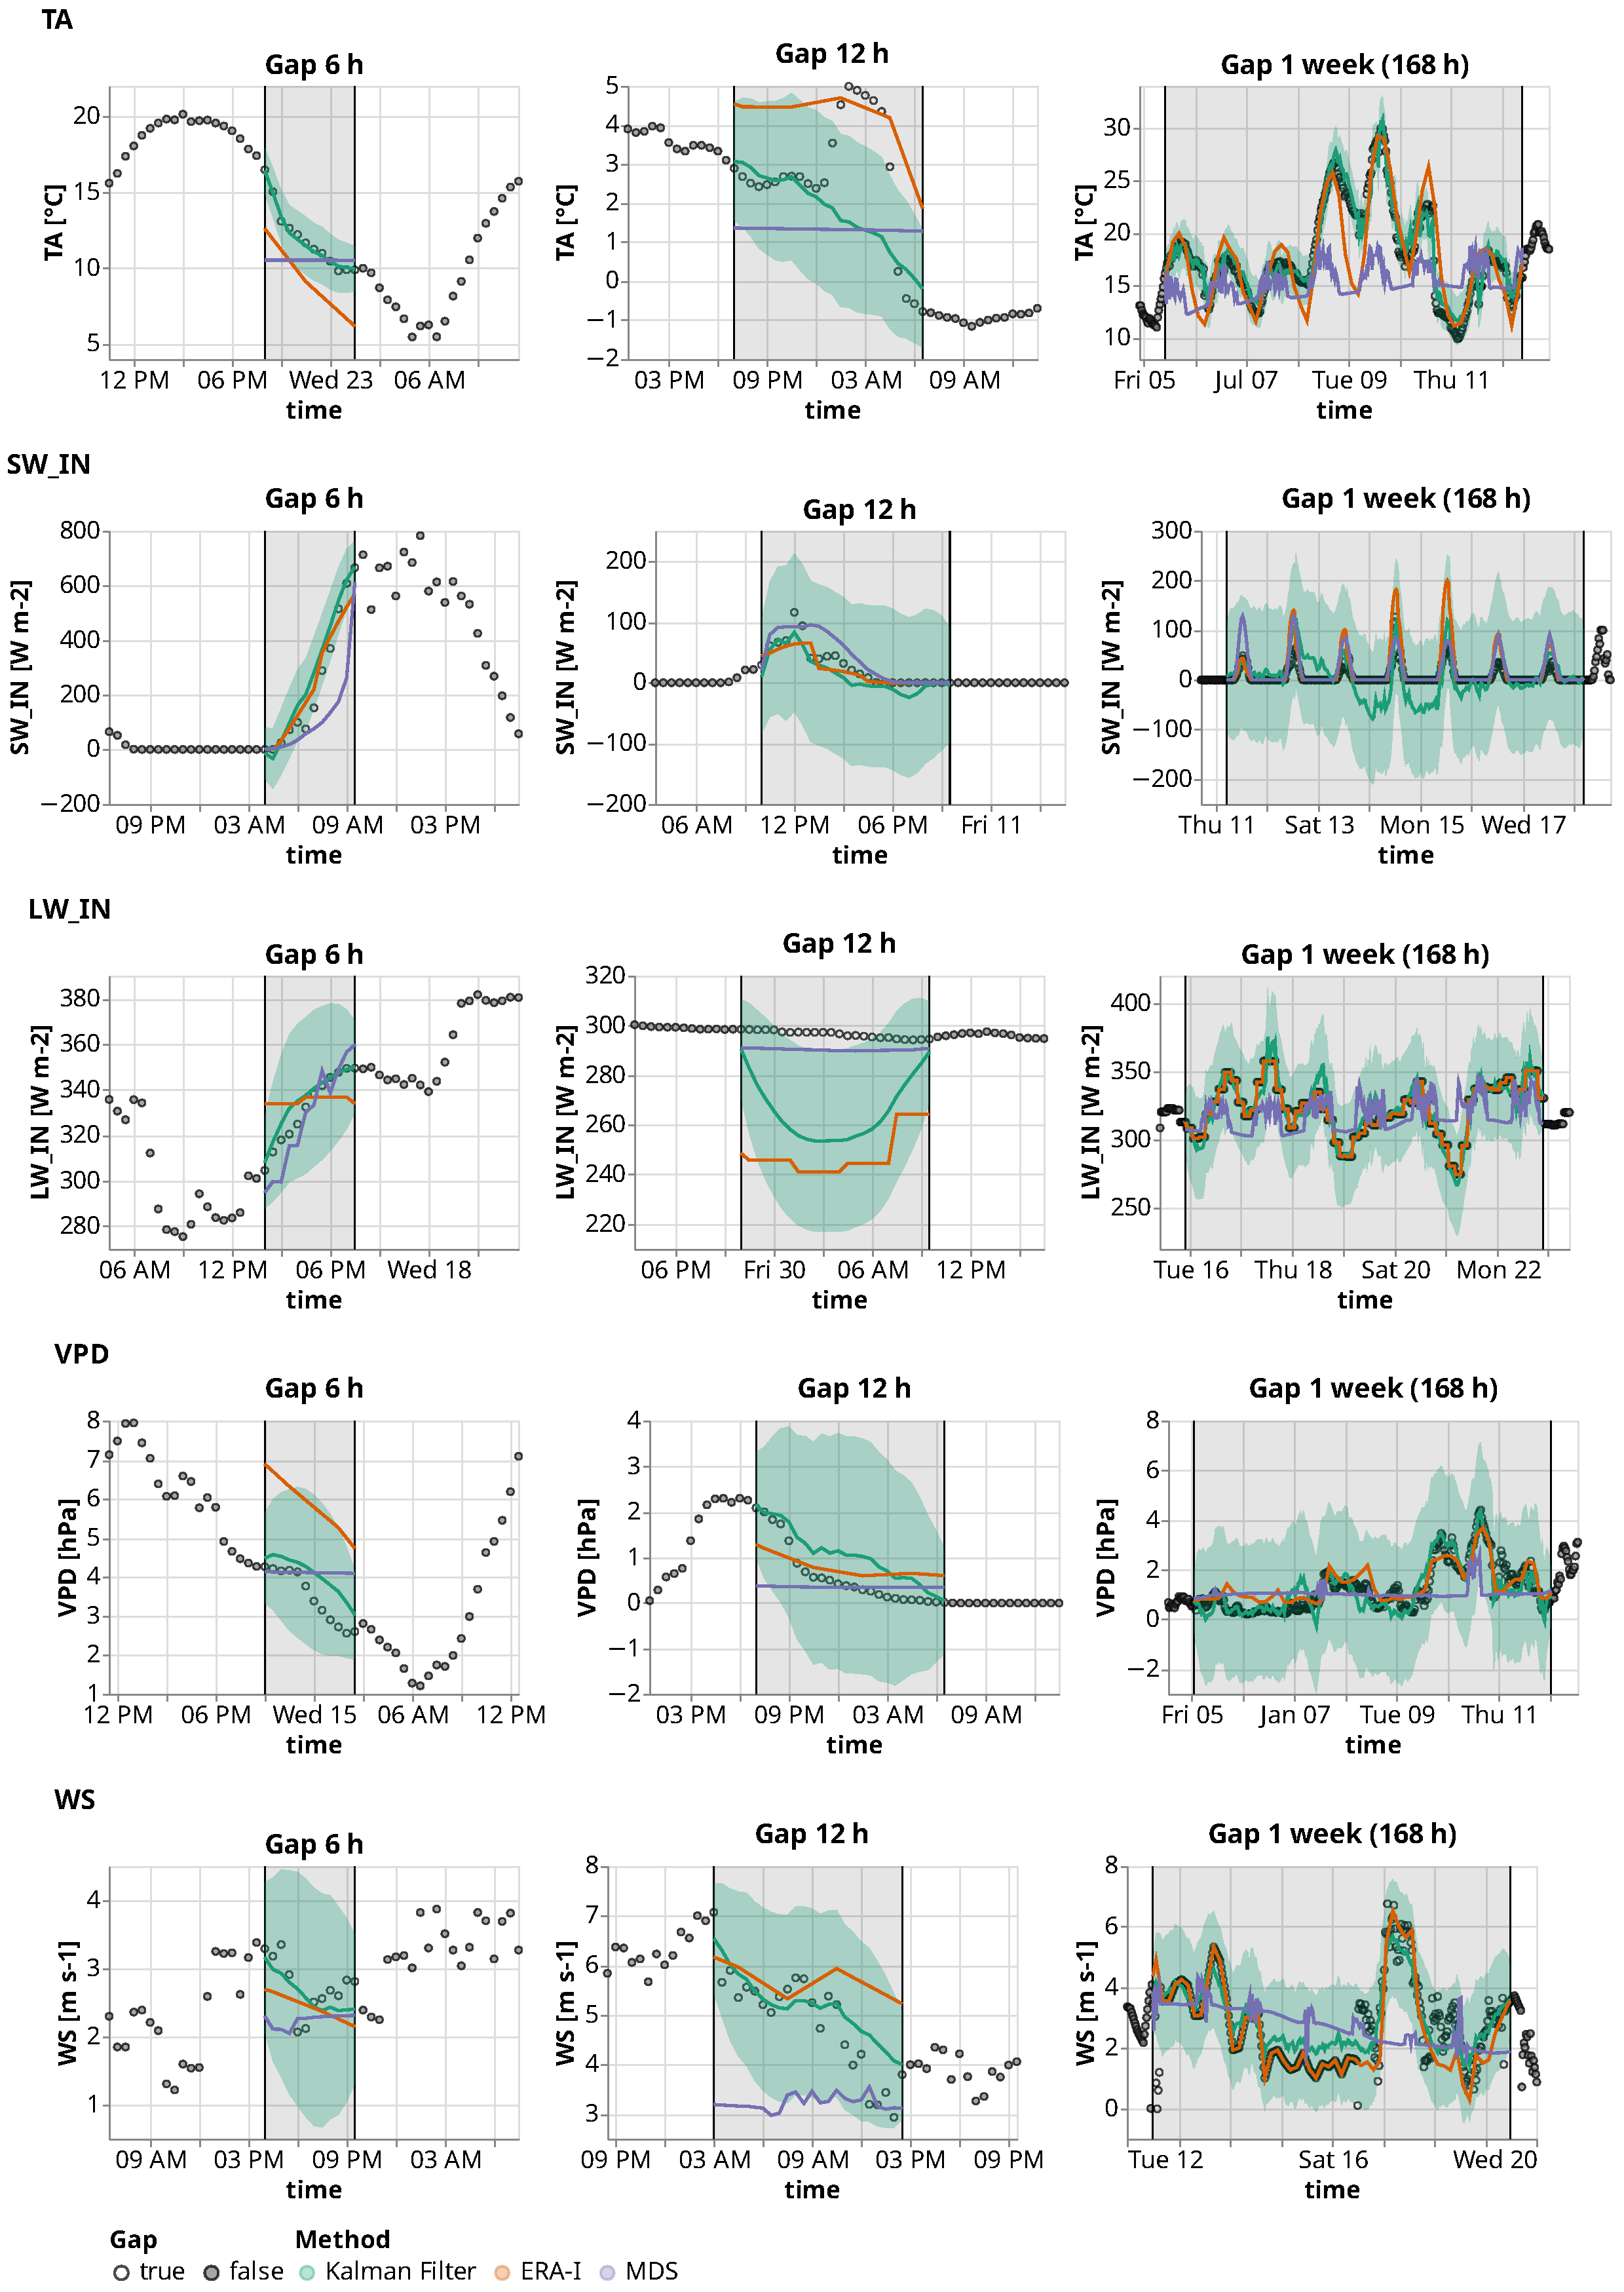
\includegraphics[width=5.7in]{timeseries_1_2}}
\caption{\CapTs{Third time series}{\texttt{TA}, \vv{SW\_IN}, \vv{LW\_IN}, \vv{VPD}, \vv{WS}}}
\label{fig:ts_3-1}
\end{figure}

\newgeometry{top=.7in}
\begin{figure}
\centerline{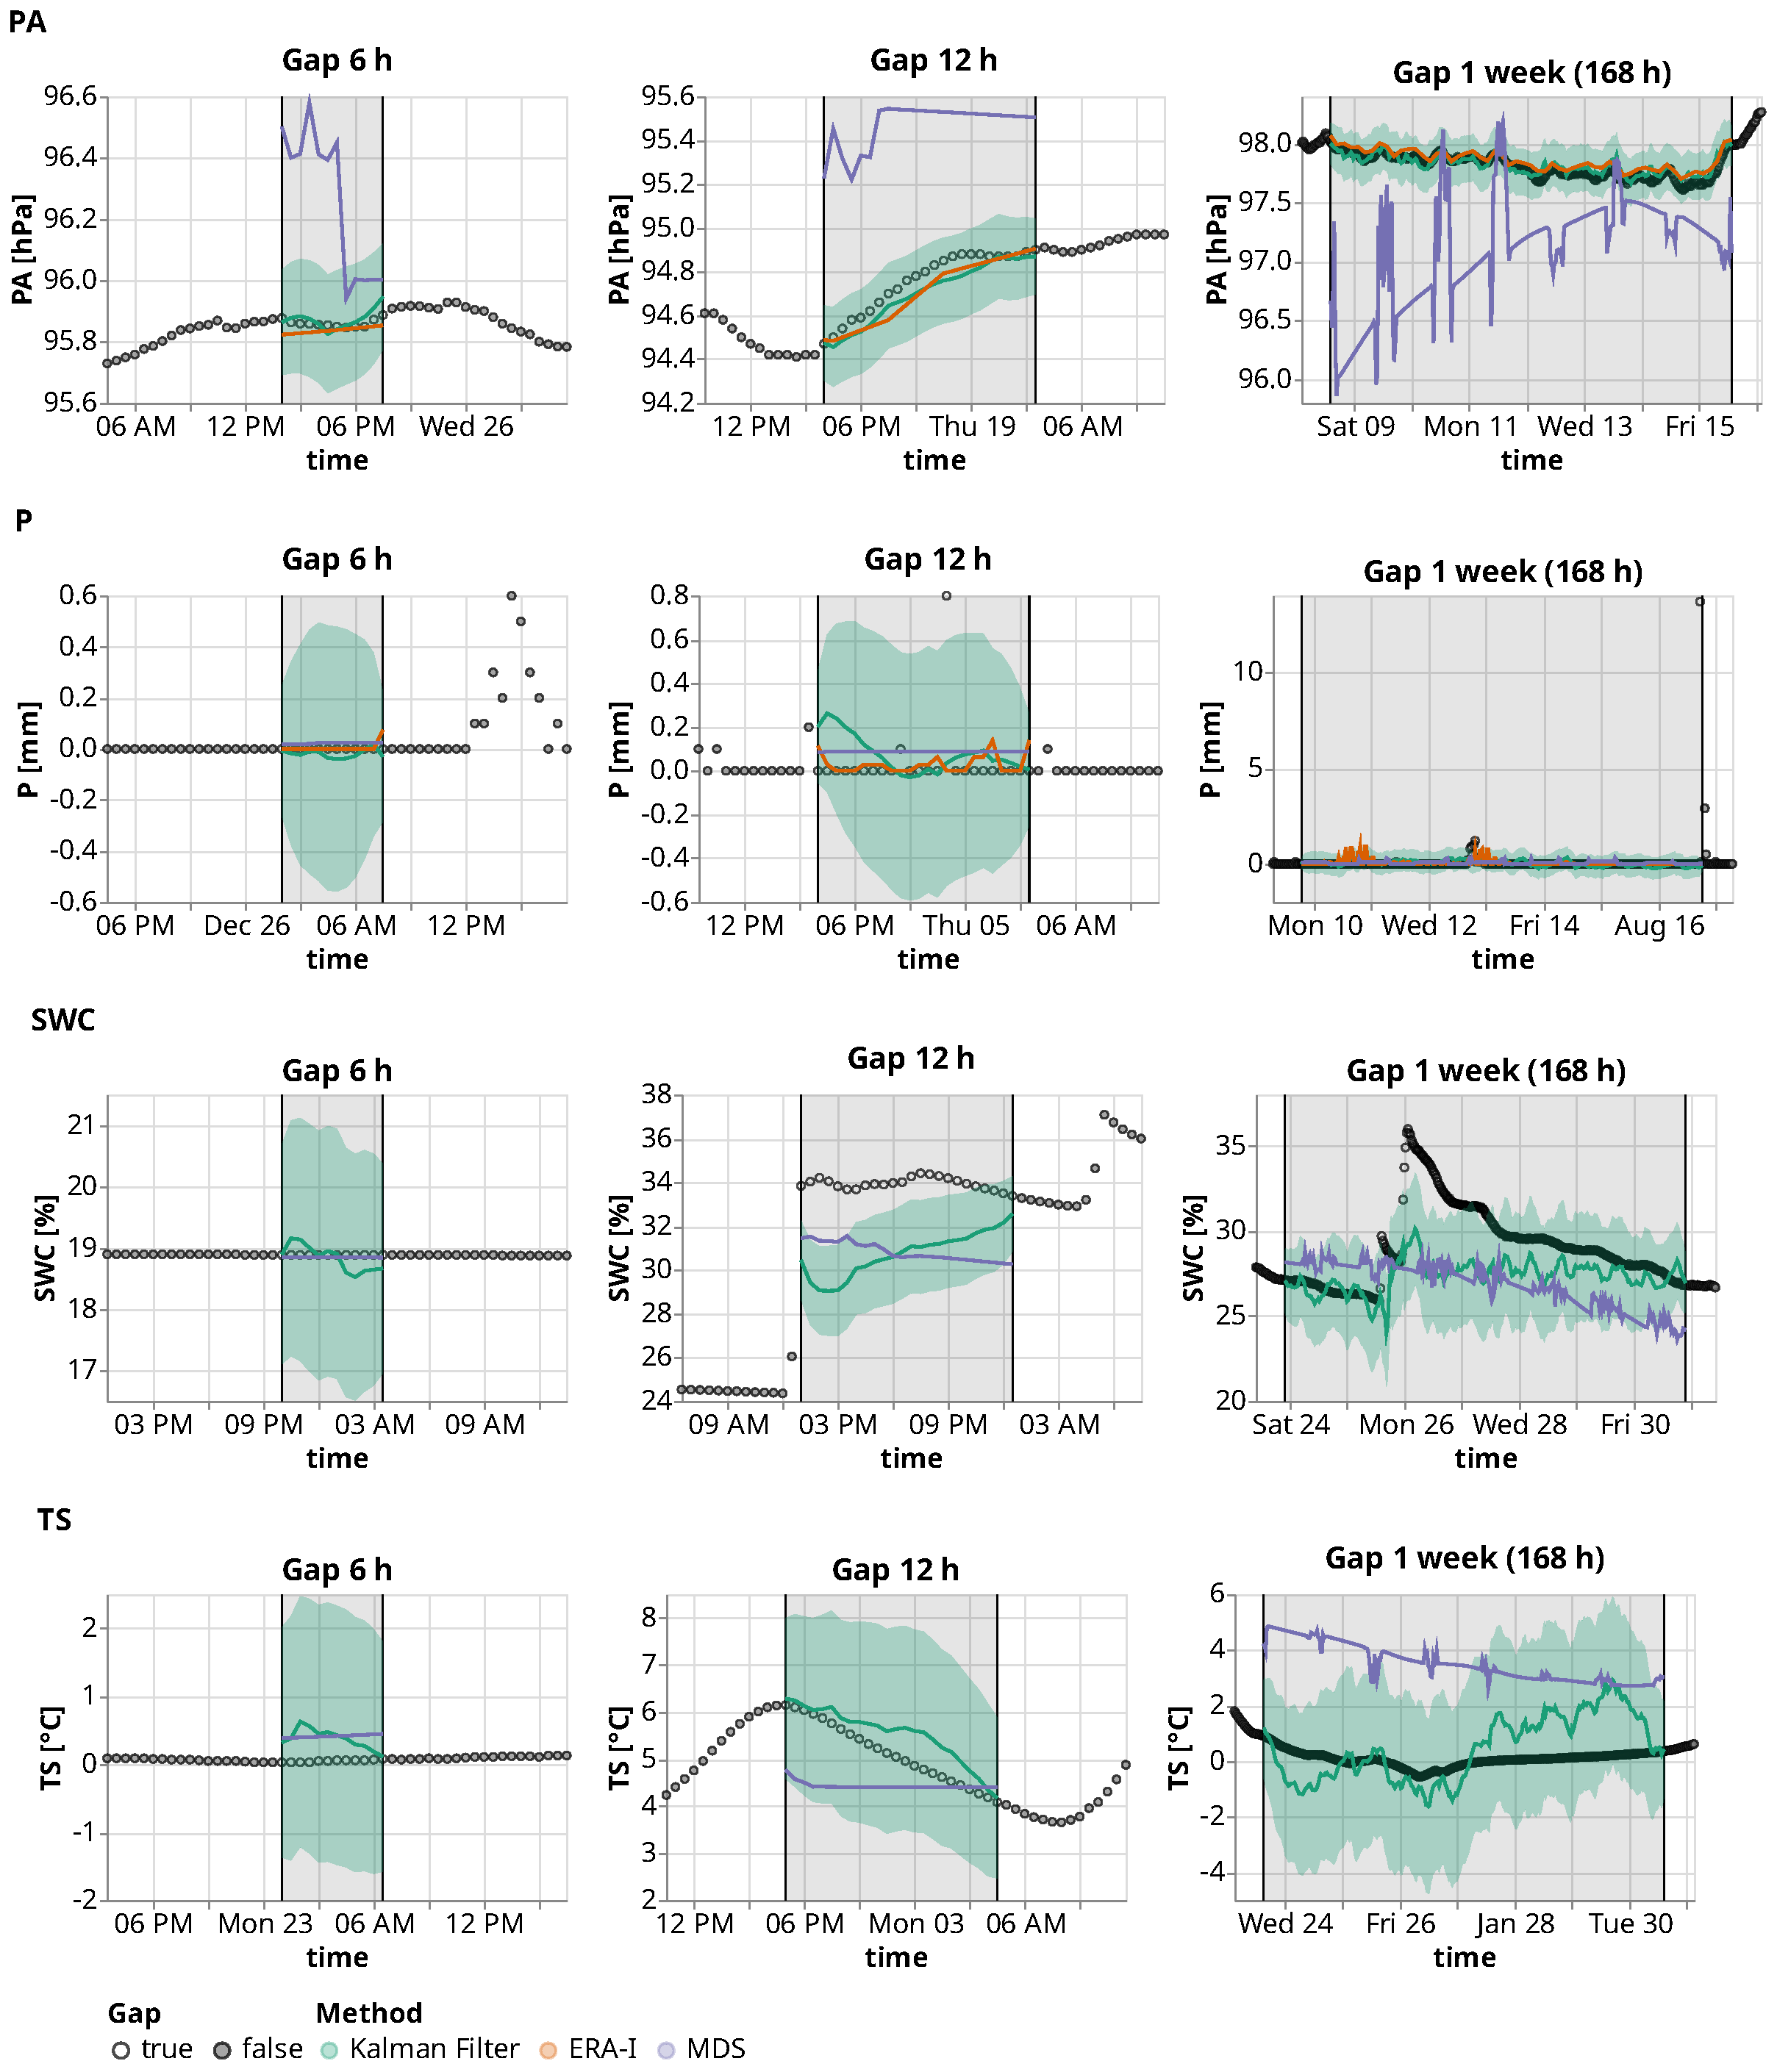
\includegraphics[width=\imgwidth]{timeseries_2_2}}
\caption{\CapTs{Third time series}{\texttt{PA}, \vv{P}, \vv{SWC}, \vv{TS}}}
\label{fig:ts_3-2}
\end{figure}
\restoregeometry

% \subsection{Additional Tables}

\newcommand{\CapGapLen}{Imputation performance of the KF in comparison to the state-of-the-art
methods: ERA-Interim (ERA-I) and Marginal Distribution Sampling (MDS), using mean and standard deviation of the \textit{Root Mean Square Error} (RMSE). The best method for each gap length is highlighted in bold. For each combination of gap length and variable, 500 artificial gaps were created.}
\include{tables/gap_len_fixed}

\newcommand{\CapControl}{Comparison of the KF performance between a model that uses control variables (\textit{KF-Gen-Sin-6\_336}) and models that do not use control variables (\textit{KF-Gen-Sin-6\_336-No\_Contr}). The table displays the mean, the standard deviation (std) and the standard error (se) of the \textit{Root Mean Square Error} (RMSE). In addition the difference (diff.) between the mean of two models is shown. The best method for each gap length is highlighted in bold. For each combination of gap length and variable, 500 artificial gaps were created.}
\begin{table}
\centering
\caption{RMSE Comparison Kalman filter with and without control variable. The best result for each for each gap length is highligthed in bold}
\label{control}
\begin{tabular}{p{2.1cm}c|rr|rr|r}
\toprule
 & type & \multicolumn{2}{r}{No Control} & \multicolumn{2}{r}{Control} &  \\
 & RMSE Standardized & mean & std & mean & std & diff. \\
Variable & Gap [$h$] &  &  &  &  &  \\
\midrule
\multirow[c]{4}{*}{\parbox{2.1cm}{\textbf{TA} [\si{°C}]}} & 6 & 0.114 & 0.071 & \bfseries 0.063 & 0.037 & 0.051 \\
 & 12 & 0.182 & 0.098 & \bfseries 0.097 & 0.074 & 0.085 \\
 & 24 & 0.259 & 0.163 & \bfseries 0.116 & 0.086 & 0.143 \\
 & 168 & 0.272 & 0.157 & \bfseries 0.139 & 0.086 & 0.132 \\
\cline{1-7}
\multirow[c]{4}{*}{\parbox{2.1cm}{\textbf{SW\_IN} [\si{W/m^2}]}} & 6 & 0.341 & 0.277 & \bfseries 0.238 & 0.237 & 0.103 \\
 & 12 & 0.549 & 0.330 & \bfseries 0.244 & 0.178 & 0.305 \\
 & 24 & 0.595 & 0.218 & \bfseries 0.283 & 0.136 & 0.312 \\
 & 168 & 0.636 & 0.212 & \bfseries 0.297 & 0.122 & 0.339 \\
\cline{1-7}
\multirow[c]{4}{*}{\parbox{2.1cm}{\textbf{LW\_IN} [\si{W/m^2}]}} & 6 & 0.344 & 0.210 & \bfseries 0.308 & 0.229 & 0.036 \\
 & 12 & 0.518 & 0.237 & \bfseries 0.385 & 0.227 & 0.133 \\
 & 24 & 0.543 & 0.226 & \bfseries 0.404 & 0.176 & 0.139 \\
 & 168 & 0.638 & 0.182 & \bfseries 0.431 & 0.179 & 0.207 \\
\cline{1-7}
\multirow[c]{4}{*}{\parbox{2.1cm}{\textbf{VPD} [\si{hPa}]}} & 6 & 0.178 & 0.162 & \bfseries 0.143 & 0.114 & 0.035 \\
 & 12 & 0.273 & 0.161 & \bfseries 0.196 & 0.126 & 0.078 \\
 & 24 & 0.375 & 0.228 & \bfseries 0.250 & 0.186 & 0.125 \\
 & 168 & 0.524 & 0.566 & \bfseries 0.287 & 0.153 & 0.237 \\
\cline{1-7}
\multirow[c]{4}{*}{\parbox{2.1cm}{\textbf{WS} [\si{m/s}]}} & 6 & 0.469 & 0.257 & \bfseries 0.339 & 0.198 & 0.130 \\
 & 12 & 0.661 & 0.404 & \bfseries 0.455 & 0.220 & 0.205 \\
 & 24 & 0.782 & 0.363 & \bfseries 0.463 & 0.173 & 0.319 \\
 & 168 & 0.898 & 0.334 & \bfseries 0.586 & 0.209 & 0.312 \\
\cline{1-7}
\multirow[c]{4}{*}{\parbox{2.1cm}{\textbf{PA} [\si{hPa}]}} & 6 & 0.154 & 0.103 & \bfseries 0.057 & 0.031 & 0.097 \\
 & 12 & 0.357 & 0.228 & \bfseries 0.062 & 0.029 & 0.295 \\
 & 24 & 0.578 & 0.336 & \bfseries 0.067 & 0.033 & 0.511 \\
 & 168 & 0.959 & 0.417 & \bfseries 0.088 & 0.058 & 0.872 \\
\cline{1-7}
\multirow[c]{4}{*}{\parbox{2.1cm}{\textbf{P} [\si{mm}]}} & 6 & \bfseries 0.376 & 0.964 & 0.462 & 0.768 & 0.085 \\
 & 12 & 0.671 & 1.054 & \bfseries 0.426 & 0.549 & 0.246 \\
 & 24 & \bfseries 0.468 & 0.538 & 0.702 & 1.202 & 0.234 \\
 & 168 & \bfseries 0.720 & 0.578 & 0.782 & 0.695 & 0.063 \\
\cline{1-7}
\multirow[c]{4}{*}{\parbox{2.1cm}{\textbf{SWC} [\si{\%}]}} & 6 & 0.120 & 0.081 & \bfseries 0.054 & 0.038 & 0.066 \\
 & 12 & 0.281 & 0.169 & \bfseries 0.059 & 0.034 & 0.223 \\
 & 24 & 0.513 & 0.335 & \bfseries 0.071 & 0.046 & 0.443 \\
 & 168 & 0.774 & 0.319 & \bfseries 0.149 & 0.075 & 0.625 \\
\cline{1-7}
\multirow[c]{4}{*}{\parbox{2.1cm}{\textbf{TS} [\si{°C}]}} & 6 & 0.132 & 0.102 & \bfseries 0.066 & 0.073 & 0.066 \\
 & 12 & 0.201 & 0.131 & \bfseries 0.091 & 0.053 & 0.110 \\
 & 24 & 0.281 & 0.169 & \bfseries 0.170 & 0.149 & 0.111 \\
 & 168 & 0.356 & 0.196 & \bfseries 0.290 & 0.188 & 0.065 \\
\cline{1-7}
\bottomrule
\end{tabular}
\end{table}


\newcommand{\CapGapSingle}{Comparison of the KF performance of a gap when only one variable missing and all other variables are missing. The model used for imputation is always \textit{KF-Gen-Multi-6\_336}. The table displays the mean, the standard deviation (std) and the standard error (se) of the \textit{Root Mean Square Error} (RMSE). In addition the difference (diff.) between the mean of two models is shown. The best method for each gap length is highlighted in bold. For each combination of gap length and variable, 500 artificial gaps were created.}
\begin{table}
\centering
\begin{tabular}{p{2.1cm}c|rr|rr|r}
\toprule
 & Gap & \multicolumn{2}{r}{Only one var} & \multicolumn{2}{r}{All variables} &  \\
 & RMSE Standardized & mean & std & mean & std & diff. \\
Variable & Gap [$h$] &  &  &  &  &  \\
\midrule
\multirow[c]{4}{*}{\parbox{2.1cm}{\textbf{TA} [\si{°C}]}} & 3 & 0.048 & 0.026 & \bfseries 0.047 & 0.032 & 0.001 \\
 & 6 & \bfseries 0.067 & 0.037 & 0.080 & 0.054 & 0.013 \\
 & 12 & \bfseries 0.090 & 0.048 & 0.115 & 0.071 & 0.024 \\
 & 15 & \bfseries 0.098 & 0.057 & 0.130 & 0.082 & 0.033 \\
\cline{1-7}
\multirow[c]{4}{*}{\parbox{2.1cm}{\textbf{SW\_IN} [\si{W/m^2}]}} & 3 & \bfseries 0.205 & 0.230 & 0.229 & 0.296 & 0.024 \\
 & 6 & \bfseries 0.236 & 0.215 & 0.282 & 0.314 & 0.047 \\
 & 12 & 0.259 & 0.197 & \bfseries 0.259 & 0.250 & 0.000 \\
 & 15 & 0.259 & 0.180 & \bfseries 0.237 & 0.191 & 0.022 \\
\cline{1-7}
\multirow[c]{4}{*}{\parbox{2.1cm}{\textbf{LW\_IN} [\si{W/m^2}]}} & 3 & \bfseries 0.201 & 0.197 & 0.214 & 0.195 & 0.013 \\
 & 6 & \bfseries 0.259 & 0.202 & 0.283 & 0.187 & 0.025 \\
 & 12 & 0.356 & 0.225 & \bfseries 0.353 & 0.220 & 0.003 \\
 & 15 & 0.365 & 0.232 & \bfseries 0.360 & 0.218 & 0.005 \\
\cline{1-7}
\multirow[c]{4}{*}{\parbox{2.1cm}{\textbf{VPD} [\si{hPa}]}} & 3 & \bfseries 0.103 & 0.086 & 0.122 & 0.123 & 0.019 \\
 & 6 & \bfseries 0.138 & 0.123 & 0.178 & 0.156 & 0.041 \\
 & 12 & \bfseries 0.175 & 0.117 & 0.220 & 0.167 & 0.045 \\
 & 15 & \bfseries 0.206 & 0.132 & 0.256 & 0.207 & 0.050 \\
\cline{1-7}
\multirow[c]{4}{*}{\parbox{2.1cm}{\textbf{WS} [\si{m/s}]}} & 3 & \bfseries 0.291 & 0.178 & 0.317 & 0.160 & 0.026 \\
 & 6 & \bfseries 0.372 & 0.186 & 0.386 & 0.253 & 0.014 \\
 & 12 & \bfseries 0.430 & 0.241 & 0.464 & 0.220 & 0.034 \\
 & 15 & \bfseries 0.453 & 0.208 & 0.499 & 0.258 & 0.046 \\
\cline{1-7}
\multirow[c]{4}{*}{\parbox{2.1cm}{\textbf{PA} [\si{hPa}]}} & 3 & 0.040 & 0.024 & \bfseries 0.034 & 0.023 & 0.006 \\
 & 6 & 0.051 & 0.034 & \bfseries 0.048 & 0.032 & 0.003 \\
 & 12 & \bfseries 0.064 & 0.047 & 0.065 & 0.051 & 0.001 \\
 & 15 & 0.063 & 0.030 & \bfseries 0.062 & 0.040 & 0.002 \\
\cline{1-7}
\multirow[c]{4}{*}{\parbox{2.1cm}{\textbf{P} [\si{mm}]}} & 3 & 0.369 & 0.803 & \bfseries 0.296 & 0.408 & 0.073 \\
 & 6 & 0.624 & 1.487 & \bfseries 0.379 & 0.964 & 0.245 \\
 & 12 & \bfseries 0.456 & 0.759 & 0.517 & 1.119 & 0.061 \\
 & 15 & 0.566 & 1.222 & \bfseries 0.431 & 0.675 & 0.135 \\
\cline{1-7}
\multirow[c]{4}{*}{\parbox{2.1cm}{\textbf{SWC} [\si{\%}]}} & 3 & 0.044 & 0.034 & \bfseries 0.020 & 0.032 & 0.024 \\
 & 6 & 0.055 & 0.049 & \bfseries 0.027 & 0.038 & 0.028 \\
 & 12 & 0.066 & 0.053 & \bfseries 0.034 & 0.042 & 0.032 \\
 & 15 & 0.071 & 0.055 & \bfseries 0.038 & 0.048 & 0.033 \\
\cline{1-7}
\multirow[c]{4}{*}{\parbox{2.1cm}{\textbf{TS} [\si{°C}]}} & 3 & 0.048 & 0.030 & \bfseries 0.033 & 0.031 & 0.015 \\
 & 6 & 0.068 & 0.051 & \bfseries 0.055 & 0.047 & 0.013 \\
 & 12 & \bfseries 0.099 & 0.073 & 0.100 & 0.125 & 0.001 \\
 & 15 & 0.121 & 0.113 & \bfseries 0.118 & 0.131 & 0.003 \\
\cline{1-7}
\bottomrule
\end{tabular}
\end{table}



\newcommand{\CapGeneric}{Comparison between KF models fine-tuned to each variable ( \textit{KF-\textlangle var\textrangle-Sin-6\_336}) and generic model trained for gaps in any variable (\textit{KF-Gen-Sin-6\_336}). The table displays the mean, the standard deviation (std) and the standard error (se) of the \textit{Root Mean Square Error} (RMSE). In addition the difference (diff.) between the mean of two models is shown. The best method for each gap length is highlighted in bold. For each combination of gap length and variable, 500 artificial gaps were created.}
\begin{table}
\centering
\caption{\CapGeneric}
\label{generic}
\begin{tabular}{p{2.1cm}c|rr|rr|r}
\toprule
 & type & \multicolumn{2}{r}{Generic} & \multicolumn{2}{r}{Finetuned one var} &  \\
 & RMSE Standardized & mean & std & mean & std & diff. \\
Variable & Gap [$h$] &  &  &  &  &  \\
\midrule
\multirow[c]{4}{*}{\parbox{2.1cm}{\textbf{TA}}} & 6 & 0.092 & 0.056 & \bfseries 0.055 & 0.033 & -0.037 \\
 & 12 & 0.118 & 0.074 & \bfseries 0.077 & 0.052 & -0.041 \\
 & 24 & 0.147 & 0.077 & \bfseries 0.101 & 0.059 & -0.046 \\
 & 168 & 0.174 & 0.064 & \bfseries 0.129 & 0.048 & -0.045 \\
\cline{1-7}
\multirow[c]{4}{*}{\parbox{2.1cm}{\textbf{SW\_IN}}} & 6 & 0.256 & 0.165 & \bfseries 0.209 & 0.167 & -0.047 \\
 & 12 & 0.315 & 0.165 & \bfseries 0.258 & 0.164 & -0.057 \\
 & 24 & 0.339 & 0.129 & \bfseries 0.281 & 0.132 & -0.059 \\
 & 168 & 0.358 & 0.103 & \bfseries 0.298 & 0.119 & -0.060 \\
\cline{1-7}
\multirow[c]{4}{*}{\parbox{2.1cm}{\textbf{LW\_IN}}} & 6 & 0.299 & 0.201 & \bfseries 0.257 & 0.200 & -0.043 \\
 & 12 & 0.368 & 0.197 & \bfseries 0.326 & 0.209 & -0.041 \\
 & 24 & 0.400 & 0.176 & \bfseries 0.359 & 0.186 & -0.042 \\
 & 168 & 0.466 & 0.141 & \bfseries 0.406 & 0.165 & -0.060 \\
\cline{1-7}
\multirow[c]{4}{*}{\parbox{2.1cm}{\textbf{VPD}}} & 6 & 0.138 & 0.105 & \bfseries 0.097 & 0.089 & -0.041 \\
 & 12 & 0.227 & 0.184 & \bfseries 0.169 & 0.165 & -0.058 \\
 & 24 & 0.273 & 0.207 & \bfseries 0.202 & 0.160 & -0.070 \\
 & 168 & 0.325 & 0.154 & \bfseries 0.264 & 0.153 & -0.061 \\
\cline{1-7}
\multirow[c]{4}{*}{\parbox{2.1cm}{\textbf{WS}}} & 6 & 0.572 & 0.523 & \bfseries 0.365 & 0.201 & -0.206 \\
 & 12 & 0.660 & 0.409 & \bfseries 0.482 & 0.265 & -0.178 \\
 & 24 & 0.676 & 0.374 & \bfseries 0.511 & 0.270 & -0.166 \\
 & 168 & 0.782 & 0.265 & \bfseries 0.569 & 0.190 & -0.212 \\
\cline{1-7}
\multirow[c]{4}{*}{\parbox{2.1cm}{\textbf{PA}}} & 6 & 0.099 & 0.066 & \bfseries 0.054 & 0.032 & -0.045 \\
 & 12 & 0.116 & 0.061 & \bfseries 0.060 & 0.031 & -0.056 \\
 & 24 & 0.137 & 0.076 & \bfseries 0.072 & 0.069 & -0.065 \\
 & 168 & 0.159 & 0.068 & \bfseries 0.081 & 0.054 & -0.078 \\
\cline{1-7}
\multirow[c]{4}{*}{\parbox{2.1cm}{\textbf{P}}} & 6 & \bfseries 0.542 & 0.991 & \bfseries 0.542 & 0.991 & 0.000 \\
 & 12 & \bfseries 0.627 & 1.035 & \bfseries 0.627 & 1.035 & 0.000 \\
 & 24 & \bfseries 0.628 & 0.575 & \bfseries 0.628 & 0.575 & 0.000 \\
 & 168 & \bfseries 0.881 & 0.573 & \bfseries 0.881 & 0.573 & 0.000 \\
\cline{1-7}
\multirow[c]{4}{*}{\parbox{2.1cm}{\textbf{SWC}}} & 6 & 0.152 & 0.107 & \bfseries 0.051 & 0.034 & -0.102 \\
 & 12 & 0.245 & 0.154 & \bfseries 0.067 & 0.043 & -0.177 \\
 & 24 & 0.393 & 0.223 & \bfseries 0.079 & 0.053 & -0.314 \\
 & 168 & 0.719 & 0.314 & \bfseries 0.169 & 0.104 & -0.550 \\
\cline{1-7}
\multirow[c]{4}{*}{\parbox{2.1cm}{\textbf{TS}}} & 6 & 0.168 & 0.115 & \bfseries 0.065 & 0.068 & -0.103 \\
 & 12 & 0.226 & 0.135 & \bfseries 0.088 & 0.087 & -0.138 \\
 & 24 & 0.286 & 0.152 & \bfseries 0.129 & 0.128 & -0.157 \\
 & 168 & 0.362 & 0.176 & \bfseries 0.317 & 0.218 & -0.046 \\
\cline{1-7}
\bottomrule
\end{tabular}
\end{table}


\newgeometry{top=.7in}
\newcommand{\CapTrain}{ The table displays the KF training difficulties. For a gap in one variable, three models are compared: a model trained with gaps in multiple variables (``Multi vars'', \textit{KF-Gen-Multi-6\_336}), a model trained with gaps of only one variable (``Only one var'', \textit{KF-Gen-Sin-6\_336}) and one model trained with gaps in multiple variables but initialized with random parameters (``Random params'', \textit{KF-Gen-Multi-6\_336-Rand}). The models are expected to have comparable performances. The table displays the mean, the standard deviation (std) of the \textit{Root Mean Square Error} (RMSE). The best method for each gap length is highlighted in bold. For each combination of gap length and variable, 500 artificial gaps were created.}
\begin{table}
\centering
\caption{\CapTrain}
\label{tbl:train_compare}
\begin{tabular}{p{2.1cm}l|rr|rr|rr}
\toprule
 & Train & \multicolumn{2}{r}{Multi vars} & \multicolumn{2}{r}{Only one var} & \multicolumn{2}{r}{Random params} \\
 & Stand. RMSE & mean & std & mean & std & mean & std \\
Variable & Gap [$h$] &  &  &  &  &  &  \\
\midrule
\multirow[c]{4}{*}{\textbf{TA}} & 3 h & \bfseries 0.029 & 0.024 & 0.066 & 0.050 & 0.060 & 0.045 \\
 & 6 h & \bfseries 0.044 & 0.033 & 0.093 & 0.062 & 0.080 & 0.055 \\
 & 12 h & \bfseries 0.073 & 0.050 & 0.133 & 0.092 & 0.117 & 0.085 \\
 & 15 h & \bfseries 0.077 & 0.051 & 0.131 & 0.072 & 0.111 & 0.068 \\
\cline{1-8}
\multirow[c]{4}{*}{\textbf{SW\_IN}} & 3 h & \bfseries 0.178 & 0.176 & 0.202 & 0.178 & 0.259 & 0.220 \\
 & 6 h & \bfseries 0.210 & 0.170 & 0.249 & 0.176 & 0.283 & 0.209 \\
 & 12 h & \bfseries 0.269 & 0.172 & 0.308 & 0.167 & 0.333 & 0.193 \\
 & 15 h & \bfseries 0.270 & 0.166 & 0.315 & 0.164 & 0.334 & 0.188 \\
\cline{1-8}
\multirow[c]{4}{*}{\textbf{LW\_IN}} & 3 h & \bfseries 0.200 & 0.169 & 0.215 & 0.177 & 0.298 & 0.203 \\
 & 6 h & \bfseries 0.270 & 0.216 & 0.297 & 0.229 & 0.342 & 0.229 \\
 & 12 h & \bfseries 0.332 & 0.224 & 0.377 & 0.241 & 0.398 & 0.259 \\
 & 15 h & \bfseries 0.357 & 0.208 & 0.390 & 0.208 & 0.398 & 0.225 \\
\cline{1-8}
\multirow[c]{4}{*}{\textbf{VPD}} & 3 h & \bfseries 0.064 & 0.060 & 0.097 & 0.079 & 0.150 & 0.128 \\
 & 6 h & \bfseries 0.098 & 0.096 & 0.148 & 0.113 & 0.193 & 0.174 \\
 & 12 h & \bfseries 0.168 & 0.156 & 0.223 & 0.161 & 0.240 & 0.192 \\
 & 15 h & \bfseries 0.186 & 0.159 & 0.241 & 0.168 & 0.254 & 0.210 \\
\cline{1-8}
\multirow[c]{4}{*}{\textbf{WS}} & 3 h & \bfseries 0.305 & 0.183 & 0.471 & 0.460 & 0.447 & 0.300 \\
 & 6 h & \bfseries 0.372 & 0.210 & 0.576 & 0.466 & 0.482 & 0.309 \\
 & 12 h & \bfseries 0.429 & 0.195 & 0.649 & 0.481 & 0.523 & 0.270 \\
 & 15 h & \bfseries 0.479 & 0.230 & 0.691 & 0.457 & 0.540 & 0.293 \\
\cline{1-8}
\multirow[c]{4}{*}{\textbf{PA}} & 3 h & \bfseries 0.025 & 0.019 & 0.073 & 0.062 & 0.067 & 0.057 \\
 & 6 h & \bfseries 0.035 & 0.021 & 0.095 & 0.061 & 0.098 & 0.077 \\
 & 12 h & \bfseries 0.051 & 0.045 & 0.117 & 0.073 & 0.118 & 0.089 \\
 & 15 h & \bfseries 0.059 & 0.040 & 0.128 & 0.080 & 0.115 & 0.076 \\
\cline{1-8}
\multirow[c]{4}{*}{\textbf{P}} & 3 h & \bfseries 0.348 & 0.680 & 0.411 & 1.510 & 0.371 & 0.713 \\
 & 6 h & \bfseries 0.400 & 0.618 & 0.487 & 0.718 & 0.425 & 0.704 \\
 & 12 h & \bfseries 0.511 & 0.851 & 0.706 & 1.150 & 0.535 & 0.981 \\
 & 15 h & \bfseries 0.453 & 0.598 & 0.618 & 0.756 & 0.470 & 0.698 \\
\cline{1-8}
\multirow[c]{4}{*}{\textbf{SWC}} & 3 h & \bfseries 0.012 & 0.029 & 0.095 & 0.076 & 0.106 & 0.075 \\
 & 6 h & \bfseries 0.018 & 0.031 & 0.151 & 0.108 & 0.153 & 0.107 \\
 & 12 h & \bfseries 0.027 & 0.037 & 0.245 & 0.160 & 0.246 & 0.215 \\
 & 15 h & \bfseries 0.033 & 0.041 & 0.282 & 0.228 & 0.278 & 0.208 \\
\cline{1-8}
\multirow[c]{4}{*}{\textbf{TS}} & 3 h & \bfseries 0.024 & 0.018 & 0.102 & 0.082 & 0.047 & 0.037 \\
 & 6 h & \bfseries 0.048 & 0.048 & 0.164 & 0.106 & 0.076 & 0.074 \\
 & 12 h & \bfseries 0.083 & 0.086 & 0.231 & 0.158 & 0.122 & 0.134 \\
 & 15 h & \bfseries 0.117 & 0.129 & 0.271 & 0.191 & 0.154 & 0.161 \\
\cline{1-8}
\bottomrule
\end{tabular}
\end{table}

\restoregeometry

\newcommand{\CapStd}{Standard deviation of the meteorological variables for the entire Hainich FLUXNET 2015 dataset ($\sigma_Y$).}
\begin{table}
\centering
\caption{\CapStd}
\label{tbl:hai_std}
\begin{tabular}{lrl}
\toprule
Variable & std & unit \\
\midrule
TA & 7.925 & \si{°C} \\
SW\_IN & 204.003 & \si{W/m^2} \\
LW\_IN & 41.956 & \si{hPa} \\
VPD & 4.368 & \si{hPa} \\
WS & 1.625 & \si{mm} \\
PA & 0.855 & \si{m/s} \\
P & 0.280 & \si{W/m^2} \\
SWC & 8.913 & \si{\%} \\
TS & 5.659 & \si{°C} \\
\bottomrule
\end{tabular}
\end{table}


% \subsection{Gap length distribution in FLUXNET}

\begin{figure}[H]
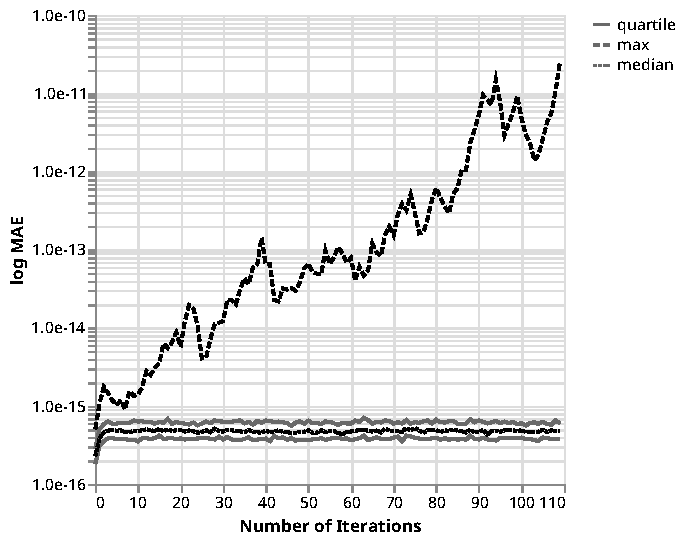
\includegraphics[width=\textwidth]{numerical_stability}
 \caption{Numerical stability comparison between Standard KF implementation and Square Root KF. For 100 times, the filters were initialized with a local trend model (drawn from a uniform distribution range 0-1) and then 110 observations processed using both models. At each time step, the Mean Absolute Error (MAE) was calculated between the state covariance from the Standard KF and the Square Root KF. The plot shows the median (black dotted line), 1st and 3rd quartile (gray lines) and the maximum of the MAE across the 100 samples (black dashed line).}
 \label{fig:num_stab}
\end{figure}

\begin{figure}
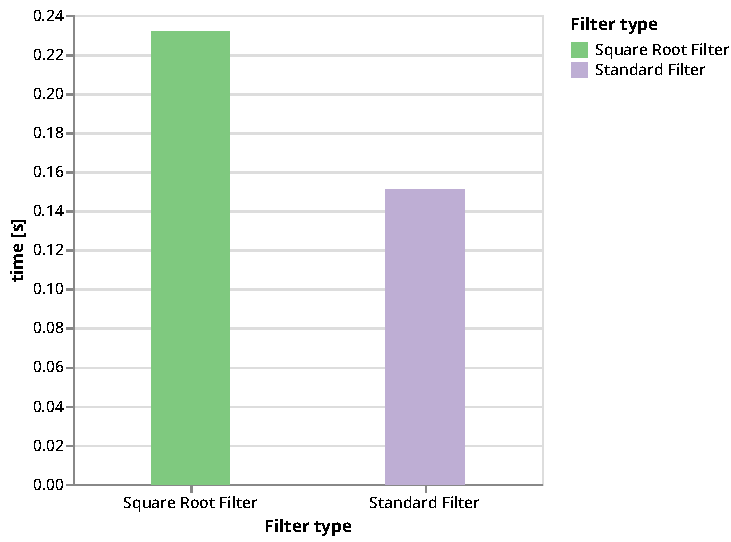
\includegraphics[width=\textwidth]{perf_sr}
 \caption{Performance comparison between Standard KF and Square Root KF. The bar height shows the mean execution time for 100 samples with the following settings: number of observations: 100, dimension observations: 9, dimension state: 18, dimension control: 14, batch size: 20. The models were initialized with local trend parameters. The data was randomly generated by sampling a uniform distribution between 0 and 1, without any missing data.}
 \label{fig:num_stab_perf}
\end{figure}

% The entire FLUXNET 2015 dataset was used to compute the distribution of gap lengths across the all the sites for each variable. A gap was definite when the QC flag of the variable is different from 0 or the data itself is missing. Figure \ref{fig:gap_len_dist} shows the complete distribution of the gaps, while Figure \ref{fig:gap_len_dist_small} focuses only on gaps shorter than a week.


\begin{figure}
\centerline{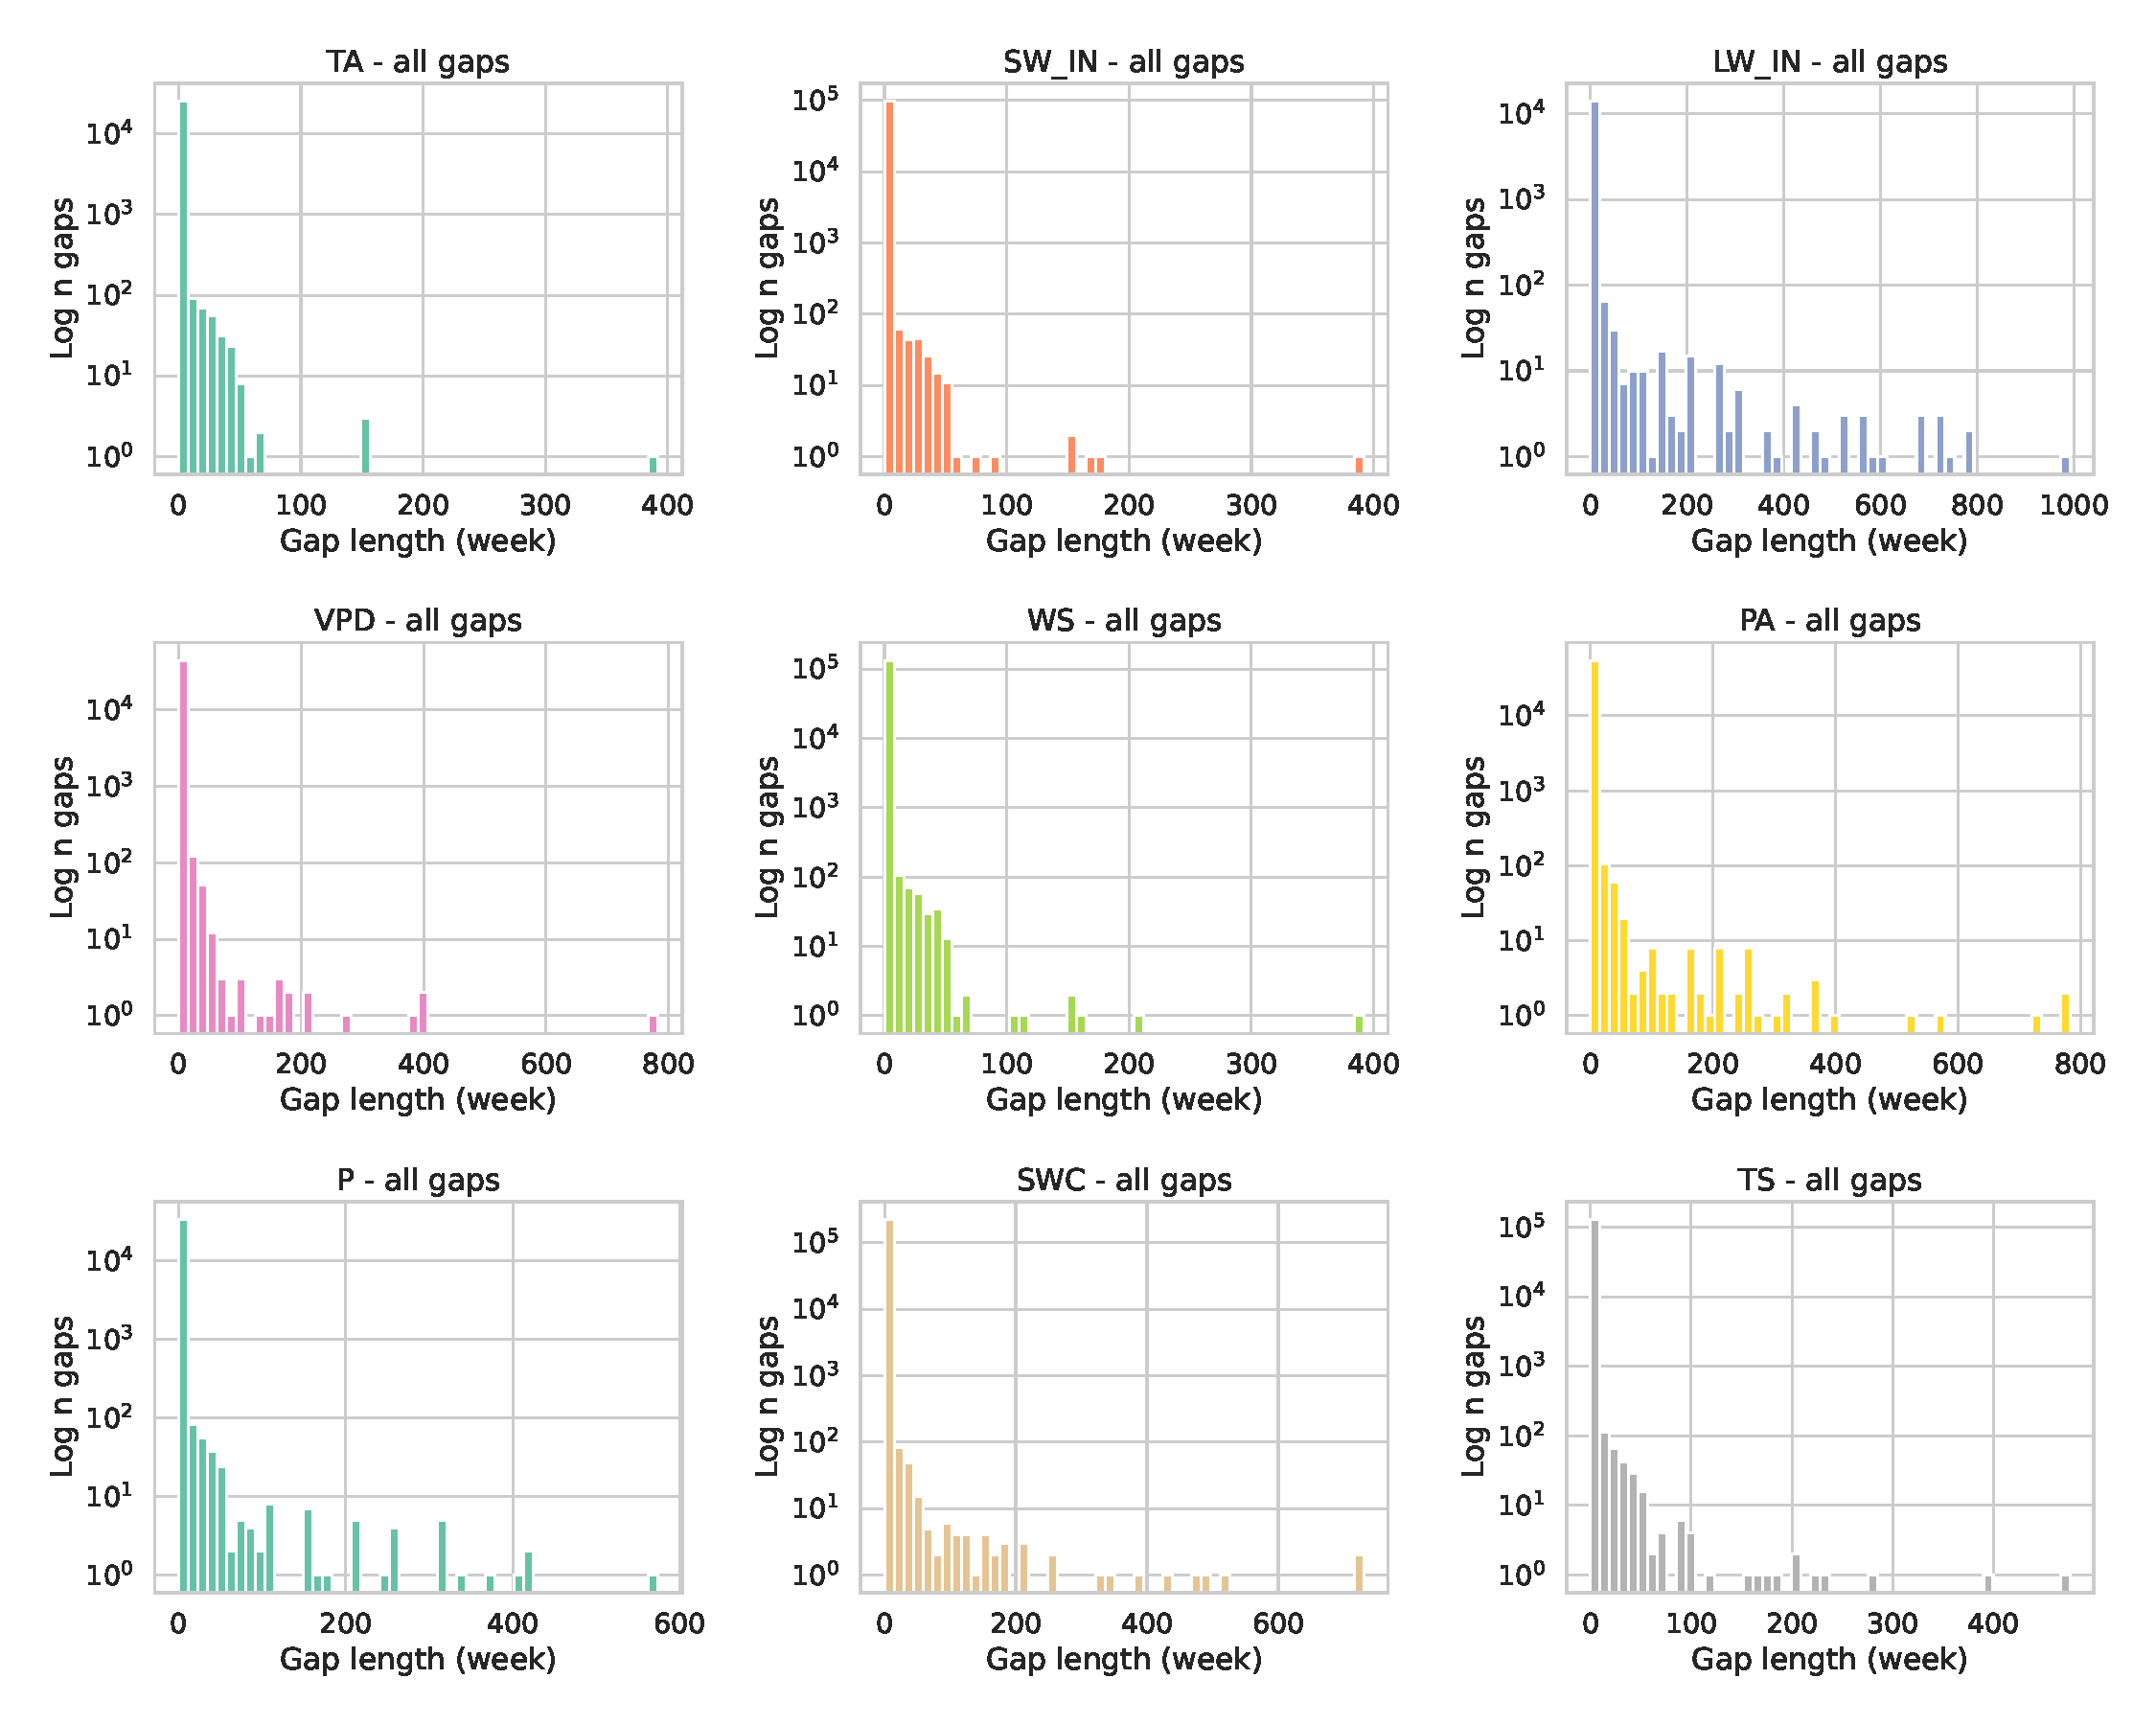
\includegraphics[width=\imgwidth]{gap_len_dist}}
\caption{Distribution of the gap lengths for all sites in the FLUXNET 2015 dataset for meteorological variables. The y axis displays the logarithm of the number of gaps. The length of the gap is the number of records where the QC flag is different than 0.}
\label{fig:gap_len_dist}
\end{figure}
\begin{figure}
\centerline{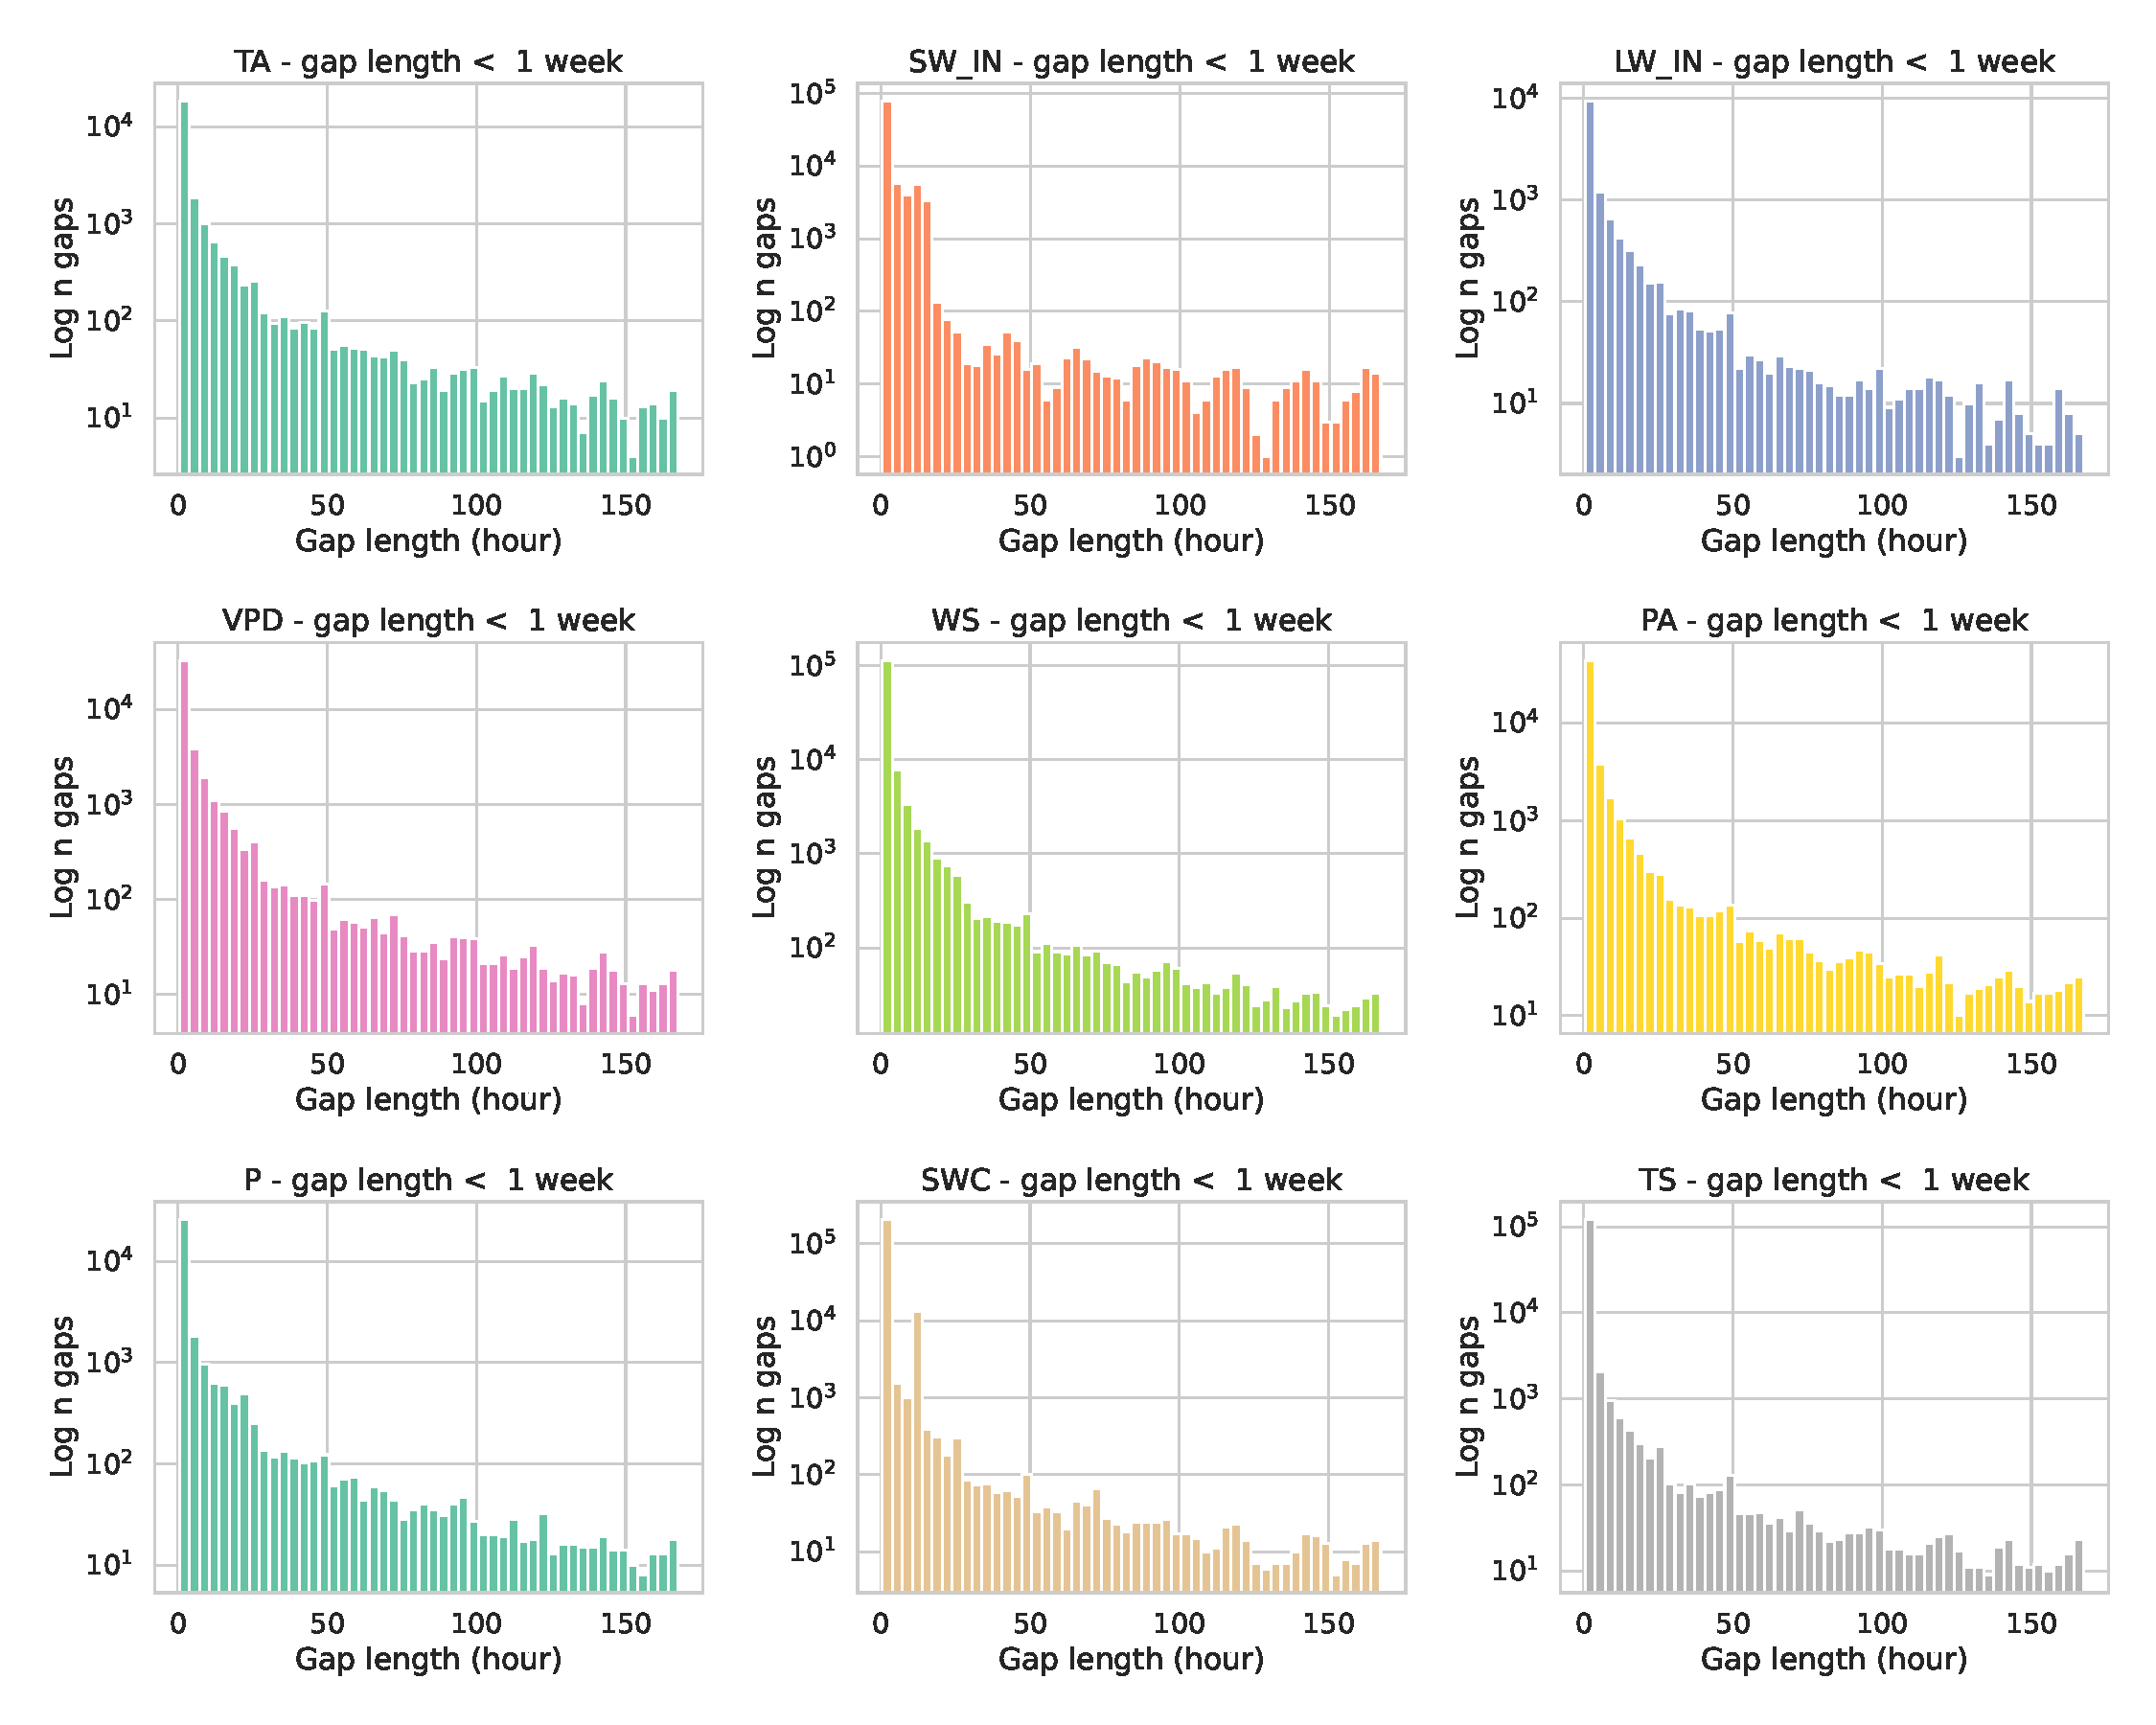
\includegraphics[width=\imgwidth]{gap_len_dist_small}}
\caption{Distribution of the gap lengths for gaps shorter than a week, for all sites in the FLUXNET 2015 dataset for meteorological variables. The y axis displays the logarithm of the number of gaps. The length of the gap is the number of records where the QC flag is different than 0.}
\label{fig:gap_len_dist_small}
\end{figure}

\section{Derivations}

\setcounter{equation}{0}

\begin{equation}\label{eq:deriv_predictions}
\begin{split}
    p(y_t^g \mid Y^{ng}) &= \int p(y^g_t \mid x_t) p(x_t \mid Y^{ng}) dx_t\\
    & = \int \norm{y_t^g}{MHx_t + Mb}{MRM^\top} \norm{x^s_t}{m^s_t}{P^s_t} dx_t\\
    & = \norm{y^{ng}_t}{MHm^s_t + Mb}{MRM^\top + MHP^s_tH^\top M^\top}
\end{split}
\end{equation}

\begin{equation}
\begin{split}
    MM^\top &= \begin{bmatrix} R^{1/2} & HP^- \\ 0 & (P^-)^{1/2} \end{bmatrix}\begin{bmatrix} R^{\top/2} & 0 \\ (P^-)^{\top/2}H^\top & (P^-)^{\top/2} \end{bmatrix}= \\
    &=\begin{bmatrix} R^{1/2}R^{\top/2} + H(P^-)^{1/2}(P^-)^{\top/2}H^\top & H(P^-)^{1/2}(P^-)^{\top/2} \\ (P^-)^{\top/2}(P^-)^{1/2}H^\top & (P^-)^{1/2}(P^-)^{\top/2} \end{bmatrix} = \\
    &=\begin{bmatrix}S & HP^- \\ (P^-)^\top H^\top & P^- \end{bmatrix} \\
    \\
    VV^\top & = \begin{bmatrix} S^{1/2} & 0 \\ \bar{K} & P^{1/2} \end{bmatrix}\begin{bmatrix} S^{\top/2} & \bar{K}^\top \\ 0 & P^{\top/2} \end{bmatrix} = \begin{bmatrix} S^{1/2}S^{\top/2} & S^{1/2}\bar{K}^\top \\ \bar{K}S^{\top/2} & \bar{K}\bar{K}^\top + P^{1/2}P^{\top/2} \end{bmatrix}\\
     & = \begin{bmatrix} S & S^{1/2}S^{\top/2}K^\top \\ KS^{1/2}S^{\top/2} & KS^{1/2}S^{\top/2}K^\top + P\end{bmatrix} \\
     & = \begin{bmatrix} S & HP^- \\ P^-H^\top & KHP + P\end{bmatrix}
\end{split}\label{eq:deriv_meas_update_sr}
\end{equation}

All blocks of $VV^\top$ are directly equal to $MM^\top$, but the bottom left one, which is equal due to the measurement update for the covariance (Equation \ref{eq:meas_update}).

% \paragraph{Standardized RMSE}

\begin{equation}\label{eq:deriv_stand_rmse}
\begin{aligned}
    \text{RMSE}_{\text{stand}} &= \sqrt{\frac{\sum_i^n (y^z_i - \hat{y}^z_i)^2}{n}}\\
    &= \sqrt{\frac{1}{n}\sum_i^n \left(\frac{y_i - \mu_Y}{\sigma_Y} - \frac{\hat{y}_i - \mu_Y}{\sigma_Y}\right)^2}\\
    &= \sqrt{\frac{1}{n}\sum_i^n \left(\frac{y_i  - \hat{y}_i}{\sigma_Y}\right)^2}\\
    &= \frac{1}{\sigma_Y}\sqrt{\frac{\sum_i^n (y_i  - \hat{y}_i)^2}{n}}\\
    &= \frac{\text{RMSE}}{\sigma_Y}
\end{aligned}
\end{equation}

\clearpage

According to the Examination Regulations, I hereby confirm, that I have written the present thesis independently and without making use of any other sources and
 tools than those that are indicated. I assure that the written version of this thesis corresponds to the digital version.

\end{document}

